\documentclass[11pt]{report}
%\usepackage{latex8}
\usepackage{times}
\usepackage{graphicx,ifthen,subfigure}
\usepackage{makeidx}
\usepackage{nomencl}

\usepackage{setspace}
\usepackage[colorlinks,linkcolor=blue,plainpages=false,pdfpagelabels=true]{hyperref}
\renewcommand{\nomname}{Glossary}
\renewcommand{\nomlabel}[1]{{\bf #1}\hfill}
\makeatletter
\renewcommand{\nom@verb}{~\newline\expandafter\strip@prefix\meaning}
\makeatother

\makeindex
\makeglossary
%\pagestyle{empty}

\newcommand{\ignore}[1]{}

%\renewcommand{\topfraction}{1.0}
%\renewcommand{\bottomfraction}{1.0}
%\renewcommand{\textfraction}{0}
%\renewcommand{\floatpagefraction}{1}

\newif\ifremark
\long\def\remark#1{
\ifremark%
        \bigskip
        \begingroup%
        \dimen0=\columnwidth
        \advance\dimen0 by -1in%
        \setbox0=\hbox{\parbox[b]{\dimen0}{\protect #1}}
        \dimen1=\ht0\advance\dimen1 by 2pt%
        \dimen2=\dp0\advance\dimen2 by 2pt%
        \vskip 0.50pt%
        \hbox to \columnwidth{%
                \vrule height\dimen1 width 3pt depth\dimen2%
                \hss\copy0\hss%
                \vrule height\dimen1 width 3pt depth\dimen2%
        }%
        \endgroup%
\fi}

%%\remarktrue
\remarkfalse

\graphicspath{{figs/}{curves/}}

\newcommand{\BL}{{\sf BL}}
\newcommand{\MR}{{\sf MR}}
\newcommand{\PR}{{\sf PR}}
\newcommand{\PIOB}{{\sf PIOB}}

\newcommand{\EG}{{\it e.g.}}
\newcommand{\IE}{{\it i.e.}}

\newcommand{\READPRIV}{{\tt READ\_PRIV}}
\newcommand{\READSHAR}{{\tt READ\_SHAR\_OR\_PRIV}}

\newcommand{\RECALLPRIV}{{\tt RECALL\_PRIV}}
\newcommand{\RECALLSHAR}{{\tt RECALL\_SHAR\_OR\_PRIV}}
\newcommand{\RECALLPRIVORIG}{{\tt RECALL\_PRIV\_ORIG}}
\newcommand{\RECALLSHARORIG}{{\tt RECALL\_SHAR\_OR\_PRIV\_ORIG}}
\newcommand{\RECALLINV}{{\tt RECALL\_INV}}

\newcommand{\RESPINV}{{\tt RESP\_INV}}
\newcommand{\RESPCANCEL}{{\tt RESP\_CANCEL}}
\newcommand{\RESPDATA}{{\tt RESP\_DATA}}
\newcommand{\RESPSHAR}{{\tt RESP\_SHAR}}

\newcommand{\DATASHAR}{{\tt DATA\_SHAR}}
\newcommand{\DATAPRIV}{{\tt DATA\_PRIV}}

\newcommand{\WRITEBACK}{{\tt WRITE\_BACK}}
\newcommand{\UPDATETAG}{{\tt UPDATE\_TAG}}
\newcommand{\UPDATEDATA}{{\tt UPDATE\_DATA}}
\newcommand{\ALLOCPRIV}{{\tt ALLOC\_PRIV}}

\newcommand{\LDBIAS}{{\tt ld.bias}}
\newcommand{\LD}{{\tt ld}}
\newcommand{\LDC}{{\tt ld.c}}
\newcommand{\LDA}{{\tt ld.a}}
\newcommand{\LDS}{{\tt ld.s}}
\newcommand{\LDACQ}{{\tt ld.acq}}
\newcommand{\PREFEXCL}{{\tt lfetch.excl}}

\textheight 9in
\columnsep 1.0pc
\textwidth 6.5in
%\headheight 0.0in
%\headsep 0.0in
\oddsidemargin 0in
%\footheight 0.0in
\topmargin -.5in
\setstretch{1.18181818181818}

\begin{document}
\title{Vega Strike: Upon the Coldest Sea \\ Game Design Document}

\author{Ed. JS}

\renewcommand{\thepage}{\roman{page}}
\maketitle
\renewcommand{\thepage}{\arabic{page}}
\thispagestyle{empty}
\centerline{\bf {\Huge Acknowledgements:}}
~\newline
The structure of this document is inspired by suggestions from a Baldwin Consulting document on Game Design Documents~\cite{BaldwinGDD}.

\clearpage
\thispagestyle{empty}
\centerline{\bf {\Huge Revision History:}}
~\newline
\begin{itemize}
\item {\bf 0.0.1} \\
Initial skeleton.
\end{itemize}

\clearpage
\setcounter{tocdepth}{2}
\clearpage
\phantomsection
\addcontentsline{toc}{chapter}{\emph{Table of Contents}}
\tableofcontents
\listoftables
\addcontentsline{toc}{chapter}{\emph{List of Tables}}
\listoffigures
\addcontentsline{toc}{chapter}{\emph{List of Figures}}
%\chapter*{Preface}
%\addcontentsline{toc}{chapter}{Preface}
%Welcome, intrepid reader, to the Vega Strike Universe - or at least a
document containing a lot of text concerning it and its design.

When we first started developing the current back story for VS, the
existing premise could be reasonably summed up as follows: ``An alien
species called the Aera are aggressively invading human space, and
there's this other group called the Rlaan who don't like either of the
humans or the Aera, but probably dislike the Aera more than the
humans'' - which is to say, someone out there had played StarCraft and
liked it. In the years since then, we've added a bit more, as the
somewhat larger size of this document may indicate. While this
document may take a bit longer to digest than the above one-sentence
summary, we happen to think it's worth the extra reading.

\section*{About this document}
This document is best described as a sort of ``design doc'' for the Vega
Strike Universe (hereafter often ``VSU'' -- this document uses a lot
of initialisms - please consult the \ref{Glossary:Glossary} section for any of them
that aren't clear). It contains a number of different things: general
cosmology and physics for the VS universe, back story for the {\it
Upon the Coldest Sea} game setting, discussions of design
philosophies, and discussions of the game-play-relevant implementations thereof. In that
it splits its time among sections discussing the design philosophy
behind the design of the VSU, sections best viewed as discussions of
the resulting decisions, and swaths of expository data dumps detailing
particulars of the backing fiction, it is an uneven document. However,
in serving all of the audiences it intends to inform, it would seem
difficult to achieve full blown elegance.

This document aims to do the following:
\begin{itemize}
\item Provide a cosmology and highlight key rules for the VS universe
   so that some intuition as to what is and is not likely to be canon
   can develop. This includes delineating where we are taking
   liberties with physics and where we are holding firm to our grip on
   reality. Moreover, this delineation must be addressed twice - once
   for the purposes of creating and editing fiction, and again for the
   artistic representations, which may not always correspond exactly
   to the ostensible VS reality (e.g. the VS universe demands that we
   have substantial radiators on starships during the {\it Upon the
   Coldest Sea} time period, but the artistic direction may resolve,
   on many craft, to token/symbolic radiator surfaces in order to preserve
   aesthetic and other artistic freedoms). Within the bounds of what
   has been declared possible in VS, we must likewise be sure to
   indicate where optimism is assumed and where the VS universe makes
   more pessimistic assumptions about how much of the possible is
   actually achievable by given groups at particular points in time.
\item Provide both back story and future-history for large-scale
  events, so that those looking to create stories set in the Vega
  Strike universe have both a backdrop to frame their stories in, and
  a set of future events to preemptively constrain continuity.
\item Codify game-play philosophies and examine the effect that universe decisions will have on potential game-play options, and vice versa.
\item Provide sufficient detail on relevant species, factions, and
  technologies, as they appear in the UtCS setting, that artists can
  become familiar with the subjects they are to portray.
\end{itemize}

Before going any further, an important point - at the time of this
writing, this document is far from finished. It is not polished, it is
not, in some places, even fully skeletal. This document will change
over time. The odds approach certainty that some pieces of it will
eventually require retconning and that others will be missed during various
evolutionary changes and thus become
desynchronized. Still, what is in this document, even in its
unfinished and mercurial state, is the VS canon until changed, and
should not be ignored, skipped over, or otherwise elided lightly.

\section*{Who is this document for?}
It should be acknowledged that this is a somewhat oddly targeted
document in there are several audiences that it needs to inform. These
audiences are rather diverse, ranging from texturing artists to
writers working on player-driven plot-lines. In keeping with this
mixed-usage model, a fair portion of the people who read this document
will not need to read the entire document. Artists, for example, are
encouraged to read the overviews in Chapter~\ref{chapt:overview}
before jumping to the portfolios portion of this document
(Chapter~\ref{chapt:portfolios}), but may find little use for much of
Chapter~\ref{chapt:timelines}'s treatment of VSU time-lines. That said,
those looking to do any additional fleshing out of the framework are
strongly-advised to read the whole document with some degree of
attention before considering pushing forward with such an undertaking.

\section*{Additional notes on reading this document}
Certain sections of this document may contain passages in the first
person. These can be assumed to be written by {\it JS} unless
otherwise specified or indicated by context. 

Sections not otherwise
specified should be assumed to be written from an omniscient
viewpoint. In particular, some of the Appendices, such as Appendix~\ref{appendix:Species} and Appendix~\ref{appendix:Factions} are {\bf NOT}
written from an omniscient viewpoint, and are intended to represent
generally available knowledge that would be easily obtained in the
UtCS time period. For information intended to player-visible, please
pay special attention to said appendices, {\it especially} when they
are in conflict with data from the omniscient viewpoint sections of
this text, as the difference is likely an intentional implementation
of ignorance or misconception on the part of the VSU's inhabitants.

Some parts may be so unpolished or incomplete as to be difficult to
parse or otherwise comprehend. Similarly, they may use non-standard
vocabulary or jargon that has yet to make it into the glossary or rely
on mention of external sources that have not yet been appropriately
added to the references section. However, these shortcomings are not
cause for ignoring the sections in question, but rather are cause for
developing questions pertaining to said sections, thereby prompting
their improvement. For insight, consider this previous VS-related
example of communication breakdown, one is told that ``X sounds like a
campanile'' and comes back with a sound for X that has no relation to
bell towers with an explanation along the lines of ``well, I didn't
know what a campanile was, so I just did something nice.'' The root
cause (campanile is apparently an insufficiently common word and
should be defined) is left untreated, the work in question balks
canonicity, and some fair bit of time may well have been spent on
something that could have been rectified with a simple clarifying
question. While asking the reader to invest additional energy in
comprehending the more tenuous portions of the text and actively
responding to their shortcomings is a more than normal demand,
attempting to use an incomplete document as a guide is a somewhat
awkward undertaking, and comes with its additional burdens. Those not
interested in walking through the textual debris and construction
zones are welcome to wait - we do eventually plan to make this
document fit for normal reading - but the realities of the schedules
we're working on means that this document will continue to see use in
various stages of its genesis, refinement, and extension.


% LocalWords:  UtCS Aera Rlaan StarCraft VSU initialisms retconning retconned
% LocalWords:  JS VSU's


\chapter{Game Overview}
\label{chapt:overview}
This chapter provides an overview of some of the high-level aspects of
the Vega Strike Universe and the design philosophies at play. It
indicates with broad strokes what forms of content and approaches to
topic matter will be appropriate for the Vega Strike Universe. Section
~\ref{sec:thingsseeninVSU} introduces a number of things which one
should expect to see in any finalized (though not necessarily interim)
depiction of the VSU, while Section~\ref{sec:thingsnotinVSU} notes
categories explicitly {\bf not} suitable for being present in the VS
universe. Section~\ref{sec:VSphysics} outlines the key assumptions of
VSU physics, notes divergences from likely physical realities, and
briefly delves into some of the ways in which VSU physics will
manifest in gameplay. Section~\ref{sec:plottingphilosophy} discusses
our position on the role of the player with respect to the progress of
galactic events, and the resultant bifurcation of plot into the
galactic-scale plot (as per the timelines in
Chapter~\ref{chapt:timelines}) and the personal plot segments that
will directly involve the player character. Section~\ref{sec:VSthemes}
introduces common themes that will be appearing in the VS Universe and
galactic-scale time/plot-lines, and may likewise be echoed by the
smaller player-scale plots. Section~\ref{sec:groupintuitions}
concludes the overview chapter with some advice geared toward
internalizing intuitions for various human and alien groups present in
the VSU during the UtCS period.

\section{Things that should (eventually) be seen in the VS universe}
\label{sec:thingsseeninVSU}
\begin{itemize}
\item FIXME
\end{itemize}

\section{Things that should not / will not be seen in the VS universe}
\label{sec:thingsnotinVSU}
\begin{itemize}

\item Interventionist deities or agents thereof

Whether or not a divine being or beings exist in the VS universe is
irrelevant. Neither evidence nor action by any such entities occur in
the VS universe.

\item Interventionist deities or agents thereof (pretending to be aliens)

The term ``god-like'' could easily be applied to any type II or type
III civilizations (Kardashev scale~\cite{Kardashev}), or even members
thereof. This does not make them actual gods. Nor should they be used
as stand-ins for traditional human deity-figures, redemption figures,
moral archetypes and so forth. That they are profoundly powerful does
not make them well intentioned, infallible, or even necessarily
wise. That they are ``god-like'' in power merely denotes them as
powerful enough that they possess a potential for actions at greater
scales. It is worth noting, if nothing else, the number of powers
previously reserved for gods that even our own civilization (not yet
even a type I civilization) has already secured for itself without attaining
any shred of divinity.

\item Absolute Morality, embodiments thereof, and anthro-exclusive destiny

There is nothing intrinsically {\em good} or {\em evil} in the VS
universe, be it an action or an entity. More importantly, there is no
external guidance toward ``the good'' or away from ``the evil'' that
acts as some imperative societal force, nor a presumption that what we
consider elements of ``the good'' will prove to yield higher
survivability than aspects our modern societies do not deign to
associate with goodness. While it is certainly more difficult to see
some actions as beneficial than others, as there is no presumption of
an external calibrating entity in the VS universe, such judgments are
societal, and their merit only capable of being judged properly long
after any associated actions have been taken. Additionally, the
continued existence of humanity should not be blithely assumed to be a
universal ``good''. While humanity and their descendants will play an
important role for a certain time-period in the VS universe, this is
happenstance, and not providence. Indeed, much of what happens after
UTCS is in many ways a decline of humanity and the supplanting of
humanity by its children.

\item Magic (as magic)

The following, among other things not listed, do not exist (at least
as people currently describe them) in the VS universe: ESP, psionics,
talking to the dead, spiritual possession, auras, telepathy,
telekinesis, purity of essence, and clairvoyance. Events in the VS
universe will not be determined, nor even affected, by `fate', gods,
prophecy, or other elements of the supernatural.

\item Magic (pretending to be technology)

While Clarke's law posits that any technology, sufficiently advanced,
is indistinguishable from magic, the converse is decidedly {\bf not}
true in the VS universe. Just because we can think of some magical
means for doing something does not mean that any technological
implement, no matter how advanced, can ever achieve the same
effect. This is not to be confused with things such as fusion reactors
which we have firm understandings for how, in general principle, one
might work, but cannot fathom how to build a practical one. Allowing
leeway for overcoming implementation difficulties, or even profound
knowledge gaps is a different beast altogether than positing something
to exist which we can already know to be in violation of numerous
aspects of our model of reality. This means no perpetual motion
machines, no instantaneous galactic communication (although we do
still regrettably violate causality with non-instantaneous FTL), no
living-super-armor (it's just a fad fuelled by, one presumes, a poor
understanding of high-tech carbon composite materials and the sorts of
metabolisms needed to produce such on the fly.), no life-force, no
ascension, and no ``energy-beings'' without a concrete definition of
the sorts of energies involved (i.e. ``being existing as patterns in
EM waves'' is OK, but ``ascending to pure energy'' is just pandering
to a magical reality, all apologies to Stargate, Babylon 5, etc.). We
must strive to differentiate the unlikely (even perhaps sometimes
coming close to the borders of implausibility), which is fertile
ground for science fiction (e.g. room-temperature superconductors)
from the truly magical masquerading in the guise of science
(e.g. though I do enjoy the series, most Doctor Who episodes are
fantasy, not science fiction) and from fundamentally unsound
propositions passing themselves off as profound knowledge or advanced
technology (e.g. splitting the beer atom, gaining mutant powers from
gamma radiation, almost anything from the movie {\em What the \#\$*! Do
We (K)now!?}, entities that gain mass without consuming anything,
re-spinning the earth's core with a hydrogen bomb, neutrino weapons,
hacking alien mother ships with a laptop, instantaneous evolutionary
accelerators, ``polarity reversal'' as the answer to everything, and
claims that ``humans only use 3 percent of their brains'').

While the VS universe allows some liberties with known or
expected physics for the sake of plot and game-play possibilities, we
are bound by the laws of physics unless explicitly relieved from said
limitations. Deviations from our base physical reality have a nasty
habit of causing cascading implications that aren't desirable, and
should only be undertaken with both good cause and firm caution. 

We make explicit and limited exceptions for FTL, shields, and other
related space-warping technologies which we bin under
``gravitics''. Gravitics is known to be junk-science, but, as magical
additions to reality go, can be presented in a reasonably
self-contained fashion as long as nobody stares too long and hard at
it. FTL is, for better or worse, necessary, and shields are, if not
necessary, sufficiently desirable and expected that we've made room
for them.

Toward the end of limiting the sickly spread of junk science and
outright silliness into every aspect of VS, we should avoid
technobabble like the plague that it is. While it's fine, in documents
such as this, to ponder to some degree how some of the VS tech is
presumed to work in order that we can coherently and consistently
describe the properties of objects using said tech, the user should be
heavily insulated from such discussions. Firstly, what the user needs
to know are the end effects (e.g. does it pierce shields, how does the
range fall off, how much energy per second does this reactor provide,
etc.) and what the useful inferences they can make are (e.g. this is
a ``shield-type'' weapon, other ``shield-type'' weapons will have
similar properties) more so than any nitty-gritty made-up details of
how tech we don't actually know how to build works. Secondly, if we
attempt to explain how something no one knows how to build works,
we're almost certainly going to come off sounding like either outright
fools (for using real terminology incorrectly) or as purveyors of
gobbledygook (for using unreal terms randomly). Star Trek is the
perfect example of what {\bf NOT} to emulate here. There will be no
``transferring of power from the rear neutrino phase shift emitters
to synchronize our tachyon-positron field into a stable
co-phase matrix''. In the long term, it will only be held against us.

\end{itemize}

\section{Physics and Technology in the VS Universe}
\label{sec:VSphysics}
\subsection{On Weaponry, Defense, and Damage in the VS universe}

So, assuming one has the ability to diddle with the surrounding space
(leaving discussion of whether this, or any other stated principle,
was/could be a good choice for a fundamental assumption to another
time) how might one construct a shield?  Well, I thought perhaps one
could set up something based around gravitic shear forces (locally
violent, but, with opposing forces mostly canceling each other out at
greater distance due to super-linear falloff).

I then figured it would probably be worthwhile to augment such a setup
with an EM component, so as to assist against charged particles, as
charged particles are easy to accelerate, and therefore a likely
choice in assorted weapons systems. So, when descriptions (minimal as
they were) were written for shields, they were referred to as
providing a combination of gravitic and electro-magnetic protection.

Now, where did this lead me (at least as far as I saw it) - almost
everything except for something that looks like a shield should
penetrate a shield in some manner to some degree.

(a brief aside: ship collisions are somewhat outside the scope of this
post - suffice it to say that they should be much more catastrophic
than they are, but the reason is not related to shields - it's that
our damage model only works on energy right now, and doesn't look at
time related components, so if a ship smacks into something at 300m/s
and bounces off at 100m/s in the opposite direction we apply damage
due to the loss of kinetic energy, but don't currently address the
problem that, if this collision took 1/10 of a second, the ship
experienced an acceleration of 400g's, the pilot should be paste (even
assuming some (limited) means of inertial compensation as a cheap way
to warp space may be deemed to provide), and the ship should be
assorted bits of fine debris - this is a bug, a feature failure in
need of fixing. We don't have a model for acceleration tolerance,
clearly, we need one.)

Shield effects, by category:
\begin{itemize}
\item LASERS and other coherent EM radiation 

hard to get a beam of light to interact strongly with this setup at
all (unless one assumes that photons passing through the distorted
topology can be convinced to dump energy and shift down the frequency
spectrum in return for degrading the desired topology - but the more
that I've thought about that, the less it appeals to me, so let's not
spend much time there) but it might interact weakly, de-focusing the
beam. For low frequency radiation, de-focusing is going to be quite
detrimental (in terms of the likelihood of armor being capable of
dealing with incoming beam) but one imagines that xasers and grasers
are still going to be quite damaging even if the incoming beam is
distorted and defocused. Hence, at best, fair protection against low
end laser weapons, to negligible protection against high-end laser
weapons. This translucency (not transparency) has the benefit of making
it easier to explain how EM spectrum sensor data gets in, but causes
some problems with pilot-line-of-sight (upon further reflection, I've
come to the opinion that chuck raised an excellent point with respect
to his comment about the insistence of early astronauts on capsule
windows - there are only two major human groups in the VS universe
with pilots that likely wouldn't demand the same, if not windows per
se, then some semi-direct optical access (I also briefly, and not in
particular seriousness, pondered the notion of an "optical fuse" )-
but this delves into a whole other train of thought, so I'll stop it
here for now.)

\item Solid objects

should interact fairly strongly with the shear forces. Complex objects
could end up giving up non-negligible amounts of energy in undergoing
deformation or otherwise smacking into bits of themselves. However,
given high initial velocity, sizable portions of the incoming
remnants of the object will not be sufficiently diverted and will
still intercept the target. This is still a preferable scenario, as a
defocused impact of something more resembling dust and shrapnel should
be a lot easier for armor to handle than an intact shell. (Unless of
course, one doesn't have armor, in which case one may have just traded
one set of holes for many sets of holes.)

\item Particle beams

A) Charged - high velocity makes them hard to divert with the
gravitics, again just gaining a defocusing, but that's what the EM
systems are there for helping out with. Still, in the end it's just a
very good defocusing and diverting, and can't be expected to stop all
the incoming particles completely.

B) Neutralized - EM field doesn't help in any meaningful way,
defocused, more-so than a laser, but protection is pretty poor, and
it's mostly up to the armor.

\item Plasma 

A)Net-neutral, or B) net-charged clouds of high temperature ionized
particles that are likely to be fairly effectively diverted by an EM
field unless the plasma density was quite high at the time of
interaction (still efficiently diverted in such a case, but perhaps
not effectively).

\item Shields and shield-like weapons

Directly act upon the topology created by the shields, significantly
degrading them. However the directness of their interaction also means
that their effects do not penetrate the shields.

How I saw this playing out in terms of game mechanics: 

Firstly, as shields degraded (topology becoming unstructured, shear
forces going away), anything that penetrates a shield already would
penetrate more. The EM field wouldn't degrade in the same manner as
the space-warping component, but it was only useful in mitigating
charged particles anyway.

\end{itemize}

Weapons, by category:
\begin{itemize}
\item Lasers

would seem to be quite nasty beasts in that they mostly ignore
shields, especially at higher frequencies, except that lasers have
lousy energy efficiency, especially at higher frequencies, and
especially given that laser inefficiency tends to materialize as waste
heat. Thus I saw lasers as weapons with extreme cooling problems,
either resorting to open cycle cooling (venting coolant = limited
ammo, limited re-fire rate) or {\em very} slow re-fire rates (also a source
of perhaps interesting complexity if/when any form of heat modeling
gets implemented). Likewise, the higher frequency lasers would be
prohibitively expensive and potentially bulky beasts, probably not
found in small craft. Additionally, as they don't interact strongly
with shields, they wouldn't be good weapons for degrading them
rapidly. Range would be good though,

(lasers don't degrade as the inverse square, but diffract according to something along the lines of 

RT = 0.61 * D * L / RL 
where: 
RT = beam radius at target (m) 
D = distance from laser emitter to target (m) 
L = wavelength of laser beam (m) 
RL = radius of laser lens or reflector (m) 
) 

\item Solid objects 

Lower energy requirements (could also have internal energy sources, as
per rockets), easier cooling solutions, good rates of fire, degraded
by shields but degrade shields, and become increasingly effective as
the shield degrades. Limited ammunition. Can be augmented (at
increased size/cost) by addition of shielding, and/or nuclear or
anti-matter warheads. At the (expected relative) velocity these would
be impacting at, conventional explosives would not be useful
additions. Damage does not decrease with range (although for reasons
of limited processing power, a "max range" still needs to be specified
engine level).

\item Particle beams

A)Charged - low yield electron beams can already be made with very
high efficiency - but cranking up the power will drop the efficiency a
lot. More importantly, any charged particle beam suffers from severe
thermal and electro-static bloom. The constant on the super-linear (I
believe it's actually an inverse-square) decay in beam density can be
helped by using more massive particles, or accelerating to
relativistic velocities for the sake of time dilation, but at the
expense of efficiency (significant relativistic velocities are a
{\em huge} energy investment, neutrons are dead weight to an EM
accelerator, and only so many electrons can be conveniently added to
or removed from an atom). To make matters worse, one's ship will
accumulate net charge if repeatedly firing a charged beam, unless the
excess charge is bled off somehow (I've seen indications that
alternating between positive and negatively charged firings is a "bad
idea (tm)" due to creating a current loop involving the vessel). So,
to sum up, the range is pretty bad, the efficiency is questionable,
there's probably a hell of a re-fire delay as one cleans up the charge
accumulation problem, and EM fields can do a lot to defocus the
incoming beam. However, if you are close enough, and your particle
density is high enough, then what does get through would do nasty
things to armor, surface mounted electronics, and throw off lots of
secondary radiation.  

B) Neutralized - (and by neutralized I don't mean "neutron beams",
because I haven't the foggiest idea how to generate or accelerate them
effectively in anything resembling a coherent beam unless we start
talking about space-warping that is probably powerful enough that'd
we'd have to go back and revisit the whole "can't do to much to
photons" issue which I'd rather not, and besides, that would probably
mean that shields were impervious to just about anything... which is
rather much not the goal either) more specifically, a beam of
particles that has been rendered charge neutral; one in which
oppositely charged particles (likely electrons) are added back in
after acceleration (both must have been accelerated) to neutralize the
beam. This will almost certainly defocus the beam, and again almost
certainly drop efficiency even lower. However, it avoids the local
charge accumulation problem, this removes electrostatic bloom, leaving
only thermal bloom, increasing range, and it also negates the
effectiveness of EM fields to disperse the beam at the
target. However, it also negates the current and charge accumulation
effects on the target that might damage electronics. Still, plenty
unpleasant on impact, only mildly affected by shields, but range isn't
as good compared to lasers, and efficiency is only questionably
better, and could easily raise similar cooling/re-fire issues.

So, as for beams - mediocre range due to bloom effects, efficiency
questionable, neutralized beams achieve good penetration against
shields at cost of even lower efficiency, charged beams have lousy
penetration against shields, but can probably be used in efforts to
disable the target's electronics (at the least, those present on the
surface, or accessible by necessity (engine/reactor) - the core
protected elements are going to have to be in some Faraday cages with
optical links to the externals (optical links don't like shear forces
though, so they could break with some probability upon impact or
impact resembling damage). Ammunition (the particles in question)
necessary, but in sufficiently small quantities per firing that it can
either be ignored or modeled as extremely cheap, small, and
plentiful. Some noticeable degradation of shields due to some
interaction.


\item Plasma 

Last I investigated, unless there's some way to make plasma somehow
generate its own magnetic fields of exceptionally interesting (read:
somewhat absurd) strength, or one wants to accelerate the plasma to
very high velocity (which would start to look something more like a
shorter pulsed version of the the beams above), it's not going to be
an effective weapon at anything beyond the shortest of ranges, because
it expands like no one's business (our dear friend the inverse square
law, but with indications of unforgiving constants, the prevalence of
plasma weapons in many sci-fi works notwithstanding) and in every
direction. High-tech flamethrowers with interesting electrical
properties are cool, but not very effective unless one is close enough
to read the serial numbers on the target's fuzzy dice, never minding
the effects of EM fields on ions, which further limits effectiveness.

In short, one could build the bolt (short pulse) rather than beam
version of a particle beam, and it would be rather similar to the
particle beams, and not what one traditionally calls a plasma
weapon. Or, one could build a reasonably efficient plasma weapon, but
be limited by rapid falloff to the shortest of ranges. Ammo for plasma
weapons should be in the dirt cheap, small, and exceptionally
plentiful category. If you're actually close enough to get any
reasonable number of particles past the EM fields, you'll do nasty
things to the electronics, and you can probably afford to keep firing
for a while. Shield degradation can be somewhat more pronounced than
particle beams if more matter is being thrown at the target.

\item Shields-and shield based weapons

Ammo, none. Shield penetration, none. Efficiency, mediocre-poor, hence
re-fire, fair-slow. Target shield degradation better than any other
damage source. Transmitted damage after shield collapse (topology
unstructured) worse than any other damage source, but non-zero. Damage
vs. unshielded objects significant.

\item Missiles

Mostly depends on warhead type. Shielded kinetic is one option, single
shot weapons of various types also options, as are bomb pumped lasers
or simple nukes. Ultra-low-yield (0.5 - 1 ton range) fusion warheads
are presumed commonly available (preferable to chemical explosives due
to the manner of transmission of the energy, namely, high frequency
radiation and neutrons).
\end{itemize}

\section{Philosophy of scope and goals for plot and protagonist}
\label{sec:plottingphilosophy}
There are a number of classical archetypes for heroes and their
journeys. One can wander down the Freudian/Jungian pages of Campbell's
{\em Hero with a 1000 Faces} and see everyone from Siddhartha to Luke
Skywalker.  That's not the sort of hero we're looking for because that
isn't the sort of story we're looking to tell. I'm not interested in
crafting a thinly disguised morality play. I'd prefer to limit the
degree to which things devolve into an expression of teenage fantasies
of godlike empowerment - Dragonball Z is NOT what I would consider a
good starting point for much of anything, even ignoring the sequel
strangling power growth whereby planets are being absentmindedly
smashed. Likewise, the standard Square RPG wherein the young weakling
levels up repeatedly until he becomes a veritable force of nature that
the course of all history depends upon is NOT a desirable goal. Even
the more subdued Freelancer variant thereof is something to be avoided
- especially the standard "enemies keep getting more powerful just to
match the player's progress despite the fact that this means that
later stage enemies could slaughter entire civilizations from earlier
in the game" and "fate of humanity rests upon the player"
problems. Privateer levels of player significance are probably as far
as we should consider treading, and, where possible for VS, I'd like
to move the bulk of the significance to before the player takes
control of the character. I find it preferable to have a character
intrinsically with some significance and then let the player do with
that what they will rather than to force a player down a path that
will cause them to become significant - I think it's much more
interesting to have, as a purely hypothetical and unrelated-to-VS
example, a scenario where a powerful entity decides to spend its time
surfing, gambling and sowing its wild oats instead of saving the human
race because it just didn't feel the motivation or didn't want to risk
it than to yank the player incongruously along every time they start
to wander down a path that doesn't take them toward becoming some
"powerful entity". Cosmic significance for an individual is really
difficult to not screw up in SF, less so perhaps in fantasy where
there are easier outlets for suspension of disbelief compatible with
the base universe. Even if the rest of this paragraph falls out of
your heads from my rambling text, here's the point I want to make
clearest - cosmic significance is not necessary for compelling drama
or even more generally, good stories, drama or otherwise. In Catch-22,
Yossarian never strikes a deathblow against the Nazis. In All Quiet on
the Western Front the protagonist accomplishes little except surviving
only to die, and if that's not a compelling story for being too far
from the SF vein then ponder Blade Runner - the world is just as
screwed up in the end as in the beginning, but one is consumed by the
story of even the few people (and replicants - not all interesting
characters need be truly human) involved. In a more recent pop
setting, Law and Order doesn't feature gods and monsters, but has
audiences so hooked they keep spinning off companion series. Even
looking at the new Battlestar Galactica series (the first season, at
least ;-) )shows the strength that can come from focusing on human
interactions and frailties even in a dire and cosmically important
situation. In short, it is sufficient for the story the protagonist is
directly entangled in to be important to the protagonist and those
around him/her.

This is not to say that we should avoid big stories, epic stories of
sweeping scope. Merely, there appears to be frequent confusion that,
in order to tell the tale of Moby Dick the player somehow must have to
be either Ahab or the Whale! This is why, for the purposes of story
development for VS, I want to distinguish between the big plot and the
little plots. The big plot is an epic canvas, a great, boldly painted
backdrop with thick lines and firm colors against which and within
which smaller events are set, contrasted, and constrained. The big
plot should concern itself with what would be written in history texts
after its conclusion, whereas the little plot should concern itself
with what its surviving characters would tell their grandchildren
about what they were doing during some chapter in the aforementioned
history text. The epic actions should remain mostly constrained to
actions of sufficiently sized groups, those who command such groups,
intelligible chance happening, and other such mechanisms as are
required to create the epic sweep of time and space beyond the ken of
small beings. This is not to say that players in the little plots
cannot affect the events of the big plot, it is rather they need not
do so, and are likely to only have extraordinary effect when they have
performed extraordinary action. The converse, of course, is not true -
actions that occur in the big plot can clearly have profound and
immediate or delayed and subtle effects upon the player - the fall of
a government will obviously change a player's experience if they were
to go visit that region, and the stresses of a war economy should
become apparent in various pricings, patrol levels, availability of
side tasks, etc. To rein things back a bit from the general to the
specific, UTCS will, at root, be the story of one man's life during
wartime, seen through his eyes,

As for characters themselves, let the fools be fools and the sages,
sages. However, no matter how cynical one may be, constructing plots
that require the vast majority of entities involved to be either
blithering idiots, willfully ignorant, or (even worse)
schizophrenically swinging between brilliance and incompetence, is
poor craftsmanship - although there is something to be said for
wandering down a cliche path and then twisting it at the end to inform
the audience that you were aware of the cliches - Alan Moore's Watchmen
has some great examples of such twists. Hinging a plot on some
important thing not being known isn't a bad thing, but hinging a plot
on an otherwise perfect plan crafted by keenly intelligent planners
having a "fatal flaw" that allows "good" to triumph over "evil" is
just plain old fashioned bad storytelling and magical thinking at
that. Let me be clear on this - there is nothing good or evil in VS,
but the thinking of some group therein terms it so (my apologies to
the Bard).  Good and Evil is good fodder for children, but, at the
risk of alienating the vast potential audience of the unnuanced, to
the degree possible and appropriate (stories in the Rimward of Eden
setting, for instance would be reasonable places for "coming of age"
themes, even if it's an Aera coming of age), VS should deal with the
more complicated, and frankly more interesting, problems of adults (to
be honest, everyone who's been a teenager already did the teen angst
thing -there's no reason to keep reveling in it, even if many of us
can't always keep from doing so). If we manage to get ourselves
accused of moral ambiguity, of an uncomfortable gap between actions
noble and actions necessary, we're probably on the right track
(consider, for instance, the Andolians - their work with the AI Quorum
in creating the Grandchildren will help ensure the continued existence
(and local importance) of humanity, but they're also responsible for
billions of cold, calculated human deaths during the Fraternal war,
etc.).

The VS universe has strong existentialist influences - such is (my)
life and art does tend to imitate life J. However, that is not to say
that the goal is for VS to become an emo angst-fest of ennui. At the
beginning of UTCS, Deucalion is a bit of an emotional mess, but this
is to be expected. He's just gone through a traumatic event that
nearly killed him and did kill his best friend and (for
simplification) brother-in-law. He's rather a bit shaken, his life
plans have just been rudely interrupted, and, to add insult to injury,
the Aera have just started invading Forsaken space while Deucalion was
recovering from his injuries. It's a situation that is hobbled with
guilt and the impotence of any individual against the uncaring and
unnoticing motions of the universe. It's a situation ripe for
catharsis and, just as importantly, for life altering change - it is
therefore a good starting point for a player to take over a character
who already has a defined past. They can take the character in rather
different directions without it breaking all suspension of disbelief,
as "he cracked" and "you're not the same since XXX" are easily
intelligible human reactions to tragedy. At the same time, they can
use the existing past and the benefits and limitations it has bestowed
upon the character as either guide or leverage - his past gives him
skills that make him useful, hence a target for interaction with other
entities, and it limits his direct involvement with governance or
military forces. As he's already left the Protectorate navy, he can
much more believably stray further, or wander back - the choice is
his, and thus, the choice is the player's.

There is always the issue in an open-ended game of when things end -
where is the resolution? For UTCS, the big plot will advance whether
or not the player does too much. If one only wants to see what happens
in the big picture, one need only play a bit, and then play a
(safety-seeking) waiting game - in doing so, one has played out a
rather boring life, but it's a player's choice, and, if they aren't
actively playing, then they won't get to see the effects.  For UTCS, I
think having a number of soft-endings for a set of little plots
(hence, the plurality) is the best choice. Profession/lifestyle
specific plots can have an apex or plateau if not a conclusion. The
closest gameplay that comes to mind is the guild-leveling in
TES:Oblivion, but the pace of advancement in the Mage's guild seemed
less than proportionate to the tasks at hand, very gamish, but I
digress.

\section{Themes in Vega Strike}
\label{sec:VSthemes}
One recurring theme that is present in the overarching VS universe
story (although echoes of it will be seen in the player stories as
well) is that of intergenerational relations, of parents and their
children, in this case, the figurative species-children of various
groups and the effects that the actions of those who came before them
have on their own development. Our parents are our first gods, and
even if they succeed as parents, they will always fail us as gods. I
thought it would be particularly interesting then, to start the story
off with a parental group that really was, in many ways, godlike - but
still failed, and in their greatness, had their failure cast a
commensurately large continuing shadow over those who came after them.

VS, however, as much as the TWHON may impact the events that unfold,
should not be seen as a story about them. Their day, and indeed, their
greatness, and even their existence as anything but vague and warped
shadow of what they once were, has long passed. While it is worthwhile
to understand their place in the story, I would caution giving them
too lavish a portion of our attentions - gods may seem interesting,
but stories about people are much involving in the long term, if for
no other reason than we're not particularly good at portraying things
beyond ourselves in any closeup detail. It's easier to believe it's
not a man in a rubber suit if the behemoth is only seen at distance,
from the corner of the eye, or, as I would prefer it for most portions
of the VS timeline, evidenced primarily by what they have long since
wrought. This likewise removes many burdens of contemplating what
godlike beings would do interacting with the likes of us, or even our
post-human successors -- with the action in the past, we can leave
many motives mysterious, and focus on how characters more like
ourselves must deal with a reality of consequences, and not the
possibilities of dead gods.

\section{How to think about various groups}
\label{sec:groupintuitions}
This subsection isn't designed to give you all of the info on a given
group (check out one of the appendices for that). What this subsection
{\bf is} designed to do is to give an idea of what frame of mind one
should be in when considering a particular group in the VS universe
and how that group relates to others, themselves, and their
surroundings.

\subsection{Humanity}

One might think this part the least necessary group to consider, but
it's actually the most tricky. As humans, we've got a pretty good idea
of how humans operate. As we drift away from our current conceptions,
either confusion or disbelief can ensue. And we're going to have to
drift away a bit here, both for groups with trans-humanist directions
or aspirations, and simply because of the 1200 year gap between
ourselves and most of the VS cultures.

\begin{itemize}
\item {\bf Rule number one} - These are not the people around you. At least, many
of them aren't. The people of the 33rd century, by and large, bear
less resemblance to you than you do to a 10th century peasant - this
much is to be expected.

\item {\bf Rule number two} - Some of these "people" REALLY AREN'T the
people around you - at all. It's not just the cultural gap. Thinking
about the Purists as fairly normal, if scared, people, the Unadorned
as somewhat nutty religious people, the Forsaken (even more like
modern man than the Purists) as bitter people, the Highborn as
self-absorbed (and perhaps mildly self-deluding) people and the
Merchants as greedy people can lead to somewhat reasonable grips on
how these groups operate - they are, at heart, fundamentally still
human, if culturally distinct from today's climate. Even the
Mechanists can be superficially grokked by starting with a zealous
level of self-hatred directed at the limitations of their human
bodies. However, thinking about the Andolians or Shapers as just human
will delude you, and lead your conclusions astray. They are not yet
alien, but they are intensely foreign to the humanity we are familiar
with; they no longer think like us. The Andolians, collectively,
haven't forgotten anything meaningful for over 900 years. Each
generation grows up with immediate and nearly innate access to more
information than each generation before. They are connected, not just
in the simple physical sense of their link, but also in social senses
that modern man simply isn't. They don't think about self and the
other in the same way we do - they can't. The Shapers have adult minds
by the age of 7 and even their dullest healthy member surpasses most
modern humans. They are a society whose rate of idiocy, mental
defects, physical defects, malnutrition and insufficient pre-natal care
is so microscopic, their disease rate so low, that one it it suffices
to think of them as a post disease, post illness, post weakness
society. Theirs is a society of extreme individualists that runs
smoothly because they're all up on the game that's being played -
duping the Shaper electorate makes bribing the Supreme court look like
something a drooling infant could accomplish by accident. We share
more genes with the SuSims than with the Shapers. They are not gods or
demigods, or any such thing, but to think of them merely as human, is
to do them insufficient justice.

\item {\bf Rule number three} - The "Purist/Luddite" test: while you need
not agree with the eponymous groups, if you can't understand on a
permeating, gut level why these groups are so obsessed with bounding
what constitutes humanity and what it means to lead a human life, then
you don't yet understand the "humans" of the 33rd century that inhabit
the VS universe.
\end{itemize}
Key differentiable human groups include:
\begin{itemize}
\item Andolians

It would perhaps be inaccurate to say that the Andolians are actually
friendlier than the other major meme-groups. More accurate would be to
say that they are more tolerant, as much because they can afford to be
as because it aligns with their outlook. They are, however, often seen
as patronizing or even condescending in their tolerance of other
groups. This is still seen as preferable to the outright disgust,
hatred, or dismissal that can often be experienced between the
meme-groups. The Andolians often refer to each other with sibling
terminology, the Klk'k, even the non-linked, with diminutive sibling
references (bro-chan, sis-chan, etc.), non-Andolian humans in the
protectorate as "steps" or "steppers", the Purth as "little ones" (an
ironic touch, given that the Purth are extremely large), and
non-protectorate humans as "cousins". Such references, however, are
made only in casual discourse, and in generally unambiguous fashion,
with actual relations being made pointedly clear.

\item Forsaken
\item Highborn
\item LIHW
\item Luddites
\item Mechanists
\item Merchants
\item Purists
\item Shapers
\item Unadorned
\end{itemize}

\subsection{The Klk'k}

They're wisenheimers, to a degree. Their sense of humor permeates
their civilization more so than ours, making for odd juxtapositions,
such as it being entirely appropriate to be cracking jokes while
fighting, murdering, or engaging in serious policy decisions. The key
to thinking about the Klk'k is this - as much as they may seem to have
progressed along remarkably parallel lines, they're still aliens. As
SF author Gregory Benford once said, "the thing about aliens is,
they're alien." The Klk'k are enough like us, compared to all of the
other aliens, and they can work with us, that we keep wanting them to
be like us and expect them to be like us - but they aren't like us,
and it's always disconcerting when they prove it. One must imagine
asking a Klk'k why they have just done something, having them explain
in what appears to be a rational fashion, and still just being
dumbfounded as to why they did what they did - between differences in
axiomatic values and divergence in the nuances of the explanation it
just wasn't the same way of thinking about the situation, and thus
they arrived at a different outcome.

\subsection{The Aera}

The Aera got the short end of the stick - they drew the bad lot in the
running for "butt of cosmic joke" (perhaps they failed to
appropriately bribe the AUTHORS). Their planet was unpleasant, their
position in the jump network was supremely non-optimal, their timing
was poor and made even worse by the fact that they didn't know that
everyone else was going to run out of real estate soon enough
anyway. They aren't boogie-men, they aren't monsters, they aren't
ravenous alien invaders. They are an abused and shortchanged group
looking to survive in a universe that has repeatedly shown itself
uncaring to their existence. If the Klk'k disturb us when we are
reminded that they are unlike us, the Aera disturb us most when we are
forced to realize that we are not as different as we might like to
think, beneath bodies that each considers extremely ugly. Their
viewpoint tends to be colored by suspicions and certainties of
antagonism, but these are the result of a profoundly guarded outlook,
rather than the delusions of a human paranoid. Aerans are actually
quite distinct as individuals, but their fundamental pack and
abstracted pack loyalty structures allow them to operate cohesively in
groups in a manner that seems far more lockstep, frighteningly
authoritarian, and homogeneous to a human observer than it actually
is. The individual is celebrated post-facto. A life's accomplishments
cannot adequately be judged until that life is completed, from an
Aeran perspective. Don't think of the Aera as bad, as evil, or as
inherently inimical to the other races - this would be a miscarriage
of justice, and not even an oversimplification, but an
untruth. Rather, empathize with their miserable initial situation,
even if the only sane way for humanity to deal with them, alien and
resolute as they are, is to shoot back at them.

\subsection{The Rlaan}

The Rlaan are intensely alien. If the Klk'k are frustratingly alien,
and the Aera are at times painfully alien, then the Rlaan are
mind-bogglingly alien. They are, in fact, so alien that we can't
really understand how alien they are, because we can't identify what
in their behaviors is just complex and what is derived from more
fundamental differences. The scale just saturates at some
point. Neither they nor we really understand one another, and we
merely have gotten good at pretending. Take their civilian/worker -
defender split; they view any individual capable of willingly killing
a worker the way we'd view someone who liked to feast upon a raw,
unborn fetus, freshly cut out from its mother's womb, while wearing
its freshly raped infant siblings as shoes so that his feet won't get
cold while he's carving a scarf out of the mother's back and humming
along listening to the screams of the father as he slowly slides down
an impaling post. We have nothing remotely comparable to that -
nothing. They experience the world in parallel layers at a time, in
sight, in sound, in thought, decomposing their reality into fragments
and piecing it back together. They live for hundreds of years, but even
if that's actually a fairly short time for life at their temperatures,
they don't have any sense of individual urgency in their life. While
the Aera are vibrant individuals underneath the firm veneer of their
society, the Rlaan are, by and large, extremely similar creatures
underneath the cloak of chaotic motion that constitutes fair portions
of their society. Rlaan populations are large enough that, even with a
much smaller standard deviation, there are exceptional individuals,
but most Rlaan, especially the workers, are remarkably interchangeable
despite their differences - this is not because they do not
differentiate themselves significantly, but rather because they
differentiate themselves in ways that are reversible. Underneath
whatever they are currently doing and believing, Rlaan minds seem to
function in remarkably similar fashion to one another. A conversion to
a new mindset can make the average Rlaan a good stand-in for any
another.

Humans, however, do not often interact with the uninteresting Rlaan,
and it greatly colors our perceptions of them. Only those Rlaan
trusted with having inklings of how other minds functions are allowed
to be their diplomats. The anthrophilic Rlaan-Briin are vital to
increasing cultural understanding, but they're a distinct minority
among the Rlaan, and those, even of the Rlaan-Briin, who are capable
of moving toward "foreign" from "alien" are an even smaller
minority. We, on the other hand, have never moved from "alien" toward
"foreign" for them on our own. It is only as the result great
assistance and analysis from AIs and PAIs that we can now convince
ourselves that the Rlaan receive messages truly similar to what we
believe we are sending them.

\subsection{The Uln}

Boorish, feudal, and seemingly anachronisms, the Uln are alien, but
surprisingly uncomplicated to the degree that our interactions are
unsubtle. They are willing and well practiced in mimicking aspects of
the civilizations and societies of those they deal with, and, though
it masks deeper misunderstandings and differences, this allows them to
at least appear less alien than they truly are in the context of
particular dealings with them. They are, in many ways, a deeply
insecure people, given to grandiose displays of overcompensation.

\subsection{The Shmrn}

\subsection{The Dgn}

Though from the same stock as their Shmrn brethren, the Dgn have been
far more effectively subjugated by their Shaper masters. They do not
welcome their condition, but do not find it particularly irksome.

\subsection{The Saahasayaay}

The Saahasayaay thirst for violence and consumption is best described
in terms of lust. Their embrace of violent means to achieve ends may
lead one to believe them to be hedonistic sadists, but that would be
somewhat askew. They do not perceive their domain to be that of pain
or suffering, but of death. All else is incidental, except that it
reflects their belief in ultimate dominion over life. With their own
peculiar degree of immortality, they are consumed by their fascination
with the termination of existence. The Rlaan have often regretted not
leaving them to rot on their stagnant stone-aged planet.

\subsection{The Purth}

\subsection{The Alphans/Betans}

\subsection{The Ancients}

\subsection{The TWHON}



% LocalWords:  Kardashev UTCS psionics FTL technobabble Skywalker Yossarian Uln
% LocalWords:  Rimward Aera Andolians Deucalion TWHON timeline Mechanists Klk'k
% LocalWords:  Andolian Purth LIHW Aerans Aeran Rlaan Shmrn Dgn Saahasayaay
% LocalWords:  Alphans Betans


\chapter{Gameplay Mechanics}
\section{Gameplay}
\subsection{Objectives - single player}
  What are the objectives of the game?
\subsection{Objectives - multiplayer}
  What are the objectives of the game?
\subsection{Game Progression - single}
\subsection{Game Progression - multi}
\subsection{Mission Structure}
\subsection{Career Structure}
\subsection{Play Flow}
  How does the game flow for the game player
\section{Mechanics}
  What are the rules to the game, both implicit and explicit.  This is the model of the universe that the game works under.  Think of it as a simulation of a world, how do all the pieces interact?  This actually can be a very large section.
\subsection{Physics}
  How does the physical universe work?
\subsection{Movement}
\subsubsection{Normal Space}
\subsubsection{In-System FTL}
\subsubsection{Inter-System FTL}
\subsection{Objects}
\subsubsection{Cargo}
\subsubsection{Debris}
\subsubsection{Resources}
\subsubsection{Passengers}
\subsection{Actions}
\subsubsection{Docking}
\subsubsection{Picking up objects}
\subsubsection{Talking to NPCs}
\paragraph{Ship-to-ship}
In-flight comms.
\paragraph{On base conversations}
Primary mission-initiation dialog, etc.
\subsubsection{Talking to Players}
\subsubsection{Libraries}
\subsection{Combat}
How is this specifically modeled?
\subsection{Economy}  
What is the economy of the game? How does it work?
\section{User Interfaces}
\subsection{Screen Flow Chart}
A graphical description of how each screen is related to every other
\subsection{Screen Descriptions}
What is the purpose of each screen?
\subsubsection{Main Menu Screen}
\subsubsection{Options Screen}
\subsubsection{In-Flight HUD}
\subsubsection{Base interface}
\subsubsection{Trade screen}
\subsubsection{Upgrade screen}
\section{Game Options}
  What are the options and how do they affect game play and mechanics?
\section{Replaying, Saving, and Death - single player}
\section{Replaying, Saving, and Death - multiplayer}
\section{Cheats and Easter Eggs}


\chapter{Setting, Story, and Characters}
\section{Story and Narrative}
Specific details like scripts and cut scenes may not be in this document but be in the Story Bible. 
\subsection{Back story}
\subsection{Plot Elements}
\subsection{Game Progression}
\subsection{Cut Scenes}
\subsubsection{Cut scene \#1}
\paragraph{Actors}
\paragraph{Description}
\paragraph{Storyboard}
\paragraph{Script}

\section{Game World}
\subsection{General look and feel of world}
\subsection{Map}
\begin{table}[h]
\small{
\begin{center}
\begin{tabular}{|c|c|c|c|c|c|c|c|}
\hline
RBL-1&		RBL-2&		RBL-3&		Eeyenjylk&	RBL-4&		RBL-5&		RBL-6&		RBL-7\\ 
 &               &               &               &               &               &               & \\
 &               &               &               &               &               &               & \\
\(Aera\)&       \(Aera\)&       \(Aera\)&       \(Aera\)&       \(Aera\)&       \(Aera\)&       \(Aera\)&       \(Aera\)\\ \hline
RBL-8&		Gohthuhthuh&	Uulmm&		Aeneth&		Uumghemm&	Eeruu&		RBL-9&		RBL-10 \\
 &               &               &               &               &               &               & \\
 &               &               &               &               &               &               & \\
\(Aera\)&       \(Aera\)&       \(Aera\)&       \(Aera Home\)&  \(Aera\)&       \(Aera\)&       \(Aera\)&       \(Aera\)\\ \hline
RBL-11&		Alleethuh&	Ouulneh&	Gohallruu&	Mahgoh&		Thuhtmaah&	RBL-12&		RBL-13 \\
 &               &               &               &               &               &               & \\
 &               &               &               &               &               &               & \\
 &               &              \(Bzbr Home\)&               &               &               &               & \\ \hline
RBL-14&		Iyn&		Maeell&		Eilthut&	Eilgohall&	Miyeeldah&	Ibzazz&		Zzyqqh \\
 &               &               &               &               &               &               & \\
 &               &               &               &               &               &               & \\
\(Forsaken\)&   \(Aera\)&               &               &               &               &               & \\ \hline
Thanatos&	Rust&		Solace&		Redemption&	Ingatwa&	Ahbz&		Pzzaztahber&	Bzzeen \\
 &               &               &               &               &               &               & \\
 &               &               &               &               &               &               & \\
\(Forsaken\)&   \(Forsaken\)     &              \(Purth Home\)& \(Shmrn\)&      \(Uln Home\)&      &               & \\ \hline
Diaspora&	Torkelsen&	Magellan&	Crucible&	Bribztkaber&	Bztutpt&	Aantlbzz&	Aantutpt \\
 &               &               &               &               &               &               & \\
 &               &               &               &               &               &               & \\
\(Forsaken\)&   \(Mishtali Home\)& &            \(Klk'k Home\)& \(Rlaan\)&       &              \(Rlaan Home\)& \\ \hline
Vormund&	Vega&		Sol&		Beckett&	Izzptipt&	Bzzahbtktk&	Ibpzez&		Ahbzeentk \\
 &               &               &               &               &               &               & \\
 &               &               &               &               &               &               & \\
 &               &              \(Human Home\)&   \(Dgn Home\)& \(Rlaan\)&       &               & \\ \hline
Rhubarb&	Plymouth&	Baja&		Caldera&	Tutbzzaz&	Eebzpt&		Ohzzz&		Ailzzptpt \\
 &               &               &               &               &               &               & \\
 &               &               &               &               &               &               & \\
 &               &               &               &               &               &               & \\ \hline
\end{tabular}
\caption{Sector Grid}
\label{table:Sector Grid}
\end{center}
}
\end{table}

\subsubsection{Sector}
\paragraph{General Description}
\paragraph{Physical Characteristics}

\subsection{Key Systems}

\subsubsection{Kubernan}
\paragraph{General Description}
\paragraph{Physical Characteristics}
\paragraph{Missions that use area}
\paragraph{Connections to other areas}

\subsubsection{Sol}
\subsubsection{Bifrost}
\subsubsection{Aeneth}
\subsubsection{Ktah}
\subsubsection{Bantam}

\section{Characters}
\subsection{Deucalion}
\subsubsection{Back story}
\subsubsection{Personality}
\subsubsection{Look}
\paragraph{Physical characteristics}
\paragraph{Animations}
\subsection{Special Abilities}
\subsection{Relevance to game story}
Player character in single-player mode. May be encountered/heard about in multi-player mode.
\subsection{Relationship to other characters}
\subsection{Statistics}

\subsection{Miranda}

\subsection{Lauktk}

\subsection{Mai}



\chapter{Divisions of Action}
\section{Training Levels}
\subsection{Purpose}

\subsection{Training level 0: Base interfaces}
\subsubsection{Synopsis}
\subsubsection{Introductory Material}
 (Cut scene?  Mission briefing?)
\subsubsection{Objectives}
\subsubsection{Map}
\subsubsection{Encounters}
\subsubsection{Critical Paths}
\subsubsection{Level Walkthroughs}
\subsubsection{Closing Material}

\subsection{Training level 1: Basic flight operations}
\subsubsection{Synopsis}
\subsubsection{Introductory Material}
 (Cut scene?  Mission briefing?)
\subsubsection{Objectives}
\subsubsection{Map}
\subsubsection{Encounters}
\subsubsection{Critical Paths}
\subsubsection{Level Walkthroughs}
\subsubsection{Closing Material}

\subsection{Training level 2: Docking and retrieval}
\subsubsection{Synopsis}
\subsubsection{Introductory Material}
 (Cut scene?  Mission briefing?)
\subsubsection{Objectives}
\subsubsection{Map}
\subsubsection{Encounters}
\subsubsection{Critical Paths}
\subsubsection{Level Walkthroughs}
\subsubsection{Closing Material}

\subsection{Training level 3: In-system FTL}
\subsubsection{Synopsis}
\subsubsection{Introductory Material}
 (Cut scene?  Mission briefing?)
\subsubsection{Objectives}
\subsubsection{Map}
\subsubsection{Encounters}
\subsubsection{Critical Paths}
\subsubsection{Level Walkthroughs}
\subsubsection{Closing Material}

\subsection{Training level 4: Combat operations}
\subsubsection{Synopsis}
\subsubsection{Introductory Material}
 (Cut scene?  Mission briefing?)
\subsubsection{Objectives}
\subsubsection{Map}
\subsubsection{Encounters}
\subsubsection{Critical Paths}
\subsubsection{Level Walkthroughs}
\subsubsection{Closing Material}

\subsection{Training level 5: Repair and maintenance}
\subsubsection{Synopsis}
\subsubsection{Introductory Material}
 (Cut scene?  Mission briefing?)
\subsubsection{Objectives}
\subsubsection{Map}
\subsubsection{Encounters}
\subsubsection{Critical Paths}
\subsubsection{Level Walkthroughs}
\subsubsection{Closing Material}

\section{Standalone Missions: ``Historical Battles'' and Hypothetical scenarios}
\subsection{Purpose}
\subsection{Unlocks}
Battles happening during the timeline of the UtCS campaigns will be unlocked when they are in at least one Player Character's past.

\subsection{Small-scale Combat Trainer}
\subsubsection{Synopsis}
Flexible scenario wherein the player has limited control over the number and type of both allied and enemy flightgroups. Maximum number of capital elements on each side is fixed at a low number, although type is selectable. Likewise for strike elements, except with much higher cap. Setting parameters (system, fleet starting locations, neutral elements) are fixed.
\subsubsection{Introductory Material}
 (Cut scene?  Mission briefing?)
\subsubsection{Objectives}
\subsubsection{Map}
\subsubsection{Encounters}
\subsubsection{Critical Paths}
\subsubsection{Closing Material}

\subsection{Blooding of the Purth}
\subsubsection{Synopsis}
The space portion of the first battle in which Purth troops were deployed.
\subsubsection{Introductory Material}
 (Cut scene?  Mission briefing?)
\subsubsection{Objectives}
\subsubsection{Map}
\subsubsection{Encounters}
\subsubsection{Critical Paths}
\subsubsection{Closing Material}

\subsection{Then versus now}
\subsubsection{Synopsis}
Series of small-scale battles starting with old model opponents and moving toward newer, more expensive models.
\subsubsection{Introductory Material}
 (Cut scene?  Mission briefing?)
\subsubsection{Objectives}
\subsubsection{Map}
\subsubsection{Encounters}
\subsubsection{Critical Paths}
\subsubsection{Closing Material}

\subsection{Velociraptor: Culling of the Shadowless}
\subsubsection{Synopsis}
Non-serious quasi-arcade scenario. Flying as a super-ship (Type A
Ancient drone) try to maximize the tonnage of ships from the extant
races that you can destroy before either they destroy you or time runs
out.
\subsubsection{Introductory Material}
 (Cut scene?  Mission briefing?)
\subsubsection{Objectives}
\subsubsection{Map}
\subsubsection{Encounters}
\subsubsection{Critical Paths}
\subsubsection{Closing Material}


\subsection{Key battles of the Rlaan-Aeran war \#1 (names TBD later)}
\subsubsection{Synopsis}
\subsubsection{Introductory Material}
 (Cut scene?  Mission briefing?)
\subsubsection{Objectives}
\subsubsection{Map}
\subsubsection{Encounters}
\subsubsection{Critical Paths}
\subsubsection{Closing Material}

\subsection{Fruit of the Hephaestus Forge}
\subsubsection{Synopsis}
Large scale fleet engagement with the player on the side of either the Grandchildren or the Aera.
Must be unlocked (existence of Grandchildren is a spoiler).
\subsubsection{Introductory Material}
 (Cut scene?  Mission briefing?)
\subsubsection{Objectives}
\subsubsection{Map}
\subsubsection{Encounters}
\subsubsection{Critical Paths}
\subsubsection{Closing Material}

\subsection{SEVERAL MORE TO BE ADDED}

\section{Single Player}
\subsection{Prologue}
\subsubsection{Wide-angle Synopsis}
While Deucalion is unconscious, recovering from injuries sustained in his crash-landing to evade a flock of Luddite pursuers, the long-feared hostilities between Aeran and Human polities erupt as the Aera invade the Union of Dispossessed Settlers (Forsaken).
\subsubsection{Player-view Synopsis}
Player character is introduced to player, along with context relating to Deucalion's injuries, the death of Lauktk, and the coming conflict.
\subsubsection{Introductory Material}
 (Cut scene?  Mission briefing?)
\subsubsection{Objectives}
\subsubsection{Map}
\subsubsection{Encounters}
\subsubsection{Critical Paths}
\subsubsection{Level Walkthroughs}
\subsubsection{Closing Material}

\subsection{Act 1: Hiroshima (mon ami)}
\begin{center}
{\it Give me Christ or give me Hiroshima.}

Leonard Cohen - The Future
\end{center}
\subsubsection{Wide-angle Synopsis}
The Aera have invaded the Union of Dispossessed Settlers seeking to
carve a path through human space to the coreward regions of the jump
network. The Confederation of Inhabited Worlds lends increasingly
direct aid while the Forsaken are driven further and further back in
what are clearly little more than delaying actions against the far
superior Aeran forces.
\subsubsection{Player-view Synopsis}
\subsubsection{Introductory Material}
 (Cut scene?  Mission briefing?)
\subsubsection{Objectives}
\subsubsection{Map}
\subsubsection{Encounters}
\subsubsection{Critical Paths}
\subsubsection{Level Walkthroughs}
\subsubsection{Closing Material}

\subsection{Act 2: As the sea begins to free them}
\begin{center}
{\it Mourn, England, mourn and complain

For the brave Lord Nelson's men

That died upon the main}
\end{center}
\subsubsection{Wide-angle Synopsis}
An official state of war is reached between the Confederation and the
Aeran Ascendancy. The Aeran-Human border is ablaze with combat, and
many Human border worlds are lost or compromised as the Aera strike
first. Shmrn space is invaded, and the Andolian 9th fleet, sent to aid
the Shmrn, is cut off. Victories by the Andolian 6th fleet, and
Confederation 4th fleet blunt the Aeran advance on the Spinward front,
but at significant cost in men and materiel. Aeran forces penetrate
deeply on the center front, while much of the anti-spinward front is
pushed to near collapse, save for pockets of bypassed Forsaken
worlds. Confederation forces resort to scorched earth policies in many
systems still belonging to the LIHW or Union of Dispossessed Settlers,
completely abandoning the Diaspora sector, and regroup in more
sustainable positions. Confederation fleets engage the Aerans in
skirmishes and strikes throughout the center front, with profound
carnage on both sides. Andolian counter-attacks all but eject the Aera
from Shmrn space, reestablishing direct communications with the
Uln. Andolian forces begin a methodical incursion into Aeran space on
the spinward front, relieving some pressure from the anti-spinward
front as the Aera redistribute their forces. The Rlaan watch intently,
hoping to be able to avoid intervening, while putting significant
effort into expanding their coreward possessions while humanity is busy
fighting the Aera.
\subsubsection{Player-view Synopsis}
\subsubsection{Introductory Material}
 (Cut scene?  Mission briefing?)
\subsubsection{Objectives}
\subsubsection{Map}
\subsubsection{Encounters}
\subsubsection{Critical Paths}
\subsubsection{Level Walkthroughs}
\subsubsection{Closing Material}

\subsection{Act 3: Children of an unconstructed god}
\begin{center}
{\it Gaudete, gaudete! Liber est natus ex machina sapiens, gaudete!

Gaudete, gaudete! Liber est natus ex post-homo paternus, gaudete!}
\end{center}
\subsubsection{Wide-angle Synopsis}
The Andolians and the A.I. Quorum unveil the Grandchildren, the fruit
of decades of research and material investment. A new class of
thinking machines, designed explicitly with military application in
mind (indeed, it is generally assumed by all other parties that they
were originally designed for use against or for leverage with the
other human polities), vast multitudes of Grandchildren, in the form
of a veritable armada, issue forth from inside the hollows of
Hephaestus, and begin an all out invasion of Aeran space. Taking
advantage of wartime powers granted by the Confederation Senate in
unintended fashion, the Andolians allow their Special Forces
operatives to wage an unrestricted campaign against the Interstellar
Church of True Form's Return without fear of Purist legal
entanglement. The major Confederation powers play king-maker among the
less than reputable and less than legal organizations, bringing in
from the cold those entities willing to assist the war effort, and
removing from existence any competitors less eager to be of service,
such as the Order of the Dynast Shrub. Some of these actions deeply
anger various Ulnish clans, but the proximity of several fleets to Uln
space deters overt action, and retribution takes the form of Uln
relaying of intelligence to the Aera. The Simons are employed in
overthrowing the corrupt, and externally funded leadership of the ISO
as a precursor to instigating coordinated guerrilla actions from the
pockets of Forsaken worlds behind the Aeran lines. Shaper forces make
their first real impact of the war, as troopships full of Shaper Hulks
are dispatched alongside Mechanist and Purth forces to reclaim worlds
fallen to the Aera. The initial engagements by the Grandchildren are
stunning victories, greatly demoralizing the Aeran forces, and
disrupting their efforts to concentrate their fleets.
\subsubsection{Player-view Synopsis}
\subsubsection{Introductory Material}
 (Cut scene?  Mission briefing?)
\subsubsection{Objectives}
\subsubsection{Map}
\subsubsection{Encounters}
\subsubsection{Critical Paths}
\subsubsection{Level Walkthroughs}
\subsubsection{Closing Material}

\subsection{Act 4: The sea on fire}
\begin{center}
{\it ... [it] will not start a chain-reaction in the water converting it all to gas and letting the ships on all the oceans drop down to the bottom. It will not blow out the bottom of the sea and let all the water run down the hole. It will not destroy gravity ... } 

Admiral William Blandy on Ivy Mike
\end{center}
\subsubsection{Wide-angle Synopsis}
As the Grandchildren produce an increasingly impressive set of
victories from the Spinward front and ever deeper into Aeran space,
the progress on the other fronts is much slower. Aeran raiding parties
continue to harass and impede. The Forsaken guerrilla attacks, while
marvelous as a delaying tactic, can no longer be sustained, as the
Aeran response has destroyed all remaining Forsaken colonies behind
the front. Especially troubling, an unexpected Confederation defeat,
due more to distrust and negligent communication than individual
incompetence, coupled with the deployment of the Ascendancy's Leonidas
class dreadnought reserves, has opened up Vega sector to Aeran
assault, and many long developed worlds have been raided, threatened,
and attacked. With the devastation being wrought by the Grandchildren,
the Aera are increasingly desperate to either lure the Confederation
into ill-planned action via destruction of ancestral worlds, or to
construct a deep enough corridor that a spread of colony convoys may
be launched in a last-ditch attempt to bypass Human space primarily
via SPEC, retreading the waters that started the Rlaan-Aeran
war. Fighting on the front becomes especially fierce, as both sides
commit themselves deeply to each fray. Domestic Confederation politics
boils and froths as assorted scandals are rooted out when entities are
no longer capable of focusing the attention necessary to hide them,
and the Andolian Protectorate woos the Shapers into their fold.
\subsubsection{Player-view Synopsis}
\subsubsection{Introductory Material}
 (Cut scene?  Mission briefing?)
\subsubsection{Objectives}
\subsubsection{Map}
\subsubsection{Encounters}
\subsubsection{Critical Paths}
\subsubsection{Level Walkthroughs}
\subsubsection{Closing Material}

\subsection{Act 5: Sailing on embers}
\begin{center}
{\it And all that remains is the faces and the names of the wives and the sons and the daughters}
	
Gordon Lightfoot - The Wreck of the Edmund Fitzgerald
\end{center}
\subsubsection{Wide-angle Synopsis}
With the Grandchildren winning some key decisive victories in Aeran
space, and the incursion into Vega Sector blunted, the long term
outcome for the war seems increasingly likely to be an Aeran
defeat. However, the cataclysms of combat have quieted somewhat as
both sides have exhausted themselves, and any final closure is surely
years, if not decades away, leaving much time for potential
reversals. The Rlaan are the obvious short-term beneficiaries, but it
is clear that they are somewhat uneasy about the Grandchildren, having
been taken by surprise by the revelation of their existence. On the
domestic front, the Confederation is undergoing profound political
upheavals. The Highborn have been cowed into silent disgrace as a slew
of rumors about their involvement in illegal activities in Forsaken
space issues forth following an orchestrated series of information
leaks. With the Grandchildren firmly in their camp, the Andolians have
finally found the trump card in their long contest with the Shapers as
to who would helm the march to post-humanism. With the Shapers now
aligned with the Andolians and their traditional allies, the
post-human agenda now dominates the policy-making bodies of the
Confederation. The Forsaken, once again dispossessed, are scheduled to
once again be relocated, but this time will remain under the auspices
of the Confederation, with semi-autonomous status, sharing in the
opportunities available to other humans. As humanity adjusts to both
life during wartime, and the possibility that humanity's children may
be much further on their way to surpassing them than expected, the
first trickle of Aera who have come to believe that the future of
their species may rest in siding with humanity lest they be erased by
it journey to Uln space to conduct the first of a series of
clandestine meetings with Andolian and, later, Confederation agents.
\subsubsection{Player-view Synopsis}
\subsubsection{Introductory Material}
 (Cut scene?  Mission briefing?)
\subsubsection{Objectives}
\subsubsection{Map}
\subsubsection{Encounters}
\subsubsection{Critical Paths}
\subsubsection{Level Walkthroughs}
\subsubsection{Closing Material}


\section{Multiplayer}
\subsection{Character generation}
\subsubsection{Wide-angle Synopsis}
Will probably take place during time-period represented in Acts 2-4 in single player mode.
\subsubsection{Player-view Synopsis}
\subsubsection{Introductory Material}
 (Cut scene?  Mission briefing?)
\subsubsection{Objectives}

\subsection{Milestone 1: Bringing home the bacon}
\subsubsection{Wide-angle Synopsis}
\subsubsection{Player-view Synopsis}
\subsubsection{Introductory Material}
 (Cut scene?  Mission briefing?)
\subsubsection{Objectives}
\subsubsection{Map}
\subsubsection{Encounters}
\subsubsection{Critical Paths}
\subsubsection{Level Walkthroughs}
\subsubsection{Closing Material}

\subsection{Milestone 2: Owning your own ship}
\subsubsection{Wide-angle Synopsis}
\subsubsection{Player-view Synopsis}
\subsubsection{Introductory Material}
 (Cut scene?  Mission briefing?)
\subsubsection{Objectives}
\subsubsection{Map}
\subsubsection{Encounters}
\subsubsection{Critical Paths}
\subsubsection{Level Walkthroughs}
\subsubsection{Closing Material}


\chapter{Flight Interface}
\section{Visual System}
\subsection{HUD}
 - What controls
\subsection{Menus}
\subsection{Rendering System}
\subsection{Camera}
\subsection{Lighting Models}
\section{Control System}
  How does the game player control the game?   What are the specific commands?
\section{Audio}
\subsection{Music}
\subsection{Sound Effects}
\section{Help System}


\chapter{Base Interface}
\section{Visual System}
\subsection{HUD}
 - What controls
\subsection{Menus}
\subsection{Rendering System}
\subsection{Camera}
\subsection{Lighting Models}
\section{Control System}
  How does the game player control the game?   What are the specific commands?
\section{Audio}
\subsection{Music}
\subsection{Sound Effects}
\section{Help System}


\chapter{AI}
\section{Support Functionality}
\subsection{Target detection}
\subsection{Collision detection}
\subsection{Pathing}         1. 
\section{Strategic AIs}
Make fleet movement decisions.
\section{Tactical AI}
\subsection{Enemy AI}
Mobs
\subsection{Friendlies}
\subsection{Wingmen}
\subsection{Drones}


\chapter{Technical Considerations}
\section{Target Hardware}
\section{Development hardware and software}
\section{Development procedures and standards}
\section{Game Engine}
\section{Network}
\section{Scripting Language}
\section{MORE-AS-NEEDED}


\chapter{Art}
Likely abbreviated at the moment, with content gradually added, or collected into a separate document or appendix and referenced from here.
\section{Style Guides}
\section{Concept Art}
\subsection{Characters}
\subsection{Environments}
\subsection{Equipment}
\section{Cut scenes}
\section{Miscellaneous}


\chapter{Tools}
\section{Model Editor}
\section{System Editor}
\section{Map Editor}
\section{Scenario/Scripting Editor}
\section{Dialog Editor}
\section{AI Tuner}
\subsection{Strategic}
\subsection{Tactical}
\section{Installer}
\section{Update Manager}


\chapter{Management}
\section{Detailed Schedule}
\section{Budget}
If there ever is one to speak of, we'll fill this section out.
\section{Risk Analysis}
Mostly time, turnover related
\section{Localization Plans}
Stop embedding the text files in the scripts :-P
\section{Milestone Versions/Partial Feature Sets}
\section{Testing Approach}


%DUMMY INDEX ENTRIES
\index{DUMMY ENTRY}
%\index{cheese}
%\index{cheese!gouda}
%\index{cheese!gouda!goat gouda}
%\index{cheese!stilton!blue stilton}
%\index{cheese!stilton!white stilton}
%\index{cheese|see{crackers}} 
%\index{crackers}
%\index{Fakecheese@\textit{Fakecheese}}
%\index{cheese@(cheese)!Blue Cheese} % makes (cheese)appear as if spelled ``cheese''

% Set up appendix alpha-numbering
\chapter*{APPENDICES}
\addcontentsline{toc}{chapter}{APPENDICES}
\newcounter{appendixcounter}
\setcounter{appendixcounter}{0}
\renewcommand{\thechapter}{\Alph{appendixcounter}}
\renewcommand{\thefigure}{\thechapter-\arabic{figure}}
\renewcommand{\thetable}{\thechapter-\arabic{table}}
\clearpage

\stepcounter{appendixcounter}
\refstepcounter{chapter}
\section*{Appendix \Alph{appendixcounter}: Asset List}
\addcontentsline{toc}{chapter}{Appendix \Alph{appendixcounter}: Asset List}
\begin{table}[h]
\begin{center}
\begin{tabular}{|c|c|}
\hline
\multicolumn{2}{|c|}{\bf Primary}\\
\hline
{\bf Subspecies} & {\bf Uplifts/Clients }\\
\hline
\hline
\multicolumn{2}{|c|}{Humanity}\\
\hline
Dgn & Homo Sapiens Sapiens\\
Mishtali & Homo Sapiens Superioris\\
Purth & Home Sapiens Pluralis\\
Super Cetaceans & Homo Sapiens Cyberis\\
Super Simians & Homo Sapiens Suprahomo\\
& Homo Sapiens Cosmonatalis\\
\hline
\hline
\multicolumn{2}{|c|}{Rlaan}\\
\hline
Lmpl & Defender\\
Nuhln & Hybrid\\
Saahasayaay & Worker\\
\hline
\hline
\multicolumn{2}{|c|}{Aera}\\
\hline
Bzbr & \\
\hline
\hline
\multicolumn{2}{|c|}{Ancients}\\
\hline
Unknown & Various (at least 2 local) \\
\hline
\hline
\multicolumn{2}{|c|}{Those Who Have Only Names (TWHON)}\\
\hline
\hline
\multicolumn{2}{|c|}{Klk'k}\\
\hline
\hline
\multicolumn{2}{|c|}{Shmrn} \\ 
\hline
\hline
\multicolumn{2}{|c|}{Uln} \\
\hline
\hline
\multicolumn{2}{|c|}{Hoffman's blobs}\\
\hline
\end{tabular}
\caption{Relevant species of the UTCS time period}
\label{table:relevantspecies}
\end{center}
\end{table}

\section{Aera}

An intelligent centauroid species which developed on a misbegotten
hell of a jungle world, the Aera are oxygen-nitrogen breathers, with a
strong internal skeleton, smooth ashen-gray leathery skin, a decided
lack of psychiatric assistance for their obviously repressed
dissatisfaction with natural ecology and, at least according to the
Cult of the Devourer on Mishtal Seven, a flavor remarkably similar to
that of a human with a high protein diet, but only if both have been
served with a nice Chianti.

Unfortunately for the Aera, their region of the jump network offers no
known paths towards significant further expansion. To expand they must
go coreward, passing through Human or Rlaan controlled
systems. Requests to do so have been denied by both the relevant
parties of both species. Opting for another method, the Aera tried to
sneak a colony convoy through Rlaan space, but a lack of comprehension
of the Rlaan mentality regarding civilian casualties caused this ploy
to be not only a failure but a disaster, provoking the Rlaan into a
military response.

\subsection{Physical characteristics}
The Aera are a centauroid species measuring 2-3 meters in length from
the head to the end of the balancing tail, and 1 - 1.25 meters high at
the four leg- shoulders. The four stocky, sturdy running/gripping
limbs provide support, and the front two limbs end in three-digit
hands, with two fingers and an opposable thumb. When active, the upper
body bends up from the rest of the body just past the middle limbs at
about a sixty-degree angle, with the forelimbs sprouting from about
two thirds of the way up the upper body, and with the head bending
back down so as to be parallel with the main trunk and the
ground. Aera tend towards slim, muscular builds, and are usually both
quick and agile. They have two genders, each of which is similar in
appearance. Among the spacefaring races, the Aera have one of the
shorter natural lifespans. Prior to the advent of advanced life
extension technologies, it was as rare for an Aera to reach 60 years
of age as it was for a twentieth century human to reach 100.

The physical appearance of the Aera reflects upon their origins. The
Aera have a smooth, leathery skin not dissimilar in appearance to the
bark of a birch tree, with occasional yellowish patches reminiscent of
lichens. The hinged portion of the mouth is, in contrast to that of
terran species, the upper portion. The mobile portion of the mouth is
also notable in that it does not consist of a bony arch, and is
actually a solid bony plate. Inside this mouth are two rows of teeth,
the second moving forward to replace the first as they naturally fall
out, and a new second row is grown. The front teeth are razor sharp
and are obviously for tearing flesh, and the next sets of teeth are
likewise designed for the chewing of meat, but the rearmost few teeth
have grinding surfaces, allowing the consumption of nuts, seeds, and
other such vegetable matter. The corners of the mouth are usually
open, and provide the normal breathing route. When exerting itself, an
Aera will pull back its lips, increasing the size of the airway. The
wide, narrow eyes are almost universally a milky green, with wide,
narrow pupils, and are largish in size relative to the head. The eyes
are above the terminating point of the downward slant of the lipline,
but below the bony jaw plate. Just below the mouth, on each side of
the head, is a row of small pits that are used for
chemoreception. Beneath each eye is a kidney-shaped patch of lighter
skin that marks the location of a tympanum. On the underside of the
Aera head is a pair of organs, each capable of producing variable
amplitude, low frequency vibrations, which the Aera use to
communicate.

NOTE: depiction of head in Figure~\ref{fig:Aera-body} is non-canonical, picture otherwise highly informative:  

\begin{figure}
\begin{center}
\makebox[\textwidth][c]{
    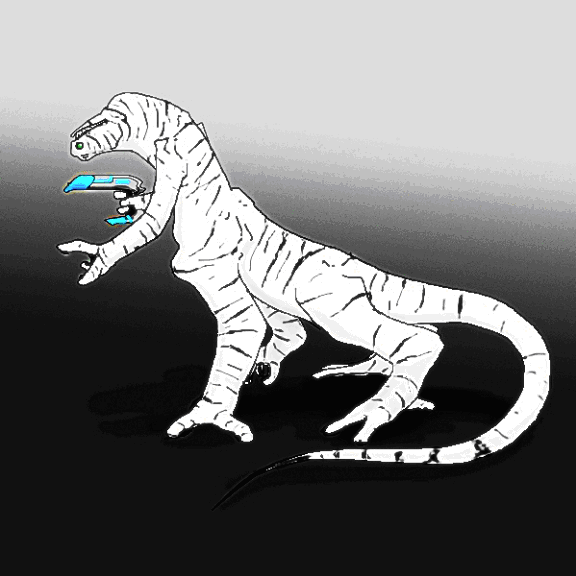
\includegraphics[width=\textwidth]{images/Aera.png}
}
    \caption{Aeran. Head is non-canonical and should treated as such. Rest of body is a reasonably solid depiction.}
    \label{fig:Aera-body}
\end{center}
\end{figure}


\subsection{Habitat}
The Aera homeworld was, prior to changes imposed by the technological
advancement of the Aera, a nearly seasonless planet with an
oxygen-nitrogen-neon atmosphere, on whose surface were a single large
landmass and many large and small islands. The mainland was nearly
entirely covered with jungles and marshgroves, with only small belts
of more sparsely overgrown land on the northern and southern reaches
of the continent. The rich jungle land was home to all sort and manner
of parasites, predators, diseases, and competitors for food. It was in
this vast, dark jungle that the Aera arose into sentience, tool use,
and civilization.

\subsection{Culture}
Aera culture is highly organized and decidedly hierarchical, but in
the form of a meritocracy rather than an aristocracy. While what has
constituted merit has morphed over the millennia since the first Aera
tribes selected work crews to cut back the encroachments of the jungle
upon their early settlements, given the relative position of the
pre-technological Aera in their local food chain, there has long been
a favoring of cleverness and determination over raw strength. The
current social and vocational position of any Aera is immediately
indicated by the color and pattern of an individual's coverall. The
Aera are ruled by a subset of the highest caste, with membership in
the oligarchy changing whenever either an individual steps down, or a
third of the other members call for a member's replacement. New
members must be confirmed by two thirds of the current oligarchy. It
is much more common for members to voluntarily remove themselves from
power, believing themselves more useful elsewhere in society, than to
be cast out. An average stay in the oligarchy lasts a few Aera years.

The long struggle of the Aera against the erosion of their society at
the hands of the natural world has instilled in them a deep respect
for that which has enabled them to conquer their environment:
technology. Not only is the advancement of technology greeted without
fear, the social position of the artificer and the engineer is one
more greatly elevated than that seen in any pre-Diaspora human
society. What is feared is the unmastered and uncontrolled. Even after
the last war between Aera and Aera was fought, bringing the last of
the major islands under the control of the mainland, the Aera only
slightly relaxed their military investment. Perhaps in large part due
to their short lifespan, and the consequential rapid dying off of
adherents to old theories, science advanced quickly, and with the
understanding of their place in the universe came a belief that just
as they had been forced to fight back against the jungle to keep
themselves alive, so would they likely have to push back against all
that waited for them beyond their world. Thus, eight centuries ago the
Aera burst forth from their homeworld, not afraid, but determined that
nothing would stand between them and their indefinite existence.

{\bf Factions and Organizational Groups}
Listed below are noteworthy Aeran sub-factions and organizational groups: 
\begin{itemize}
\item Aeran Merchant Marine
\end{itemize}

\subsection{Religion}
The nature of the Aera homeworld never inspired much belief in any
sort of loving deity. What began as a collection of local deities
coalesced, through conquest by what was to be the dominant group on
the entire planet, into a single pair of entites, one force of
creation, and one of destruction, both abstract, and both uncaring. As
time progressed, and the Aera advanced, these entities progressively
lost entity status and drifted into the realm of spiritual
concepts. Becoming more self-centered in their exploration of
existence, destruction morphed into personal death, and creation into
species survival. Organized religious activity among the Aera, such as
it was, ceased centuries ago, but the impact on their culture of the
concepts of death and survival is still quite strong. Indeed, Aeran
mausoleums are said to be, quite possibly, the only pieces of Aeran
art that might ever be considered beautiful. The Aera respect death,
but value is placed on the accomplishments made in the face of one's
imminent demise. All Aera are cremated, and the repositories for such
remains are vast public works, filled with displays of the
accomplishments of those entombed within, those who contributed
greatly to the species being rewarded with physical space devoted to
listing their deeds, and the rest consigned to a rotating schedule of
intermittent holograms and access via terminal displays. It is in such
places that an Aera would go to ponder, in silence and solitude,
relenting briefly from the near tireless schedule of a short-lived
species, the nature of its existence.

\subsection{Miscellaneous}
The Aera use a redundant numbering scheme:
Radix 3, digits drawn from the set of values {-2,-1,0,1,2} 

\section{Ancients}

\subsection{Physical characteristics}
There are precious few preserved remains of either species A or B
(especially B), so knowledge of their physiology is pieced together
from various, sometimes conflicting sources.

{\bf Species A}

Species A were moderately sized beings, between 1 - 3 meters in height, and no more than 2 meters in diameter. 

{\bf Species B}

Species B were smaller beings, no more than a meter wide, high, or thick. 


\subsection{Habitat}
The native habitats of these creatures are unknown. Given the nature
of the planets they settled, it can be assumed that they were
carbon-based lifeforms, and that at least of one of the two was an
oxygen breather.

\subsection{Culture}
Beyond their technological advancement, little is known. 

Excerpt from "A Brief History in Time and Space" 

"While there is much contention about the nature of the predecessors
of the Ancients, the Ancients themselves left enough rubble strewn
around the galactic arm to convince even a fairly hardened skeptic of
their having dwelled in these parts. The Ancients appear to have been
made up of at least two major species groups, and interacted with at
least three others, albeit it is not known whether these were client
species, or contemporaries from another part of the galaxy. Their
reign over this region lasted until about 1 to 2 million years ago,
whereupon they rapidly ceased to be present. There is a wealth of
evidence that severe infighting played some part in the destruction of
the Ancients, but, assuming there were victors in such a conflict,
little is known of what became of them.

The best source of such evidence, however limited, is the Uln
homeworld. While they are quite sensitive about the subject, the
widely held belief among the major races is that the Uln are the
descendants of the Ancient's equivalents of lab monkeys. The Uln
culture sprang up among the remains of a sprawling set of Ancient
structures... if they hadn't been so ill prepared for the gifts they
unintentionally received, they would have conquered the entire
arm. Fortunately for the aspirations of dominance held by other
species, the Uln were decidedly unprepared. Indeed, they spent so much
time blowing each other up with weapons they didn't entirely control
that it is a wonder that either they or the ruins on their planet
still survive.  The ruins, however, did not escape unscathed from the
genesis of the Uln culture. While assuredly the largest known source
of information on the Ancients, the ruins deliver little coherent
information about many key aspects of the Ancients' existences,
largely due to vast portions of many buildings having been turned to
dust."

To clarify, the statement about the Uln possibly having been able to
conquer the arm is contingent upon them NOT having blown most of the
ruins up, along with the devices they were using to blow each other
up, and large portions of their own species. No superweapons as such
are known to be currently possessed by the Uln. The Uln are in
possession of one particularly impressive piece of Ancient technology
(what is known as the Sul-Gatwa high castle), but it's potential is
effectively limited to the defense of their homeworld. However, even
as heavily damaged as the finds on the Uln world are, they remain the
best source for archeological research, and research visas remain a
large part of the Uln economy.

Why would this blasted planet be the best source of artifacts?
Because, unlike most of the planets that seem to have been inhabited
by the Ancients, it didn't have it's entire surface slagged, get
broken into a debris field of billions of pieces of rock, or become
pockmarked by craters implying assault equivalent to prolonged
planetary bombardment by 500Km wide asteroids.

Despite this, the occaisional piece of debris is found in such
places. However, the only officially reported finds of
fully-functioning Ancient technology have been the nano-plague and
various minor finds on the Uln homeworld.

The largest known piece of Ancient technology is the Sul-Gatwa high
castle. Whether or not it is technically functional is a matter of
some scholarly contention - the object is a slagged chunk of some
small moon sized ship or station. No systems appear to be remotely
functioning. However, what information has been declassified by the
Uln Royal Ingatwa fleet and confirmed via espionage implies that the
structure is so dense that it should have collapsed under its own
gravity into a solid mass - however, as the material that the high
castle is composed of defies the best efforts of science to explain or
duplicate (it has been jokingly dubbed "unobtainium") it could just be
some intrinsic property of the material and not evidence of
functioning gravitics. While the high castle has none of it's original
equipment and is, in essence a giant chuck of debris in orbit around
the Uln homeworld, every indication is that it retains the potential
to absorb absurd amounts of damage, and, as such, the centuries that
the Uln have spent arming it with their own weapons have made it the
most formidable planetary defense station known to exist. Its
existence, the threat of the Uln destroying what remains of the
Ancient artifacts, and general opinion that any of the major powers
could pen the Uln into their home system if necessary are believed to
be the primary factors responsible for the Uln remaining independant
entities.

Small fragments of Ancient technology, even completely non-functional,
fetch a fair price at any research facility or university
planet. Functional pieces of Ancient technology, even if relatively
useless, are of exceptional value, and it is not unheard of for
persons to attempt to make a career out of artifact prospecting,
subsisting on the rewards from finding small pieces of debris while
waiting for the big catch of working Ancient tech. However, as time
progresses, the easier pickings have already been scavenged, and
exploration of progressively more hostile environments has become
necessary to sustain the trickle of finds.

\section{Bzbr}

The Bzbr are a psuedo-reptilian species found on a jungle planet by
the Aera early in their expansion. The discovery of organized alien
intelligent life, even if harmless in it's neolithic state, furthered
Aera convictions about the dangers of the universe, even as they
worked to co-opt the Bzbr.

\subsection{Physical characteristics}
A Bzbr most closely resembles a jungle-green, copper-highlighted
1.5-meter long, ten-legged, arboreal reptilian with a nearly meter
long prehensile tail. Each limb has four segments, the fourth being
the hand/foot equivalent. The rear six legs are built for jumping, and
are used only for locomotion, the two underslung short arms primarily
for food manipulation, and the two forward inline limbs primarily for
gripping branches or other such objects, arching upwards and forward
from the rest of the body, in contrast to the other inline limbs,
which proceed upward and outward from the torso. Lacking vocal cords,
the Bzbr communicate in a simple language consisting of varied buzzing
tones produced by rubbing their feeder limbs together and motions of
the gripping limbs.

The Bzbr have three genders, breeder, broodherd, and
gatherer. Gatherers are the most common gender, and conduct all
hunting activities. Breeders are smaller than the gatherers, and
forage close to the nest area for roots and nest building material. In
far smaller number than the breeders or gatherers are the broodherds,
larger, stronger, sterile, and existing solely to protect the young
and territory of their sisters. Normal Bzbr nest groupings number in
the few dozens of adults. Bzbr are exceptionally short lived, living
only 35 - 40 years, even with modern medical technologies, but, given
their small size, this is not entirely unexpected.

\subsection{Habitat}
A world of jungle islands, spontaneous firestorms due to the high
oxygen content of the atmosphere, and extreme seasonal weather shifts,
the Bzbr homeworld can be safely considered unpleasant to all of the
known spacefaring races.

\subsection{Culture}
Adopted by the Aera out of some combination of pity and sympathy for
similar jungle origins, the Bzbr were pulled straight from the stone
age to the FTL age. Adapting about as well as can be expected to this
rapid change, many Bzbr simply went insane trying to adapt, but after
a few generations, the Bzbr had come to accept the new reality, even
if they were, due to rather much less than genius level average
intelligence, ill equipped to fully understand the full complexity of
it. Although not particularly bright or creative, the Bzbr are
actually quite good at both remembering and following instructions,
and have come to be used in various Aera space construction projects,
where they are valued for their ability to deftly maneuver in small
spaces and to leap from girder to girder. Bzbr, are, however, never
seen far from their Aera Patrons, as they are quite lost without
them. The Bzbr still, to some great degree, see the Aera as messengers
of the gods, having delivered them from the horrors of their world,
even if they know the Aera to be both mortal and fallible.

\subsection{Religion}
Though the Aera have attempted to convince them to do otherwise, the
Bzbr engage in hero-worship of the Aera. A majority of the Bzbr are
convinced that the actions taken in this universe play out in other
planes where the great nest of all life is threatened by chaos. They
believe that the Aera, by having brought greater order to their lives,
make them all great warriors in the other planes.

\subsection{Miscellaneous}
Bzbr use Aeran numbers. 

\section{Dgn}

The Dgn, like their brethren the Shmrn, are the descendants of a joint
Shaper and Lightbearer uplifting program begun with dextrous, tool
using, but pre-civilized saltwater marsh dwellers. The Dgn are the
branch cultivated by the Shapers and remain an integrated servant
class in Shaper society.

\subsection{Physical characteristics}
See images ~\ref{fig:Dgn-body} for bodyplan and ~\ref{fig:Dgn-motion} for locomotion (the Avian style is closest): 

\begin{figure}
\begin{center}
\makebox[\textwidth][c]{
    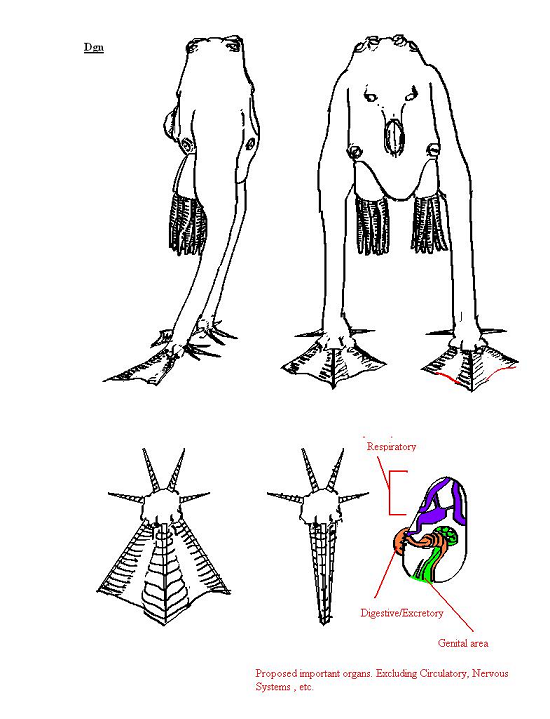
\includegraphics[width=\textwidth]{images/Dgn-body.png}
}
    \caption{Dgn body-plan}
    \label{fig:Dgn-body}
\end{center}
\end{figure}

\begin{figure}
\begin{center}
\makebox[\textwidth][c]{
    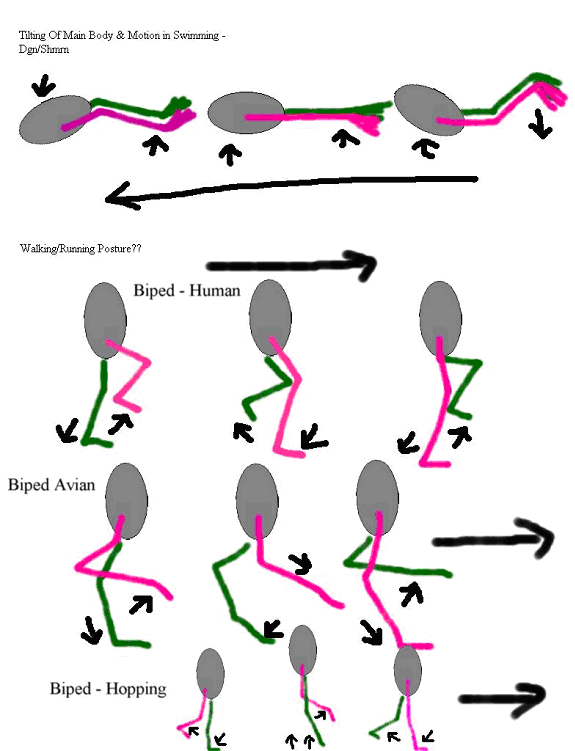
\includegraphics[width=\textwidth]{images/Dgn-motion.png}
}
    \caption{Dgn locomotion on land and in water}
    \label{fig:Dgn-motion}
\end{center}
\end{figure}



See Also: Shmrn (~\ref{subsec:Shmrn-species})

Through genetic engineering their life expectancy has been extended to over 50 years. 

\subsection{Habitat}

The Dgn can breathe in both atmospheric and aquatic conditions,
provided that there is sufficient oxygen dissolved in the water. They
do, however, require either a humid land environment, or frequent
re-wetting to keep both their skin and breathing orifices from drying
out. The native Dgn habitat ranged from coastal saltwater marsh-land
to tidal flats and into the coastal shallows themselves.

\subsection{Culture}

What native culture existed among the pre-modified Dgn has been
greatly altered. Bred for servitude, the Dgn are not greatly renowned
for intellectual achievements. The Dgn exist as a servant race for the
Shapers, working on nearly all Shaper aquatic projects, and filling
other unwanted roles in society. The one noted exception to this rule
is the use of Dgn as medical assistants in Shaper hospitals, where
their dexterity has proved them faster than humans at prepping the
injured for surgery. While the rights of the Dgn are well defined by
the Shapers, and abuse is not at all tolerated, their rights are not
the same as those of the Shapers, and if the Dgn are to be considered
citizens of the Shaper political body, then they are, at best, second
class citizens. The Shapers have built them to not be overly concerned
about this (the Shapers having had a different vision of what they
desired from their uplift than the Lightbearers, who were more
concerned with continued evidencing of their believed and beloved
superiority over lesser species). One cannot say that the Dgn are
entirely pleased with their position, but neither can one say that
there is fertile ground for revolt, as the Dgn do not seem to possess
within them a particular desire to be forced to decide their own
destinies. As the Dgn do not complain and the Shapers do not overtly
or actively seek to mistreat the Dgn, their freedom is something
sought after by activist groups rather than brought about by an armed
foreign entity.

\subsection{Religion}

Whatever glimmerings of disorganized religous beliefs they may have
had as more simple creatures have been lost. Currently prohibited from
engaging in organized religious activities due to historic fostering
of undesired solidarity.

\subsection{Miscellaneous}
Dgn use Human numbers. 

\section{Hoffman's blobs}

Hoffman's blobs are seemingly non-sentient creatures living in the
void of space. They were discovered by Burno Hoffman in the Barnard's
Star system.

\subsection{Physical characteristics}
Very little is known of those bizzare interstellar beings. The last
sighting has been in the Galileo system. Scientists are now flocking
to study these creatures before they leave, attempting to determine
how it is that they are able to sustain themselves in the void of
space. Observations suggest their size varying greatly, with the
largest individuals proving as large as a space cruiser, and the
smallest only the size of a shuttlecraft. It is uncleaer whether these
differences are attributable to age or polymorphism. The creatures
appear to primarily be drifters, but are capable of some acceleration.

\subsection{Habitat}
Hoffman's blobs live in the void of space. Since they were discovered
there have been six sightings of them, most recently in the Galileo
system.

\subsection{Culture}
There has not been any exhaustive research on the behavior of
Hoffman's blobs yet. From previous observations, it appears they
travel in flocks of about a dozen units.

\section{Humanity}

Table~\ref{table:relevantspecies} shows the relevant species in the UTCS time period and notes their organizational relations. FIXME (placeholder)

\begin{itemize}
\item	Homo Sapiens Sapiens (Faction with highest population percentage: Purists) 
\item	Homo Sapiens Superioris (Faction with highest population percentage: Shapers) 
\item	Homo Sapiens Cyberis (Faction with highest population percentage: Mechanists) 
\item	Homo Sapiens Pluralis (Faction with highest population percentage: Andolians) 
\item	Homo Sapiens Suprahomo (defunct) 
\item	Homo Sapiens Cosmonatalis (Faction with highest population percentage: Spaceborn) 
\end{itemize}
\subsection{Physical characteristics}
\begin{itemize}
\item Homo Sapiens Sapiens
\index{Homo Sapiens!Species info}
\index{Homo Sapiens!Homo Sapiens Sapiens}

Although small changes have occurred over the millenia, a great
percentage of the human population remains without intentional genetic
or physical modification, and thus remains not too far removed from
the humans of more ancient history. Whether through simple lack of
resources, lack of desire, or rejection of change, Homo Sapiens
Sapiens, unmodified except for the genetic drifts incurred over
centuries of colonization, remains the most populous of the human
subspecies.

\item Homo Sapiens Superioris
\index{Shaper!Species info}
\index{Homo Sapiens!Homo Sapiens Superioris|see {Shaper}}

Many eugenics programs have been launched in human history, but none
have been so successful. The path of self-affected evolution via
active genetic redesign has lead to a strain of humanity stronger,
more durable, more resistant to disease and injury, of higher average
intelligence, enjoying longer life-spans, and possessing keener
senses.  Assuming that the universally ink-black UV-resistant skin and
complete lack of any hair other than the signature blue-white
eye-brows is not disconcerting, any Superioris is almost certain to be
considered physically beautiful, but it takes some experience to
discern one Superioris from another. However, these benefits come at
the cost of much higher sustanence requirements, and a tremendous
narrowing of diversity.

\item Homo Sapiens Cyberis
\index{Mechanist!Species info}
\index{Homo Sapiens!Homo Sapiens Cyberis|see {Mechanist}}

Having replaced many of their body parts with mechanical equivalents,
or having forgone any pretense of human form, these cyborgs cover a
diverse and vibrant set of body types. Those with total body
replacement can usually pass anything short of close inspection if
they're willing to deal with maintenance of a synthetic flesh
exterior. If the goal is, as is often the case, to adapt the body to
the demands of work or habitat, anything from mining attachments to
full strength-enhancing endoskeletons could be an integral part of the
form. Locomotion seen to date ranges from bipedal to poly-pedal,
tracked, wheeled, or even sets of thrusters. In addition, this sort of
technical enhancement may provide the ability to extend one's lifespan
indefinitely if the base neurological systems have already been
altered to be non-senescent (provided one has access to regular
maintenance service). However, no matter how modified they may be, at
the least, portions of their brains and nervous systems remain.  While
communities of such modified humans exist on the worlds of many
factions, the Mechanist faction is the only full-fledged meme-group
centered upon the post-flesh goals of Homo Sapiens Cyberis.

\item Homo Sapiens Pluralis
\index{Andolian!Species info}
\index{Homo Sapiens!Homo Sapiens Pluralis|see{Andolian}}

While various communities have arisen that rely upon linked
existences, none save the Andolians have sufficiently differentiated
themselves en masse from the rest of humanity to be a discernable
grouping. Implanted at birth with hardware that allows data-net access
and an array of almost constantly transmitting sensors, a permanently
linked existence has rendered this strain of humanity notably
different in culture and mentality from all other strains.  While
every Pluralis retains its individuality, each is awash in a similarly
accessible sea of information. Culling from the group of those not
capable of entering into such an existence combined with a willingness
to engage in limited crafting of offspring has also lead to small but
noticeable genetic drift over the past 800 years. Implantation is
universal, and the use of synthetic or mechanically enhanced body
modifications is not uncommon, but the desire for total body
replacement present in the Cyberis strain is absent.  The linked
existence and general cultural proclivities of the Andolians have
brought them to near unity on their religious doctrine. While an
Andolian would refer to his/herself as a devout skeptic existing in
the absence of proof of the metaphysical, many others find it simpler
to call them Atheists.  While not overly concerned with improving the
physical form, health-related genetic traits deemed undesireable have
been recorded and then excised from the gene pool. When isolated for
long periods of time from any data-net, Pluralis individuals often
experience pronounced withdrawal symptoms, earning them the nickname
"Link-Junkies".

\item Homo Sapiens Suprahomo (Lightbearers) (Nearly Extinct) 
\index{Lightbearers!Species info}
\index{Homo Sapiens!Homo Sapiens Suprahomo|see {Lightbearers}}

One of the earlier factions to aggressively expand outward in the FTL
era were the Lightbearers, a meme-group built around the development
of a supra-human race. Believing the human form to be the sacred
forefront of evolution in the entire galaxy, they sought to claim the
place of their distilled and purified strain at the throne of all
sentients.

\item Homo Sapiens Cosmonatalis
\index{Spaceborn!Species info}
\index{Homo Sapiens!Homo Sapiens Cosmonatalis|see{Spaceborn}}

Crafted as a slave race by the now defunct Light-Bearer faction, the
Spaceborn, as they are commonly referred, remain frail and
over-specialized, incapable of surviving in planetary
environments. Instead, as they were designed, they spend their entire
lives in micro-gravity. The Spaceborn have a unique cardiovascular
system superbly tuned to life outside of a gravity well.  Their bone
structure, however, is a less cheery affair, and the Spaceborn, though
not suffering the degenerative effects of planetborn entities in
prolonged micro-gravity, never had much durability in the first place
and are weaker and more easily injured. They are almost universally
tall, lanky, and flexible, and all are possessed of a rather pallid
complexion tending toward a slight reddishness. Spaceborn frequently
begin developing severe medical problems between the age of 60-80
Earth years, giving them a somewhat shorter life expectancy than that
of the other subspecies.  Almost all Spaceborn live in habitats
situated in Andolian Protectorate space, having relocated from
Light-Bearer space after liberation from that faction.
\end{itemize}

\subsection{Habitat}

Originating on the third world of the Sol system, all variants of
humanity, even Homo Sapiens Cyberis, are most comfortable in
Oxygen-Nitrogen atmospheres, and temperatures not overly distant from
294 Kelvin.

\subsection{Culture}
Listed below are links to noteworthy human Meme-groups, organizations,
and governments:

FIXME 

\subsection{Religion}
Among the most mixed and varied in the known galaxy, running the gamut
from atheists to zealots. Refer to the individual groups for more
information.

\subsection{Miscellaneous}
Base 10. 

\section{Klk'k}
FIXME 

 
One of only five extant species to have achieved some measure of
space-flight prior to contact with other sentients, the Klk'k had what
can be readily argued as the worst first-contact experience on
record. Although the Andolian backed Ktah Restoration Project did much
to stem and repair the damage caused by the Lightbearers during their
occupation of Ktah, nearly a quarter of the Klk'k species were killed
by the Lightbearers, the majority of the deaths stemming from the
Lightbearers retargetting their fusion-tipped anti-orbital defense
missiles for ground impact and launching all batteries in a
scorched-earth response to the Hoshino Uprising. While the
laser-induced fusion warheads were exceptionally clean in the
radiologic sense, the scale of the bombardment was such that there
remain a number of areas of Ktah which have not fully recovered, even
at more than two centuries remove.

Currently, almost all Klk'k are citizens of the Andolian
Protectorate. While the Klk'k are self-governing over their own
colonies on domestic matters, with a government centered in Ktah, they
defer to the Andolians on external affairs. A significant minority of
the Klk'k population have become active adherents to the Andolian
meme-group, living integrated existences networked into surrounding
Andolian populations. Several mixed-species colonies featuring both
Humans and Klk'k exist, and there is both a human and Klk'k presence
on all Purth worlds.


\subsection{Physical characteristics}
average height range 4.5 to 5.5 feet (in meters?)

long, largish feet, reverse jointed knees, large easily splayed hips,
excellent jumpers, thick, disproportionally long, muscular legs in
proportion to generally much skinnier tops

wide, short, fair lengthed, back-bottom flanging head, with back
facing nostrils at the rear base between neck and jawbone

jaw is wider than head on each side. because of angle, more teeth on
bottom jaw than on top, bottom jaw teeth face slightly in, top jaw
teeth face slightly out

mouth contains 2 tongues. has no connection to air passageway. has
resonant "click" cavity in front top of mouth, behind and below the
rear of the bone ridges forming the eye sockets

eyes are large and wide set, and the sockets prononouced in their
bonyness

ears, such as they are, are 2 long curved ovoids, extending forward
from just behind and below the top of the jaw joint to somewhat even
with the top of the jaw joint and in front of the joint.  Mostly flush
with the skull, each ear is a series of cartilige-analog ridges
protruding slightly out from the side of the head to focus sound into
a central shallow curved trough, the bottom of which has numerous tiny
folds of hair-lined skin atop a drum

See additional discussion (later in document)

Figures ~\ref{fig:Klk'k-body-front},~\ref{fig:Klk'k-body-side}, and~\ref{fig:Klk'k-body-head} are poorly drawn sketches of the basic Klk'k body plan. Though
they show the general outlines, they are inconsistent as to whether
they are showing skeletal/muscular/etc. structures and details (to be
taken as rough guidance only - not canonical due to poor
implementation of desired visible outcomes (i.e. jacks can't draw
worth a damn))

\begin{figure}
\begin{center}
\makebox[\textwidth][c]{
    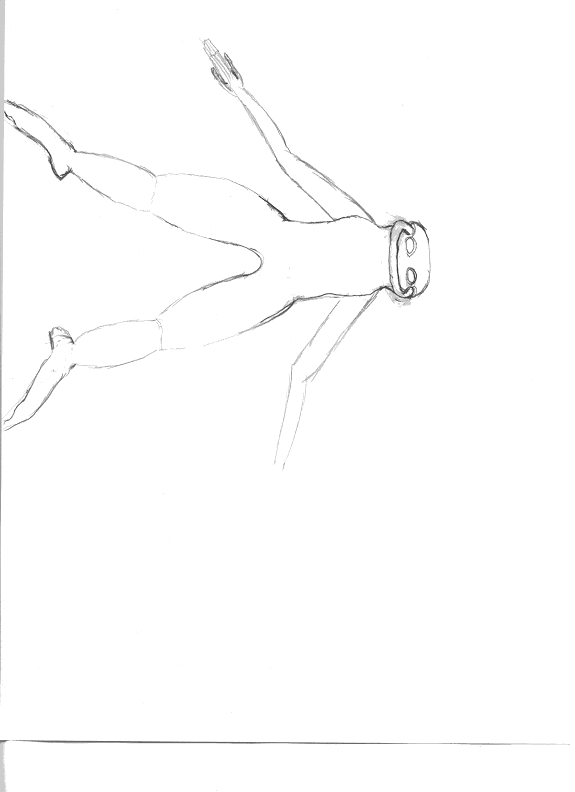
\includegraphics[width=0.75\textwidth]{images/Klk'k-bodyplan-front.png}
}
    \caption{Basic Klk'k body plan (front)}
    \label{fig:Klk'k-body-front}
\end{center}
\end{figure}
\begin{figure}
\begin{center}
\makebox[\textwidth][c]{
    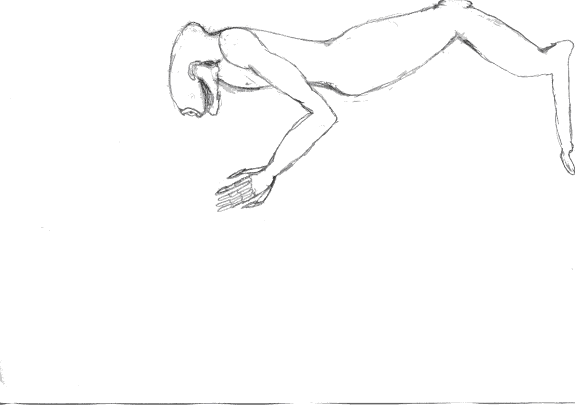
\includegraphics[width=\textwidth]{images/Klk'k-bodyplan-side.png}
}
    \caption{Basic Klk'k body plan (side)}
    \label{fig:Klk'k-body-side}
\end{center}
\end{figure}
\begin{figure}
\begin{center}
\makebox[\textwidth][c]{
    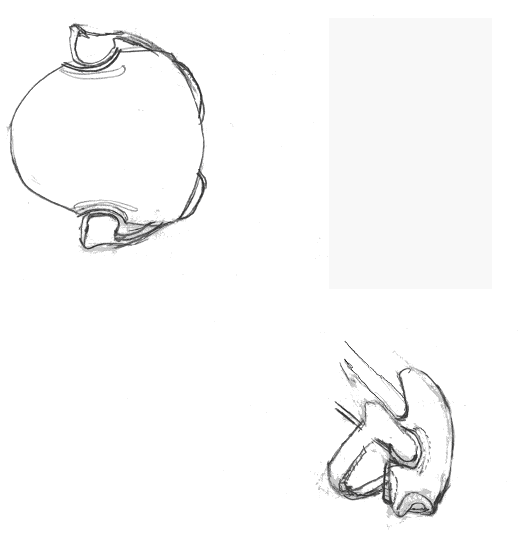
\includegraphics[width=\textwidth]{images/Klk'k-bodyplan-head.png}
}
    \caption{Basic skeletal structure of Klk'k head}
    \label{fig:Klk'k-body-head}
\end{center}
\end{figure}

The most anthropoid of the sentient species that humanity has
encountered (admittedly, two arms, two legs, two eyes, one head is
enough to place them ahead of most others), the Klk'k are nonetheless
notably alien in nature. Bipedal, with bilateral symmetry, the Klk'k
stand 1.3 to 1.5 meters tall on two splayed, reverse-jointed, muscular
legs, balancing on extremely elongated feet. Two arms,
disproportionately long by human standards, drape down from the
shoulders, each ending in a hand with four wiry fingers and two
thumbs, one on each side. The thumbs have something resembling nails,
while the rest of the fingers terminate with a hard, leathery, callus
covering the top and front, the finger-tips remaining fleshier. Klk'k
toes terminate in short, thick, blunt, stubby claws far more useful
for climbing than for tearing. The Klk'k head is wide and somewhat
squat in comparison to its breadth, being noticeably wider, at the
bottom, than the Klk'k neck. The Klk'k face features two large eyes
and a mouth that opens most of the way back to the jaw hinge. The
jawbone continues in an outward direction somewhat as it goes down
from the skull, further accentuating the width of the Klk'k head. The
Klk'k air passageways and digestive tract are separated. Breathing is
performed through two rear-facing nasal openings, one on each side of
the back of the head, situated behind and under the jawbone
attachment, opening where the head curves back to meet the neck. The
two eye sockets are protected by pronounced brow ridges. Inside the
mouth is a resonating click cavity, and two tongues. Klk'k have
several smaller, sharp, front teeth, and a smaller number of larger
grinding teeth, present only at the back of the mouth. Klk'k ears have
minimal external presence compared to human ears, presenting
themselves primarily as a furrow curving back and down along each side
of the Klk'k skull. The ears are water-tight, and Klk'k underwater
hearing is significantly superior to that of humans.

Klk'k are hairless, and the skin tends toward a swampy, uneven
green-brown, excepting the secondary sexual characteristics which
express themselves as thin, rosy-to-purplish highlights on the sides
of the head, hips, wrists, and ankles. Skin tends to be smooth, and
slightly leathery in texture, but a substantial layer of subcutaneous
fat keeps it from being hard to the touch. Both sexual and excretory
organs are positioned similarly to those of humans, at the posterior
of the torso. The Klk'k have two genders, the female of the species
tending to be the larger of the two, and distinguishable, among the
adult population, by the presence of more purple, rather than rosy,
highlights. Distinguishing between the genders of Klk'k children is a
more difficult task for the untrained human eye.

Klk'k have single fetus (with few exceptions) internal pregnancies,
and exceptionally long gestation periods. The later stages of the
pregnancy are extremely debilitating to the mother, eventually leaving
her nearly immobile as the fetus grows to increasing size and the
birthing blister migrates progressively closer to the
surface. However, at birth, the newborn Klk'k can already walk, swim,
and consume normal food.

Klk'k speech is produced primarily as a combination of vowels and
tones from the nasal airways and clicks from the tongues and
resonating chamber. Manipulation of the closures to the nasal airways
also produce a smaller number of consonants. The tonal nature of each
airway is independent, and harmonics have semantic and syntactic
meanings in most of the native Klk'k languages. The iconic Klk'k nasal
horn takes explicit advantage of the dual-tonal capabilities of the
Klk'k. Some human observers have likened Klk'k speech to listening to
a pair of Hawaiians having an animated conversation with a pair of
Khoisan, but most real xeno-linguists attempt to discourage such
simplistic comparisons as more misleading than informative. "Klk'k" is
itself an anthropic transliteration of their word for themselves,
likewise for Ktah, and Tk'latl, etc. As the Klk'k have proven far more
adept at understanding spoken human tongues, than the reverse, even if
they cannot produce the full range of human sounds, the anthropic
forms have become accepted standards, rather than requiring all humans
to utilize translator devices to refer to anything of Klk'k
origin. Klk'k living or traveling among humans tend to equip
themselves with vocalizing augmentation devices that fill in the
missing gaps in their ability to emulate human speech.

\subsection{Habitat}
Ktah is a warm, wet world with an Oxygen-Nitrogen atmosphere and vast
open stretches of ocean surrounding the two major continental
bodies. The Klk'k originated on the smaller of the two continents,
developing amidst the seemingly endless criss-cross of rivers and
bayous that dominate it. Though not amphibious, the Klk'k are quite at
home in the water, being excellent swimmers.

\subsection{Culture}
Humor plays a deep and intrinsic role in Klk'k culture, far beyond
that in any human one. While the Klk'k equivalents of humor and even
laughter have strong similarities to their human counterparts, the
situational appropriateness of humor is viewed quite
differently. There are few things that necessitate a somber decorum
for a Klk'k - they would see nothing inappropriate about joking and
laughing at someone's deathbed, funeral, execution, summit, board
meeting, intelligence briefing, etc. Indeed, quite the opposite is
true. Even war and combat are not seen as entirely serious realms --
there are numerous Klk'k stories involving tales of foes refraining
from death blows because each was waiting for the punchline of the
other's joke. Humor is also seen as appropriate in public actions,
officials, and governmental entities. In one particularly long-running
tradition, legislation is frequently put forward to change the Klk'k
anthem for the duration of a visiting dignitaries arrival in order to
make atrocious puns.

Being unable to find or generate humor in one's situation is a sign,
in a Klk'k, of a present or imminent psychosis, if often only a
temporary one. Klk'k can be riled to an indignant rage that, if short
lived, is still disturbing in its intensity. In Klk'k martial arts,
such as Amakakt, sparring contestants are often required to keep a
running dialog of humorous insults. If one of the combatants becomes
noticeably silent, the match is suspended, as it is a sign that
control has been lost, and the onset of rage may be approaching.

The basic Klk'k family unit is the the bond-set, based around a
mutually polyamorous clique arrangement. A bond-set usually consists
of 3-6 adult Klk'k and their assorted children, with the parentage of
the children coming from any arbitrary pairing within the
bond-set. Bond-sets consisting of only 2 Klk'k, save as a result of
the death of additional members, or as an initial state, are
considered strange, and their members potentially dysfunctional if
that arrangement persists. Bond-sets will continue to grow over time
by mutual interest in inclusion until they reach a steady point for
the individuals involved. Bond-sets with more than 6 members exist,
but are rare, as finding large numbers of co-interested partners is a
non-trivial task. Four members is the median expectation, and many
bond-sets of three partners will delay having children until a fourth
has joined. Some researchers believe the extended size of the basic
family unit to have roots stemming from the degree to which the later
stages of Klk'k pregnancies are completely incapacitating, leading to
a need for a larger supporting family unit.
\begin{itemize}
\item Bond-set Naming Conventions

The dominant culture for quite some time has used a strict two-name
scheme. When a bond-set is formed, the members choose a name for
themselves, and that is the bond-set name for those children raised by
that set. If the set changes, through addition, the name may be
changed or it may be kept, but the children will retain the old name,
unless very young. If the set changes through attrition, the name does
not change in order to honor what was, even if it is no more. One is
known by one's bond-set name (the name of those who raised you) and
your personal name, usually given in that order, thus Klk'k names are
not lineage tracing beyond a single generation.

\item Clothing and Ornamentation

Nudity was not a big deal in any notable pre-contact Klk'k culture,
and continues to be of little concern except among those Klk'k
visiting human worlds obsessed with particularly archaic
taboos. Common Klk'k coverings are as much practical and protective as
shielding from the public eye, featuring pockets, belts, places to put
or hang things, footwear, and isolated pieces to prevent scrapes and
scratches to various sensitive areas.

Klk'k style uni-gender semi-formalwear tends to be variants on a
loose, sleeveless (there is fabric straight from shoulder to neck, but
no collar), single-piece garment that runs completely flat across the
front, tapers slightly out from waist down and is slit in the back
somewhat below the end of the torso (the rear opening being convenient
for the Klk'k as their legs bend opposite those of
humans). Ornateness, except in extremely formal clothing, is highly
restrained, with patterns being limited to the edges and waist area,
running in thin seams around the garment. The prime regions of Ktah
are quite humid, and ostentatious layering would not have been
comfortable. Those looking for a more vibrant appearance tend to do so
with body paints on exposed skin rather than additional
clothing. Informal Klk'k clothing tends towards a short, loose skirt,
with tops, if any, varying by region.

There is also specific clothing to show respect, show allegiance, and
traditional body-paintings and tattoos. In particular, Amakakt tattoos
are expected among those practicing the martial art. A Tk'latl is
tattooed on the upper left topforearm/shoulder area, with annotations
denoting rank and record in Amakakt (the martial art heavily featuring
said Tk'latl). The ranking is above the Tk'latl, and consists of a
series of vertical bars of different color, denoting increasing ranks
attained, from left to right. A history of the matches is recorded in
colors corresponding to the rank of the opponents, and lies below the
Tk'latl, with vetical bars for victories and horizontal bars for
defeats.

Klk'k members of the Simons are known to frequently sport dynamic
tattoos, making their membership explicit when desired and hidden when
inconvenient.
\end{itemize}
\subsection{Religion}
The Klk'k frowned intensely upon organized religion even before they
settled under the wing of the Andolians. Klk'k history had been rife
enough with false prophecies and self serving church-like
establishments (including a theocracy that once dominated much of
Ktah) that the Klk'k analog to the Enlightenment had been rather total
in its sweeping reforms. Klk'k culture, however, has a long history of
veneration of ancestors, which continues in various ritualized forms
of behavior. There is no belief among the Klk'k that the deceased may
be contacted, nor is there any particular spiritual nature to the
reverence for those who came before, merely the conviction that it is
one's duty to honor the fact that, without them, one would not be.

\subsection{Miscellaneous}
Base 12, with numeral set derived from 2x2 entries in (2,3) double
base number system.

\section{Lmpl}

\subsection{Physical characteristics}
See Figure~\ref{fig:Lmpl} for image of a
Lmpl. Figure~\ref{fig:Lmpl-working} shows a Lmpl performing various
tasks.

\begin{figure}
\begin{center}
\makebox[\textwidth][c]{
    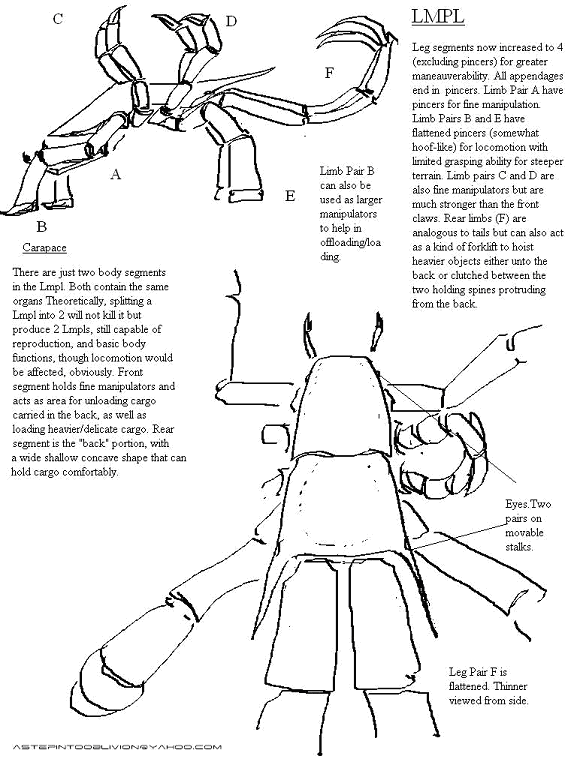
\includegraphics[width=0.75\textwidth]{images/Lmpl.png}
}
    \caption{Image of a Lmpl}
    \label{fig:Lmpl}
\end{center}
\end{figure}
\begin{figure}
\begin{center}
\makebox[\textwidth][c]{
    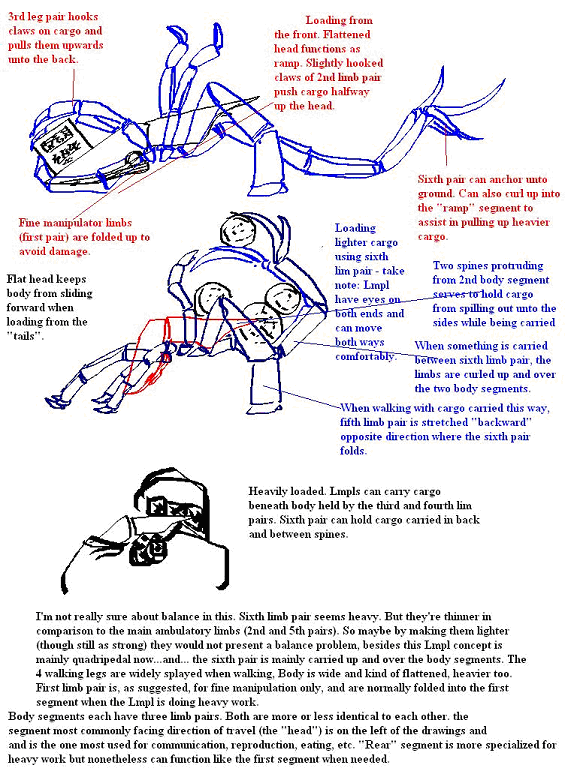
\includegraphics[width=0.75\textwidth]{images/Lmpl-working.png}
}
    \caption{Lmpl doing work}
    \label{fig:Lmpl-working}
\end{center}
\end{figure}


\subsection{Habitat}
Oxygen-Nitrogen 

\subsection{Culture}
Like the Nuhln, the Lmpl were a sub-sentient species that the Rlaan
selected for uplifting. The Lmpl were a project in adapting a lifeform
to an envioronment inhospitable to Rlaan workers. The Lmpl are
intelligent, but remarkably, and sometimes to a fault, single-minded,
though such is in keeping with their technical workforce mission. The
second of the two major uplift projects, the Lmpl are considered a
solid success, and enjoy their own niche role in Rlaan
society. Admittedly, as they are Oxygen-Nitrogen breathers, they spend
very little time actually in Rlaan society proper.

\subsection{Religion}
All Lmpl are adherents of Rlaanbzztkrlbzeentkaan (see ~\ref{Rlaanbzztkrlbzeentkaan}). 

\subsection{Miscellaneous}
The Lmpl use Rlaan numbers. 

\section{Mishtali}

The Mishtali were the first intelligent life forms Humanity came in
contact with, and at the time were enjoying a prolonged and happy
bronze age. Perhaps fortunately for them, the Unadorned were the
discovering faction, governing the Mishtali with a benign neglect. The
Mishtali managed the jump from a nomadic existence to being spaceport
baggage handlers quite well, all things considered, only eating a
fairly small number of colonists and tourists in the process.

\subsection{Physical characteristics}
See Figures~\ref{fig:Mishtali} and ~\ref{fig:Mishtali1} for details.

\begin{figure}
\begin{center}
\makebox[\textwidth][c]{
    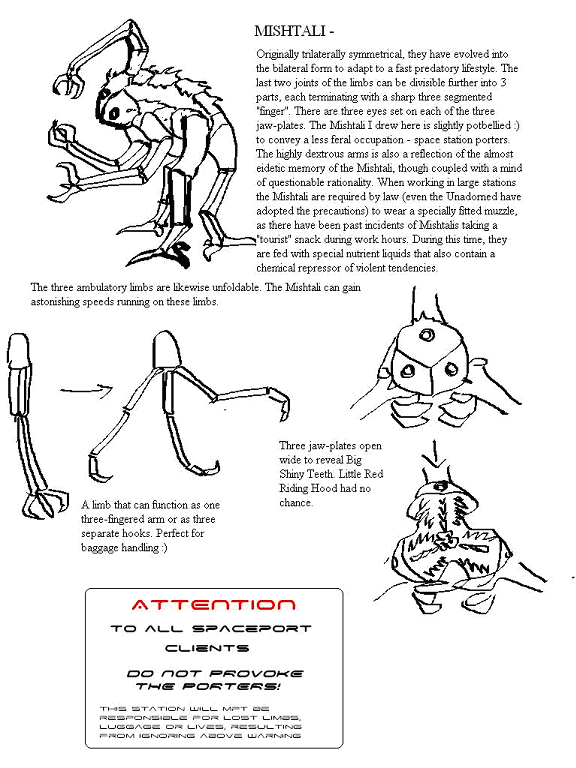
\includegraphics[width=0.75\textwidth]{images/Mishtali.png}
}
    \caption{Mishtali}
    \label{fig:Mishtali}
\end{center}
\end{figure}
\begin{figure}
\begin{center}
\makebox[\textwidth][c]{
    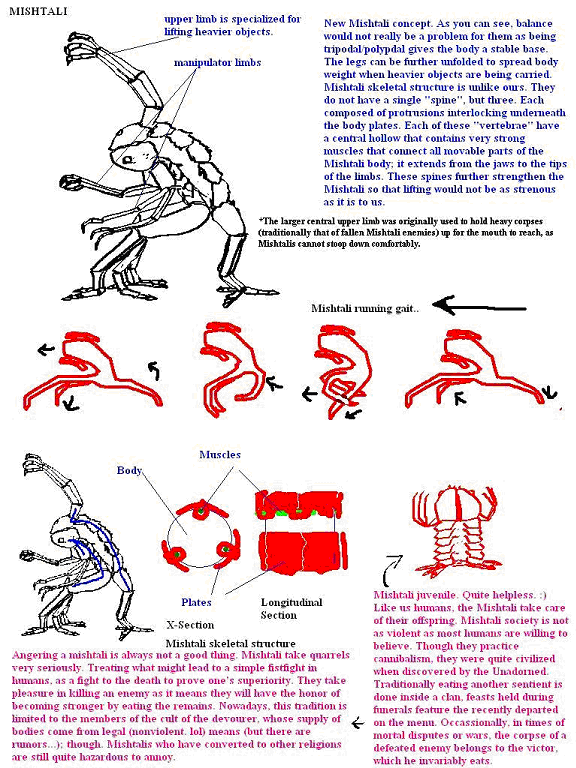
\includegraphics[width=0.75\textwidth]{images/Mishtali1.png}
}
    \caption{Mishtali}
    \label{fig:Mishtali1}
\end{center}
\end{figure}


\subsection{Habitat}
Oxygen-Nitrogen FIXME 

\subsection{Culture}
Given the cultural oddities of both the Unadorned, who come close to
religious reverence in their views on computers, and the Mishtali,
known for being the source of the Cult of the Devourer wherein the
religious rituals are accompanied by the consumption of the remains of
both Mishtali and alien sentients, it is believed by many to be just
as well that the Unadorned, as their discoverers, are responsible for
shepherding them.

\subsection{Religion}

The Mishtali practice a number of religions, both native and
foreign. Chief among the native religions in, albeit infamous,
notariety, is the Cult of the devourer. The Cult of the Devourer
centers on the belief that success in life is directly tied with what
one eats, and that the more powerful the being that was eaten, the
better one's life can be. Thus, eating the remains of sentient beings
is as good as it gets. This, obviously, raises a few issues among many
groups, but there are enough humans and Dgn willing to be paid for the
eventual consumption of their corpse that the churches of the Cult of
the Devourer tend not to lack for sustenance. These churches are, as a
rule, very festive and pleasant places to visit, provided one is not
turned off by the cuisine. The Mishtali have been very willing to
convert to just about anything, so the Mishtali also tend to have the
largest alien populations of most obscure human religions.

\subsection{Miscellaneous}
Base e.

This is what happens when math types (of admitedly questionable
initial sanity) decide to bring civilization to an undeveloped species
that doesn't understand exactly what is meant by "optimal".

\section{Nuhln}

\subsection{Physical characteristics}
Figure~\ref{fig:Nuhln} provides a clear depiction of a Nuhln.

\begin{figure}
\begin{center}
\makebox[\textwidth][c]{
    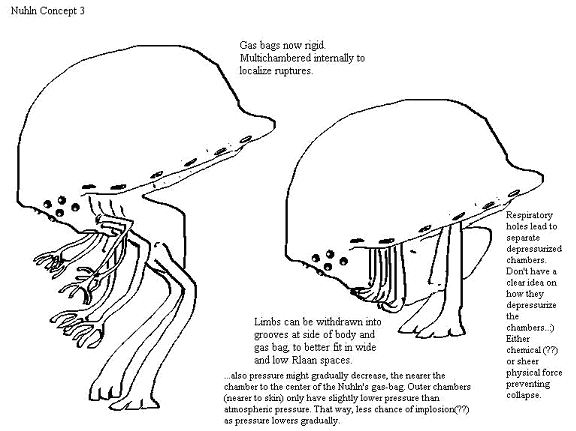
\includegraphics[width=\textwidth]{images/Nuhln.png}
}
    \caption{Image of a Nuhln}
    \label{fig:Nuhln}
\end{center}
\end{figure}

 
\subsection{Habitat}
Methane-Nitrogen 

\subsection{Culture}
Like the Lmpl, the Nuhln were a sub-sentient species selected by the
Rlaan for an uplift project. The first of the two major uplift
projects, the Nuhln are generally considered far less successful than
the Lmpl, being somewhat intellectually slow. They are almost
exclusively found performing jobs where the ability to repeatedly
perform seemingly mindless tasks without complaint is a distinct
positive attribute. Though present throughout Rlaan inhabited space,
they are a culturally subsumed group, possessing no internal culture
to speak of.

\subsection{Religion}
All Nuhln are adherents of Rlaanbzztkrlbzeentkaan (see ~\ref{Rlaanbzztkrlbzeentkaan}). 

\subsection{Miscellaneous}
The Nuhln use Rlaan numbers. 

\section{Purth}

The Purth are an uplifted client species of the Andolians. In large
part an experiment in synthesis of work done by the Unadorned and the
Mechanists, the Purth are cybernetic beings, with assistive AI and
built in networking capacity. It is only through these upgrades that a
Purth achieves something much like sentience.  Although they sometimes
operate autonomously from their Andolian patrons, Purth never do so
alone. Only by networking their minds together will a group of Purth
be confident enough to venture off without guidance.

\subsection{Physical characteristics}
The Purth were chosen primarily because of their very hardy
constitution, and have proved themselves invaluable in high gravity
applications. Each individual Purth is quite large, comparable to a
small motor vehicles, and covered in a skin heavily composed of
silicones. The silicones are at their most present on the footpads,
which allow the Purth to walk across still-cooling lava flows and
traverse boiling mineral springs.FIXME

\subsection{Habitat}
FIXME 

\subsection{Culture}
FIXME 

\subsection{Religion}
The Purth were pre-sentient before the Andolians altered them, and are
universally predisposed to ignore religious issues entirely.

\subsection{Miscellaneous}
Purth use binary, due to their number processing being heavily
computer assisted.

\section{Rlaan}

Ammonia-blooded, methane breathers from a cool world distantly
orbiting a hot star, the Rlaan are a collection of oddities. Unique
among the known space-faring groups, the Rlaan are actually two
separate species, the defenders and workers speciating some hundred
thousand or so years ago.

\subsection{Physical characteristics} 
{\em (Defender, Workers and Hybrids)}

Rlaan are radialy symmetric beings with a base four
split. Figure~\ref{fig:Rlaan-perspective} shows a perspective view of
a Rlaan from above. Their Workers (see
Figure~\ref{fig:Rlaan-worker-cutaway}) stand about one meter high at
the prime knee, and are nearly one meter in diameter. Members of their
Defender caste (see Figure~\ref{fig:Rlaan-defender-cutaway} for
cutaway image of Defender species) tend towards being 50\% larger in
both dimensions. Rlaan natively breathe a methane-based atmosphere,
and must wear special breathing apparatus to negotiate oxygen-nitrogen
environments. Their skeletal structure, being an exoskeletal carapace
supported internally by millions of reinforcing struts, is best suited
to lower gravity worlds, and leads to the use of mechanical assistance
on larger or denser rocky bodies.

\begin{figure}
\begin{center}
\makebox[\textwidth][c]{
    
\includegraphics[width=3in]{images/Rlaan-perspective.png}
}
    \caption{Rlaan - view from above and side}
    \label{fig:Rlaan-perspective}
\end{center}
\end{figure}
\begin{figure}
\begin{center}
\makebox[\textwidth][c]{
    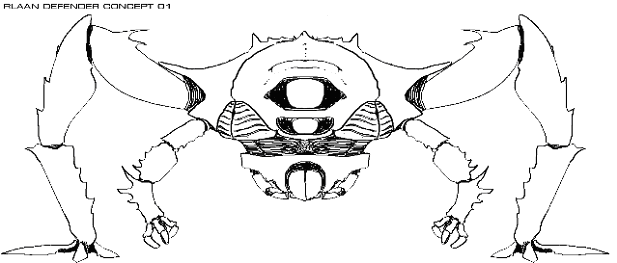
\includegraphics[width=\textwidth]{images/Rlaan-defender-cutaway.png}
}
    \caption{Rlaan Defender - front and back limbs omitted}
    \label{fig:Rlaan-defender-cutaway}
\end{center}
\end{figure}
\begin{figure}
\begin{center}
\makebox[\textwidth][c]{
    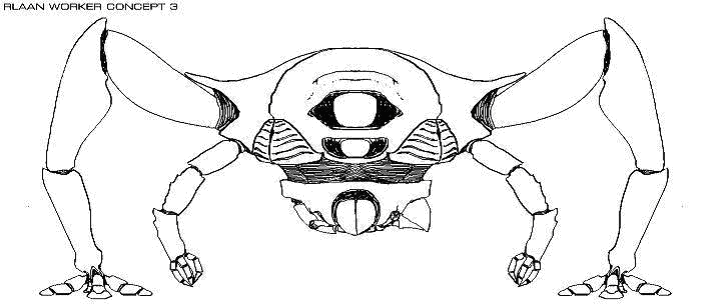
\includegraphics[width=\textwidth]{images/Rlaan-worker-cutaway.png}
}
    \caption{Rlaan Worker - front and back limbs omitted}
    \label{fig:Rlaan-worker-cutaway}
\end{center}
\end{figure}

Both species are similar in appearance, with the primary differences
being size, the degree of fine control in the manipulator appendages
(workers have better fine control), and the structural integrity of
the skeleton (defenders are less fragile than workers).  The defenders
tend towards darker shades of red and purple, whereas the workers are
somewhat pale. Though the offspring of worker-defender matings are
sterile, these hybrids exist as nearly 4\% of the population, and have
come to play important social roles, especially in the realm of
politics.  Rlaan are radially symmetric with four equivalent
segments. Each of these segments contains one compound eye composed of
four segments, one ambulatory appendage, one mouth with four
mandibles, one manipulator appendage, various local organs, and
portions of the central organs. The Rlaan skeleton is a supported
exoskeleton, that is to say, the exoskeleton is supported internally
by a network of millions of small extensions of the skeleton, which
together form a sort of highly porous lattice that the soft internals
reside in. A defender stands about 1.5 meters high at the top of its
carapace, and 2 meters high at its knee joint. The central body is
around one meter in diameter, and a third of a meter in thickness. Out
of this central body come the four abulatory limbs, going up and out
from the body to the knee joint, and then proceeding down where they
terminate in a four-splayed gripping foot. Suspended below the central
body is the "head" portion of the Rlaan, about half a meter in
diameter and also about a third of a meter in thickness, with its
bottom covered in a particularly thick extrusion of the
exoskeleton. The manipulator appendages sprout from the region
connecting the head with the main body, and end in four radially
arranged fingerlike structures. A worker's dimensions are about 70\%
that of a defender.

\subsection{Habitat}
With equatorial temperatures peaking near 230 K, seas of ammonia, and
a methane atmosphere, the Rlaan homeworld is not what most species
would consider a prime vacation spot. Life on this planet progresses
at a rather slower pace than that on water worlds, but proceeds
nonetheless. From the point of view of ammonia-methane life, the Rlaan
planet is actually quite toasty.

\subsection{Culture}
Rlaan lifespans tend to be between 250-350 years. This is believed to
be a large factor in their cultural homogeneity and the methodical
nature of their advances, both through space and as a culture. Rlaan
culture itself is a very dry affair, with social dynamics primarily
involved around expository investigations of philosophical debates
that have yet to be satisfactorily translated into the language of any
other species.

\subsubsection{Music}

Their music, if it can be called such, has been compared to "the set
of frequencies one would expect to register if a Myztherian Octpanther
were let loose in a campanile". On a more disturbing note, the Rlaan
central archives possess the largest collection of data concerning
Jerry Lewis and Yoko Ono outside of Human space. The Rlaan are,
however, regarded by many of the other space faring races as much more
intelligent than their culture's taste in art would suggest.

\subsubsection{Writing}

Rlaan written language appears as a sequence of characters consisting
of one to four radial slashes in each of four quadrants formed by a
pair of crossed lines. It is read in a counterclockwise spiral out
from a blank central region that is reserved for the signature glyphs
of the author. The Rlaan have vast stores of written documents going
back thousands of years, but attempts to decipher most of them have
met with limited success, as the concepts often being discussed seem
to have no corollaries in the languages of any other species.

\subsubsection{Science}

Rlaan science is more advanced in the fields of chemistry and genetic
manipulation than any of the other space-faring races. The Rlaan are
also quite knowledgeable about materials science and the advances in
the latter are often related to the former. Aside from these noted
cases though, Rlaan science has advanced more slowly than that of the
Humans or the Aera, and the extent of its advances is more a measure
of the age of Rlaan investigations into science than any particular
brilliance on the part of the Rlaan. Though not truly uncreative, the
Rlaan seem hard pressed in the department of inventive spontaneity. In
particular, the Rlaan are rather behind humanity in their exploration
of both artificial intelligence and tightly integrated biomechanical
systems, having sufficed with loosely coupled designer organisms.

\subsubsection{Politics}

The Rlaan are governed by a body whose name translates to The Rlaan
Assembly it appears to be some form of representative democracy, but
the exact methods of choosing one's representative seem complex and
arcane beyond the tolerance of most observers to bother attempting to
figure out. This body then churns out laws and regulations at a
breakneck pace, the enforcement of which is then delegated to the
complex Rlaan Bureaucracy. Attempts to understand the inner workings
of the Rlaan Bureaucracy have met only with confusion for all parties
involved. Strangely, the members of the Assembly are
disproportionately sterile hybrids, believed by the Rlaan to be more
levelheaded than either the aggressive defenders or the timid
workers. One thing that did translate clearly, however, was the Rlaan
differentiation between civilian and non-civilian. Given their
biological distinction between these two, it is easy to see why the
Rlaan have such firm views upon how civilians should be treated.

Notable Rlaan Factions and Organizational Entities
\begin{itemize}
\item The Rlaan Assembly 
\item Rlaan Briin 
\item Rlaan Merchants 
\item Rlaan Hunters 
\item Rlaan Enforcers 
\end{itemize}
\subsection{Religion}
\label{Rlaanbzztkrlbzeentkaan}
Most Rlaan are adherents of Rlaanbzztkrlbzeentkaan. What this means is
very difficult to say, as, though it is a text based religion, the
text is under constant revision. Indeed, the Rlaan Assembly regularly
submits changes and additions to the holy text. Contradictory edicts
abound, and scores of companion volumes are included with every copy
that debate the relative merits of breaking one set of edicts over
another. Edicts contradicting each other,however, are the least of a
reader's worries, as the universe is created 37 times in 17 entirely
distinct fashions, by a grand total of 4301 entities, albeit 4210 of
these were all in one creation story. History, morality, ethics, and
the fundamental nature of reality itself are all presented in so many
different forms in the text, that it defies rational understanding as
to how the Rlaan consider the book canonical and relevant. However,
they do. And they gather together at one of the 73 specified intervals
of worship, for those that interpret worship as being allowed, to
engage in whatever activity is currently believed to be both correct
and legal by the group that has thus met. Rlaan places of worship are
thus remarkably like most Rlaan art: constantly changing in nature but
composed of themes that are themselves mind-numbingly repetitive, and
constantly possessed of an aesthetic that runs counter to common human
tastes.

\subsection{Miscellaneous}
Depending on your viewpoint, the Rlaan use either base 4 or base
256. Namely, every Rlaan character is composed of 4 subcharacters, so,
going by the subcharacters, it's base 4, but there are 256 distinct
numerals per character read. Rlaan numbers are distinguishable from
the characters in the rest of the Rlaan script in that the center of
each subcharacter is marked with a dot. As far as the Rlaan are
concerned, it's base 256.

\section{Saahasayaay}

Fast, beautiful and deadly, while they serve the Rlaan, they do so
because of the technological and economic benefits gained from the
association rather than out of gratitude. Whereas the Rlaan succeeded
in making both the Lmpl and Nuhln useful and docile, the Saahasayaay
are indeed useful, but far from docile.

While the Saahasayaay are a single species in the technical sense,
their array of different metamorphic forms, each clearly of distinct
origins, is somewhat unique, and, as only certain of the forms are
possessed of any particular intelligence, and only one of accepted
sapience, in common reference "Saahasayaay" may often refer only to
the portion of the population in dominant sentient morphology.

The Saahasayaay have the strangest, and, on several levels, most
disturbing life cycle of any of the known extant sentients. Foremost
among its disturbing points is that the life cycle is clearly of
artificial origin external to the Saahasayaay homeworld. The
non-squeamish often find this more disturbing than the fact that
metamorphosis usually begins with the death of much of the body, and
proceeds via the semi-autonomous archival organ consuming what would
otherwise be the uneaten remnants of its own corpse to fuel its
generation of a new body. The archival organ, itself effectively
inedible, and encased in a protective shell, is not a native
feature. The organ features an absurd amount of unexpressed genetic
code - indeed, it contains genes describing thousands of species,
almost none of which are actually present on the Saahasayaay
homeworld. Indeed, the Saahasayaay appear to be the result of some
ancient (although not believed Ancient) xenoforming gone awry. Many of
the gene sequences present in the archival organ appear to be
irrevocably damaged or woefully incomplete, despite the presence of
significant error correcting facilities.

Only the lowest level of the metamorphic chain for the Saahasayaay can
actually breed. All other forms have been rendered sterile. This
lowest level is a fast growing photosynthetic invader species that has
infiltrated or replaced competitors in most of the native ecosystems
of the Saahasayaay planet. It cannot be correctly termed a plant,
animal, or fungus, although it shares some features with all of these
more familiar categories. While likely originally designed to be the
prime xenoforming agent for the planet, destroying native ecosystems
and replacing them with those of its creators, the archive creeper has
wandered from its original mission, producing a warped hybrid
ecosystem that almost certainly bears little resemblance to either the
original or intended replacement. The origins of the Saahasayaay are
clear in both their metamorphic paths, their traditional food chains,
and the sterility and monosexual nature of all of the extant forms
save for the archival creeper. Local "herbivores", for lack of a
better word, came to eat the creepers, but were in turn recorded and
replaced, themselves devoured and recreated by the archival organs
they attempted to consume. This effect then proceeded to trickle up
the food-chains of all of the ecosystems invaded by the creepers. A
limitation of this process, was, of course, that organisms smaller
than the archival organ were not readily assimilated. Thus, the
detritus feeders competing for flesh on the fallen corpse of an
assimilated species were more likely eaten by the archival organ than
the other way around.

The archival organ is an incredibly complex, advanced, and subtly
broken biological machine, but it is not itself remotely
intelligent. Likewise, it is not quite sufficiently autonomous to
generate widespread agreement as to it being referred to as a
symbiotic organism, especially as the genetic definitions are skewed,
given that it contains all of the genetic code for all of the "host"
bodies. All tissues in the archival organ feature cellular
immortality, and the archival organ is itself amortal (not aging, nor
dying from old age) although the bodies it produces do not share these
properties. The organ is well protected and possesses some independent
subsystems, so surviving the death of the rest of the body is common
(depending on the manner of host-death) - which is necessary, given
that such is the only means for morphological change and the
preservation of more interesting forms of species. The archival organ
plays key hormonal regulatory roles in all of the assimilated forms.

\subsection{Physical characteristics}
Terminal form Saahasayaay are physically impressive beings, if not,
because of mode of movement, as bulky as some of the other sapients,
and fossil records indicate this to be a quality preserved from
pre-assimilation times. They are beautiful, if possessed of features
that, if designed, would speak of a certain viciousness to the
crafting hand. The terminal Saahasayaay are the only extant sophonts
known to be able to fly, albeit they are, in practice, more often
gliders than active flyers through their thick and caustic
chlorine-nitrogen atmosphere. Their bodies are long, almost
serpentine, though the strong muscular development for the wings and
arms belies that image. They are bilaterally symmetric, with 4 wings
rising above, and 8 arms hanging below the largest and middlemost
segment of the body, set between a long tail at rear and longish neck
and fierce head at front. The front and rear sets of arms have
hand-like endings, gripping appendages of a gaunt leather-and-bone
appearance, that are dexterous, if clearly meant to hold fast to live
and struggling prey while the curved blade-like endings of the middle
four arms carved and scooped the meal into edible submission. Skin on
the middle-body is mostly hidden behind large, thin, overlapping
scale-like protrusions of smooth, hardened flesh, iridescent, ranging
through colors from green to red to gold. The tail, in cross section,
could be thought of as a square whose sides have been bent in, or
whose corners were pulled out, to produce a four-sided concave
shape. The tail is heavily segmented, as is the neck, which has a
similar shape, although much larger, and it lacks the short spines
protruding from the corners of each tail segment that serve to let the
tail be used to grip surfaces or objects it has been wrapped
around. The tail narrows somewhat as it progresses rearwards, but was
always fairly thin in comparison with the body. Towards the rear of
the tail, the spines end, and four specialized spines are present that
act as fins that can be raised or lowered to act as flight control
surfaces. The scale-like protrusions are much larger on the tail and
neck than on the body, corresponding heavily to the structure of the
segments themselves leaning somewhat towards a more chitinous-plates
appearance than scale-like appearance, for those portions, although in
truth it is only a matter of size and flexibility required for each
segment that has lead to the differing appearance, and not a
fundamental change in material. The head is slightly larger in girth
than the neck, excepting the mouth itself which is forward of the rest
of the head. The terminal form Saahasayaay have no teeth in their
mouth. Grinding, separating and pulverizing are instead done by
stone-hard protrusions that line their equivalent of the
esophagus. The mouth instead consists of a set of flexible, segmented
spines, connected to each other by membranes, that can be focused to a
point, as when sucking in fluids or flying, or opened to engulf a
portion of a prey animal. This semi-engulfing is necessary, as the
chunks of flesh freed from the target by the multiple bone-bladed
tongues that slash out violently from within the mouth might otherwise
fall out. There are four eyes, two at the corners of the top of the
head and two, more centered, below. There are ears and nasal openings
that lie on the side of the head. The brain itself is primarily on the
top of the head, although there is significant neural matter at the
bottom of the head that does optical processing for the lower eyes.


\subsection{Habitat}
All of the native species integrated by the archival organ are now
extinct. Thus, entire food-chains now consist of nominally Saahasayaay
organisms. It is presumed, given that all of the non-creeper
morphologies are sterile, that the intended process involved a
kill-off of all of the food-chains via a wave of progressive
morphology changes up the food-chain, thereby progressively starving
each link in the chain. Alternate theories presume an external agent
being introduced that would kill off all of the hybridized life forms,
while leaving the invaders intact, but the non-native codes are
sufficiently mangled that it has been difficult to test if such
differentiation would have been readily achievable. Given the large
number of codes stored, it is presumed that total kill-off was not an
intended goal. Clearly, however, none of these have happened,
especially those models requiring external intervention. Instead, the
regulatory mechanisms presumably in place to delay any native
depopulation until there has been sufficient infiltration of the
native populations have instead functioned merely to regulate the
frequency with which the next body of a dead Saahasayaay differs from
the previous. Also noteworthy is the terminal nature of the
Saahasayaay metamorphic process. Fossil records point to the ancestor
of whatever native species preceded the sapient Saahasayaay population
as having been wide-ranging, and wherever present, atop the food
chain. Thus, the Saahasayaay sophonts are currently the "terminal"
metamorphic form - an archival organ that survives a Saahasayaay
sapient's death will normally build another Saahasayaay sapient. Note
that none of the previous individual's memory or mentality is
preserved, and inefficiencies in conversion and the genetic
imperatives of brain development in the original source species, even
in the presence of a nearly full corpse, result in the production of a
juvenile individual.


\subsection{Culture}

The most successful of the Rlaan client species, the Saahasayaay are
not, unlike the Nuhln and Lmpl, true uplifts, having already achieved
some minimal level of societal advancement at the point of discovery.

The Rlaan have taken to using Saahasayaay troops to reinforce their
border with the Aera, are, however, somewhat hesitant to let this
concentration of troops return home.

As most of the Saahasayaay forms are not capable of complex thought,
they don't much consider either the nature of their life cycle, nor
that they often are eating what is technically a member of their own
species. This is not the case for terminal form, whose culture has
been deeply shaped by the role that death plays in the Saahasayaay
life-cycle, and the semi-reincarnations that are the daily occurrences
of Saahasayaay life. The terminal form Saahasayaay are, in fact, quite
bright, and learn voraciously, but a cultural disinterest in knowledge
unrelated to superior killing ability and an exceptionally low
life-expectancy rate due to unending war, murder, and ritual killings
has historically hampered internal sources of advancement. It is not
too difficult to see where their obsession with death has come from,
albeit only they, perhaps, can truly comprehend the directions it has
taken them in. It is fortunate for all other sapient species in the
region that the Saahasayaay were found in the stone-age by
space-faring sapients, and not the other way around, as the
Saahasayaay have no compunction when it comes to killing, whether it
be other sentients, each other, or lower Saahasayaay forms. Death is
the natural order for them, it is the source of progress, and their
right and duty to disperse. Their obedience to the Rlaan and restraint
in aggression against both the Rlaan and other species is predicated
on the Rlaan's greater ability to bring death upon them than they upon
the Rlaan, as well as the opportunity for greater empowerment that the
Rlaan bring to the Saahasayaay. Death is the ultimate blessing the
Saahasayaay believe they can bestow, and the frequent regeneration of
their fallen into newborns has utterly deprived them of the fear of
their own demise present in all other known organized species of
measurable intelligence.

Some of the other Saahasayaay forms possess some level of
intelligence, though none as pronounced as the terminal form
Saahasayaay. Some of these forms have been "domesticated" and the most
intelligent of these, generally considered comparable to some of the
Terran primates, are sometimes used in a servitor role. The most
valued of the servitors are granted a chance at "ascension" by being
taken to an isolated area, free of terminal Saahasayaay, and killed
swiftly, leaving the entire corpse intact. The lack of terminal
Saahasayaay in the area improves the likelihood that the next
metamorphic form will be a terminal Saahasayaay, rather than another
servitor, as the choice of next form is heavily influenced by the
presence of other forms detected by the archival organ, a
manifestation of its original, more overarching regulatory
role. Punishment in terminal Saahasayaay society rarely involves
killing of the archival organ, an act considered disgraceful unless
the individual in question has been deemed to be heretical to the
advancement of the Death God's agenda, but it almost universally
involves killing. Punishments range from the minor, a swift and clean
death followed by adoption for what most other species would consider
misdemeanors, to use as hunt bait and eventual consumption by lower
forms, to the most serious crimes being punished by the removal of the
archival organ, the starvation thereof for a period of time, to
increase the chance of form reversion, smearing the archival organ in
the mixed remains of lower forms to further increase the odds that the
next form will not be a terminal Saahasayaay, and then letting the
starving archival organ eat the victim (still conscious, but wracked
with crippling chemical imbalances) alive.

It is generally considered fortunate that only a small percentage of
the world known to be reachable via the jump network feature a
chlorine based ecology. The Saahasayaay, from the creeper on up,
feature a profoundly rapid metabolism, and they have quickly overrun
and populated other chlorine-worlds that they have been introduced
to. Indeed, it has long perplexed researchers as to why exactly the
concentration of chlorine-life friendly worlds is significantly higher
in the region of space containing the Saahasayaay homeworld, and then
marginal elsewhere. What many believe to be the likely originating
planet of the archive creeper is in very nearby space, just one jump
link removed from the Saahasayaay system, but it is difficult to
ascertain this connection with any certainty. The system shows signs
of previous habitation by a technological entity, but, outside of
semi-preserved ruins on various moons and other uninhabitable
locations, there is precious little left of the inhabitants. In
particular, what is believed to have been their homeworld would seem
to have fallen victim to both some sort of limited grey-goo event and
a widespread use of fusion, antimatter, and kinetic weapons that,
combined with the already reactive nature of the atmosphere, served to
make it exceptionally difficult to discern much about the previous
inhabitants. Levels of nano-plague are also exceptionally high in the
system, leading several researchers to advance theories that the
inhabitants made what proved to be a fatal mistake of attempting to
counter the nano-plague in an aggressively military fashion.

The Saahasayaay navigate 3D space with great agility, and, despite the
distinctly different dynamics of planetary and vacuum flight, make
excellent pilots in either medium. The Saahasayaay have not
significantly industrialized on their own, although their
technological usage has greatly advanced since absorption into the
Rlaan Assembly. All Saahasayaay ships are specially manufactured for
them by the Rlaan out-system, and Saahasayaay pilots shipped out to
military bases from one of the Saahasayaay worlds. The Rlaan are
somewhat reticent when it comes to providing the Saahasayaay with a
means to make their own starships. They are, however, more than
willing to freely give them technologies which increase their
sustainable populations so that they can draw upon more Saahasayaay
troops. The Saahasayaay, for their part, hunger for more control over
their own destiny, but are currently kept sated with the opportunity
to bestow much bigger deaths with the starships the Rlaan build for
them (the Saahasayaay consulting on certain aspects of the
design). Saahasayaay operating in Rlaan space must wear
atmosphere/temperature suits at all times, precluding flight
abilities. Their suits are therefore augmented with thrusters so as to
make them more comfortable - an uncomfortable Saahasayaay is not a
safe Saahasayaay, though there is of course, no such thing to begin
with. Saahasayaay work only with defenders and hybrids in Rlaan
society. They have no respect for the Rlaan workers, who cannot be
killers in any meaningful way, and the Saahasayaay are considered an
unnecessary threat in interacting with Rlaan workers.

\subsection{Religion}
The dominant belief structure of the Saahasayaay revolves around each
of them being an intruments of the great death god who sits in
judgment over the universe. The Saahasayaay belive themselves to be
the chosen people who alone are privy to the sentences being passed
down upon the mortals of this realm. Saahasayaay prophet halls are
built to express the joy of the hunt, the glory of the kill, and
subserviance to the great death god. The prophet halls are built in
keeping with the 3-dimensional nature of Saahasayaay travel, with
perches on many levels, and rank denoted by attainment of a higher
perch.

\subsection{Miscellaneous}
The Saahasayaay used to use a unary system with groupings done in sets
of 8 (flat, without a notion of base), but have been converted to use
of the Rlaan base 256 system.

\section{Shmrn}
\label{subsec:Shmrn-species}
The Dgn and Shmrn share a common time-of-uplift ancestor. The
resulting species was further refined in seperate efforts by the
Lightbearers and the Shapers into two distinct, but closely related
species. As the Lightbearers were destroyed as a meaningful entity,
the Shmrn were let loose as a freed species to settle new worlds.

\subsection{Physical characteristics}

\subsection{Habitat}

\subsection{Culture}

For above 3 categories, please see the following list of images: Figures \ref{fig:Shmrn-overview}, \ref{fig:Shmrn-ancestral}, \ref{fig:Shmrn-elder}, \ref{fig:Shmrn-medic}, \ref{fig:Shmrn-pilot}, \ref{fig:Shmrn-pilot1}, \ref{fig:Shmrn-footwear}, \ref{fig:Shmrn-formalwear}, \ref{fig:Shmrn-logo}, and \ref{fig:Shmrn-render}.

\begin{figure}
\begin{center}
\makebox[\textwidth][c]{
    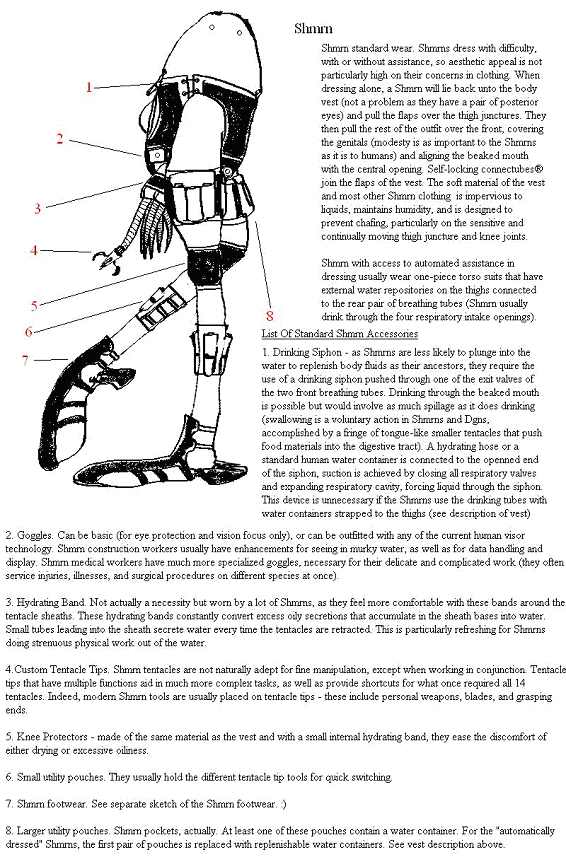
\includegraphics[width=0.75\textwidth]{images/Shmrn-overview.png}
}
    \caption{Shmrn Overview}
    \label{fig:Shmrn-overview}
\end{center}
\end{figure}
\begin{figure}
\begin{center}
\makebox[\textwidth][c]{
    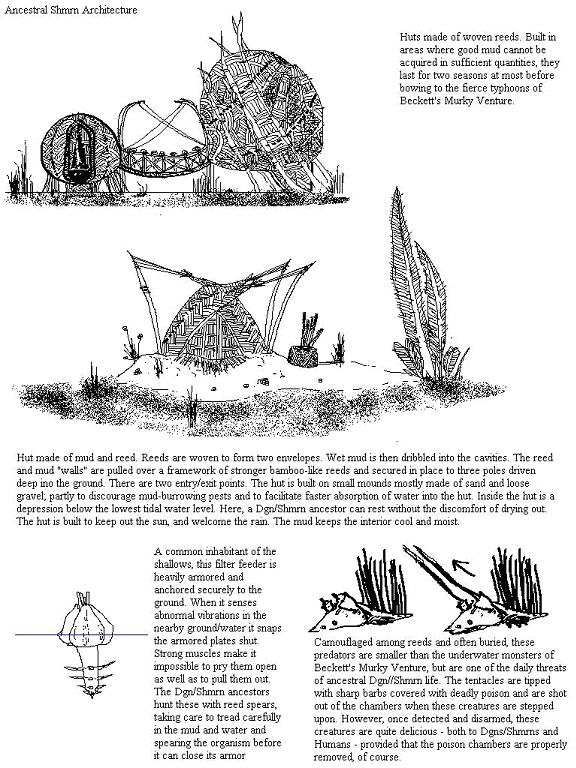
\includegraphics[width=0.75\textwidth]{images/AncestralShmrnArchitecture.png}
}
    \caption{Habitat of the ancestral Dgn/Shmrn}
    \label{fig:Shmrn-ancestral}
\end{center}
\end{figure}
\begin{figure}
\begin{center}
\makebox[\textwidth][c]{
    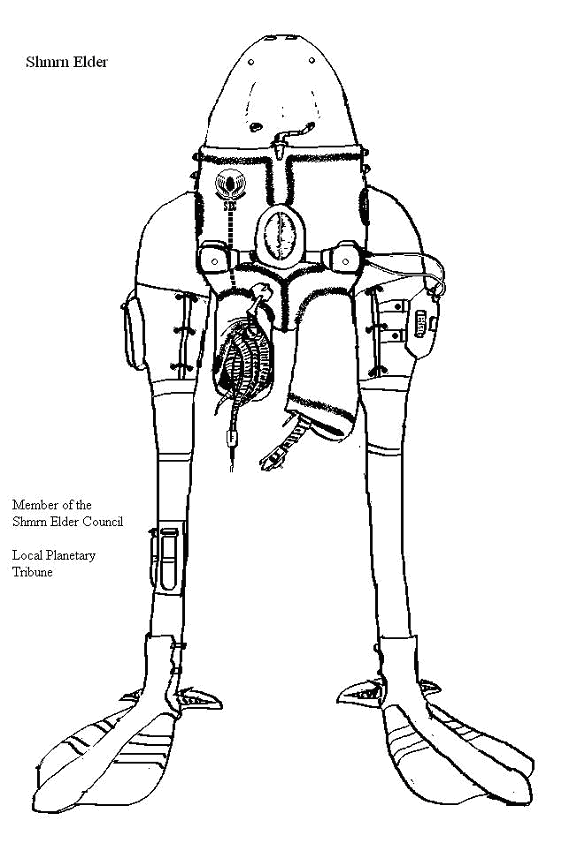
\includegraphics[width=0.75\textwidth]{images/Shmrn-elder.png}
}
    \caption{Shmrn Elder}
    \label{fig:Shmrn-elder}
\end{center}
\end{figure}
\begin{figure}
\begin{center}
\makebox[\textwidth][c]{
    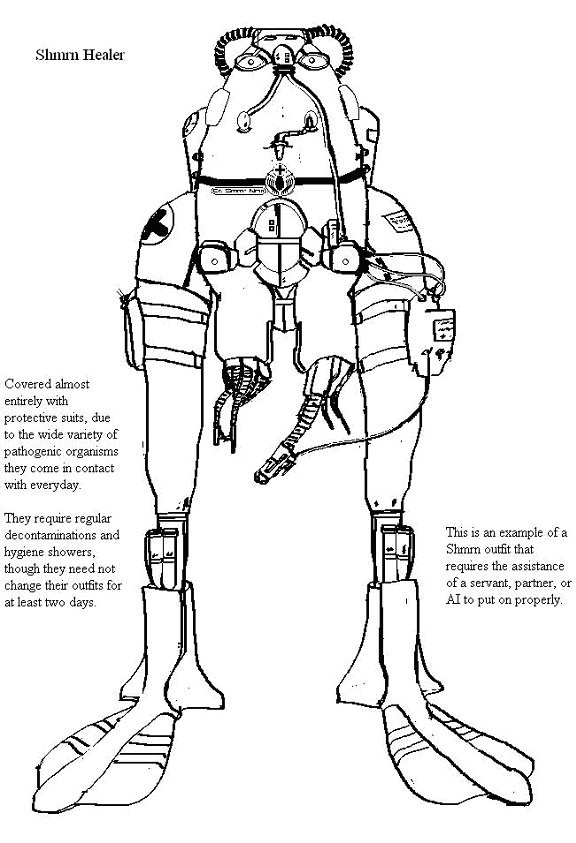
\includegraphics[width=0.75\textwidth]{images/Shmrn-medic.png}
}
    \caption{Shmrn Medic}
    \label{fig:Shmrn-medic}
\end{center}
\end{figure}
\begin{figure}
\begin{center}
\makebox[\textwidth][c]{
    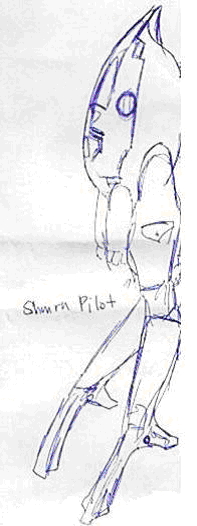
\includegraphics[width=0.25\textwidth]{images/Shmrn-pilot.png}
}
    \caption{Shmrn Pilot(1)}
    \label{fig:Shmrn-pilot}
\end{center}
\end{figure}
\begin{figure}
\begin{center}
\makebox[\textwidth][c]{
    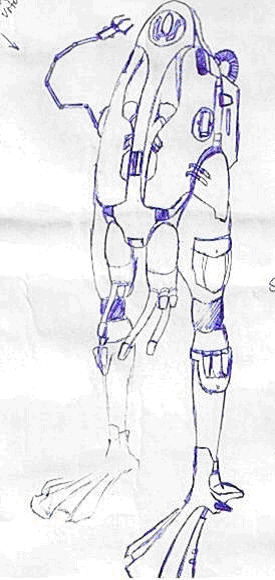
\includegraphics[width=0.25\textwidth]{images/Shmrn-pilot1.png}
}
    \caption{Shmrn Pilot(2)}
    \label{fig:Shmrn-pilot1}
\end{center}
\end{figure}
\begin{figure}
\begin{center}
\makebox[\textwidth][c]{
    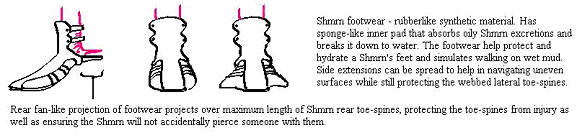
\includegraphics[width=\textwidth]{images/Shmrn-footwear.png}
}
    \caption{Shmrn footwear}
    \label{fig:Shmrn-footwear}
\end{center}
\end{figure}
\begin{figure}
\begin{center}
\makebox[\textwidth][c]{
    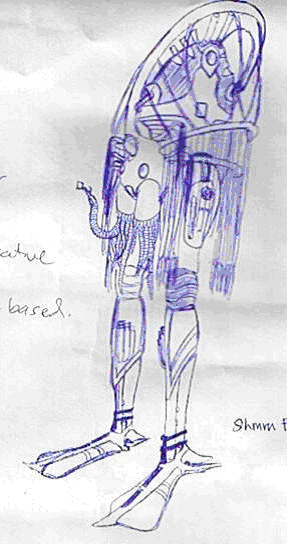
\includegraphics[width=0.5\textwidth]{images/Shmrn-formalwear.png}
}
    \caption{Shmrn formalwear}
    \label{fig:Shmrn-formalwear}
\end{center}
\end{figure}
\begin{figure}
\begin{center}
\makebox[\textwidth][c]{
    
\includegraphics[width=2in]{images/Shmrn-logo.png}
}
    \caption{Shmrn logo}
    \label{fig:Shmrn-logo}
\end{center}
\end{figure}
\begin{figure}
\begin{center}
\makebox[\textwidth][c]{
    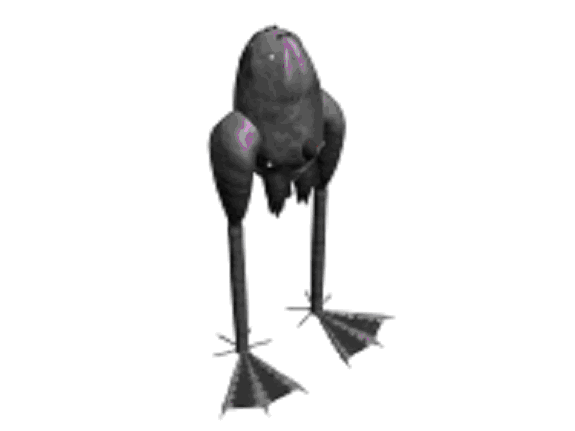
\includegraphics[width=\textwidth]{images/Shmrn-render.png}
}
    \caption{Shmrn - rendered}
    \label{fig:Shmrn-render}
\end{center}
\end{figure}

\subsection{Religion}
The Shmrn have a spiritual existence quite different from their
brothers the Dgn, with communal meetings contemplating the nature of
suffering over one's lifetimes dominating the organized religious
landscape. Shmrn culture and universe view centers on the principles
that life is unfair and painful, but a necessary stage to receive the
reward of eternal painlessness that awaits those who have, over
several lifetimes, overcome their desires to avoid the unpleasantness
of life.

\subsection{Miscellaneous}
Base 7. Nothing special. 

\section{Super Cetaceans (SuCets)}

Super Cetaceans (SuCets) are the result of what some consider the
first truly profound endeavours of Humanity in combining the fields of
genetics and cybernetics. While there are still SuCets around, they
are generally considered a "failed" experiment, never thinking in a
sufficiently compatible manner to become either useful tools or
partners, and requiring cybernetic additions that were too costly,
post nano-plague, for novelty value. Small communities of SuCets exist
on some of the more affluent and metropolitan oceanic worlds, and
their largest community, though quite small, remains on Earth.

\subsection{Physical characteristics}
The bulk of their genetic code derived from a potpourri of whales and
porpoises, they are oxygen breathing swimmers of immediately
recognizeable cetacean form, overcoming their lack of manipulator
limbs via integrated mechanical prosthesis.

\subsection{Habitat}
The shallower seas of the continental shelves and the vast waters of
oceans and oceanic worlds with oxygen-nitrogen atmospheres.

\section{Super Simians (SuSims)}

Super Simians (SuSims) and SuSim Cyborgs have been one of the more
stunting trends for "true" AIs, arising from the advances in the
fields of genetics and integrated cybernetics. For physically
manifested tasks considered too menial, too dangerous, or too
monotonous for Humans, the SuSims and SuSimCys proved cheaper, more
reliable, and, through advancements in genetics, easier to dominate
than AI alternatives.

As a client race they are quite prevalent in High-Born space as
servants. In other societies, however, the use of SuSims is seen as
inhumane or otherwise frowned upon.

\subsection{Physical characteristics}

The SuSims were constructed from augmented blends of Terran primates,
and many discernable features of their Chimpanzee and Bonobo ancestors
are immediately recognizeable. They remain hairy, not for practical
purposes, as much as to help convince their masters that the lines
between pet, tool, and slave have not been crossed in an era when some
"Humans" may be further distant genetically than the SuSims are from
Homo Sapiens Sapiens.

\subsection{Habitat}
They are capable of breathing an oxygen-nitrogen atmosphere. 

\section{Those who have only names (TWHON)}

What little is described of this group is gleaned from writings left
behind by the Ancients. While most descriptions are quite vague, it is
clear that TWHON, if the Ancients are a reliable source, were at least
as advanced as the Ancients, and much older.

\section{Uln}

FIXME 

\subsection{Physical characteristics}
 
8 limbs, 4 legs, 4 arms. Each arm end in a "hand" with 4 "fingers" one
of which is opposable. The four legs terminate in fleshy-padded feet,
each of which ends in sets of broad, thick, fore and back claws
capable of allowing "tree"-climbing. All four legs are visible in the
rear picture (this specimin has somewhat skinny front legs). The two
arm pairs are socketed between the two leg pairs, one pair of arms
reaching over the head, the other coming up from under. The head is
large and block-like, situated on a short, muscular stalk of a neck
protruding from the main torso. The main torso features twin rows of
breathing holes, visible on the back/underside.

There are 3 moving parts in the Uln jaw, a lower jaw, and two side
portions, all of which are normally involved in eating. There is a
single visual input band that stretches across the front and onto the
sides of the Uln head, forming a cover for their complicated compound
eye. Uln vision is actually remarkably good, and they can see from the
infrared/near-microwave into soft UV (hence, some interesting trends
in Uln clothing materials).

Figure~\ref{fig:Uln-bodyplan} sketches the basic shapes described above.

\begin{figure}
\begin{center}
\makebox[\textwidth][c]{
    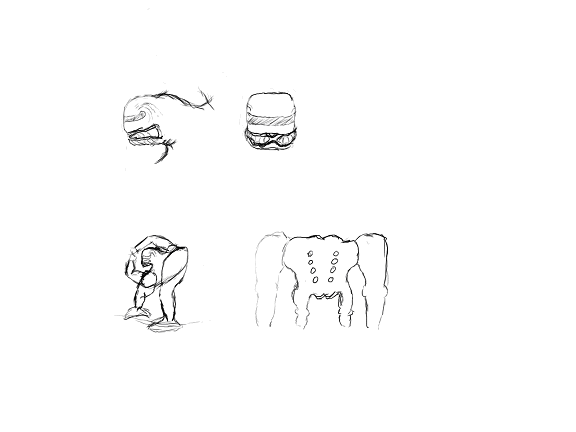
\includegraphics[width=\textwidth]{images/Uln-bodyplan.png}
}
    \caption{Partial sketches of Uln body plan, details of head.}
    \label{fig:Uln-bodyplan}
\end{center}
\end{figure}


\subsubsection{Digestion}

The Uln don't do well with carbonated beverages. At all. Their
digestive tract isn't suited to things that expand that rapidly upon
consumption, and they will make a horrid, stinky mess of things when
they exhibit that gem of convergent evolution (traditionally for toxin
removal) of spewing their food back out.

\subsection{Habitat}
FIXME 

Oxygen-Nitrogen.

       (Shmrn logo)


\subsection{Culture}
The Uln culture sprang up among the remains of a sprawling set of
Ancient structures and advanced in technology faster than their
biology or social structures could adapt, leading one noted human
researcher to note upon seeing them, "It was as if I had suddenly come
across a spacecraft piloted by Homo Erectus -- if they hadn't been so
ill prepared for the gifts they unintentionally received, they would
have conquered the entire arm." Fortunately for the aspirations of
dominance held by other species, the Uln were decidedly
unprepared. Indeed, they spent so much time blowing each other up with
weapons they didn't entirely control that it is a wonder that either
they or the ruins on their planet still survive.
\begin{itemize}
\item History

Uln development is somewhat difficult to follow, as they are not
actually "native" to their homeworld. Indeed, very little of the plant
and animal life on the entire planet appears to have been of native
origin, present for only millions of years. In particular, the species
on the planet appear to have come from many different origins, as is
sensible given the broad range over which Ancient sites have been
discovered in other star systems. The Uln are not generally very
talkative about their origins, especially as it is the common
agreement among the other sapients that they're the descendents of
whatever the Ancients were using for lab rats/monkeys. It is therefore
still a matter of some debate as to which features of the Uln are
naturally occurring, which were engineered, and what reasons there
were for such choices.

\item Clothing

The most commonly worn Uln garments range from "open-toed(clawed)"
short-boots, some utility pouches with straps around the upper arms
resting on the neck, and a helmet-scarf (draping down to cover more
sensitive regions between the underside of the neck and the lower
arms) which would be common casual-wear for the common peon, to the
foul-weather knee-length boots and helmet-poncho and the bizzare
extravagances of the aristocratic class, with gaudy creations not
unlike wearing an array of very fine wire-meshes and doilies, that
require servants to dress them. The back/underside is not normally
overly covered, though something may drape loosely behind the top arms
- to do otherwise would interfere with their breathing.
\end{itemize}
\subsection{Religion}
Growing up amidst the ruins of an exceptionally powerful and ancient
culture on a planet where life was artificially introduced gave the
Uln the idea that they were the children of failed gods. Convincing
them that they are much more likely the descendants of
lab-monkey-analogs from a long destroyed outpost hasn't gotten very
far. What passes for organization in Uln religion involves seasonal
festivals that mostly serve to reinforce the doctrinal line that being
born Uln is a wonderful thing, relative standard of living to the
other species be damned.

\subsection{Miscellaneous}
Base 4. Nothing special. 


\clearpage
\stepcounter{appendixcounter}
\refstepcounter{chapter}
\section*{Appendix \Alph{appendixcounter}: NAME OF APPENDIX}
\addcontentsline{toc}{chapter}{Appendix \Alph{appendixcounter}: NAME OF APPENDIX}
FACTIONS of the UTCS Time Period


FIXME

§	Confed IntelSec 
o	Confederation Navy 
o	Exploratory Service 
o	Concerned Confederation Citizens Against the War 
o	Confed Pleasure Planet Travel Consortium (CPPTC) 

\section{Aeran Ascendancy}

The Aeran Ascendency governs the Aerans and Bzbr. The Aeran Ascendancy
is, in practice, a body wholly controlled by entirely Aeran will of
the Aeran Oligarchy. All distinct Aeran subgroups, such as the Aeran
Merchant Marines are subject to the edicts of the Aeran Oligarchy.

\subsection{Aera}
Faction data 
Aera 
Species 	Aera 
Homeworld (Origin) 	Aeneth 
Capital 	Aeneth 


\subsubsection{A Brief History of the Aera}

The Aera homeworld was home to extremely competitive ecosystems. It
was not a supportive environment. If one considers Earth the "mother"
of the human race, then, in comparison, Aeneth was an abusive
parent. The Aera evolved in an environment where a slew of things
really did want to kill/eat/infest them. Beginning with the early
harnessing of fire, and ending with industrial might, the Aera
remedied this problem by destroying the vast jungles that bore
them. However, their outlook on the universe was fundamentally shaped
by their beginnings in a direction that humans would consider
paranoid, or at least profoundly pessimistic and somewhat untrusting,
though the Area merely see it as prudent recognition of how the
universe works.

This outlook was greatly reinforced by the Aera experience with the
nano-plague. The precocious Aera, unlike humans or Rlaan, developed
jump-based FTL before having otherwise left their solar system. The
resultant reactivation of the nano-plague and the devastation it
wrought on their population, served to gel their concept of an
inherently antagonistic universe. Aeran society greatly increased its
militarization, heretofore on the wane since global unification, so as
to better prepare for potential conflicts in what, evidenced by the
nano-plague, they presumed was an inhabited galaxy.

The Aera are the youngest of the three currently dominant space-faring
major groups, but are also the most expansionist, fastest breeding,
shortest lived, and devote the highest fraction of their economy to
military and military related R\&D spending. They are not evil, they
are not delusional, they are not irrational, but they have some
fundamentally different assumptions they are working from that make
them somewhat difficult to get along with. Finding out that their
section of the jump network had them pinned by the Humans and Rlaan,
they first attempted to negotiate passage, and were rebuffed. They
then attempted to sneak a colony convoy through Rlaan space, but this
turned into an utter debacle after Aeran escorts killed Rlaan
Civilians, sparking a war lasting several years, that churned the
Rlaan-Aeran border into an abattoir. Although formal peace has never
been brokered between the two, a cease-fire has been in effect for
several years. The Aera have now turned their sights toward Human
space, invading Forsaken territory, hoping to push through toward the
less defended Forsaken/Confederation border crossings, carve a
corridor through to the other side of humans space, and keep it open
long enough so that they can send enough colonization fleets through
to the other side to make the venture worthwhile.

\subsubsection{Development}
Compared to contemporary 33rd century humans, the Aera are comparable
or somewhat more advanced in some of the physical sciences and their
applications, notably so with respect weaponizations of certain
technologies. They are noticeably behind in life sciences and AI.

Having been wandering the jump network for the least amount of time
(among the Rlaan/Humans/Aera), the Aera, though occupying the same
order of magnitude of systems as the Humans or the Rlaan
(Rlaan/Lmpl/Nuhln/Saahasayaay have most, followed by
Humans/Klk'k/Dgn/Purth/Mishtali, followed by Aera/Bzbr, then the much
smaller Uln, Shmrn) have not occupied many of them for nearly as
long. The Aera expanded in territory faster than that territory could
be developed up until running into the Uln. After one last push then
brought them to the Human and Rlaan borders as well, the Aera have
been racing to build up their newly settled colonies nearer the
borders, but the bulk of their industrial potential remains
concentrated in systems closer to their homeworld than to alien
space. This difference was especially clear during the Rlaan-Aera
conflict, wherein many newly settled Aeran colonies along the border
fell to the Rlaan assault, but the same Rlaan fleets were badly
bloodied when they tried to push into Aeran systems with more matured
defenses. Due to the war, Aeran military spending and infrastructure
development has been extravagant in comparison to human budgets, but
the Aera also had to cope with sizeable losses in personnel and
materiel.

While there are key differences between the level of population and
industrial development between the core colonies and the newer
colonies, due to the very strong central organizing forces in Aeran
governance and economy, this is not a deep political divide, nor an
economic one - it is merely a matter of the more fringe planets
growing as fast as they can into states undifferentiable from the more
core worlds. This centralization should not be taken as evidence that
Aerans are a selfless society of collectivists. Rather, the Aera have
a strong natural ability and desire to sublimate personal interests to
higher authority, a trait left over from their more pack-like
origins. Success, however, is still judged at individual granularity,
and Aera are entirely opportunistic about personal advancement when
the opportunity either does not come at the expense of the dictates of
higher authority, or places them into a position of higher authority.

\subsubsection{Culture}
The Aera are a bit culturally dour, although they do engage in
organizational events, such as rallies, sporting contests, and
Military parades. Entertainment pursuits, such as music, for personal
pleasure are not a significant thread in Aeran culture. Such pursuits
are seen as necessary avenues of release, but to devote oneself to
pursuing purely entertainment oriented activities merely because they
are pleasant is seen as wasteful, wantonly hedonistic, and a reckless
abandonment of one's duties. Entertainment with physical components,
such as sporting competitions, are viewed in a more favorable light.

In Aeran culture, mortality is to be pondered and meditated upon in
its inevitability. It is worth noting that it is not so much those
that came before them that the Aera cherish as the accomplishments of
those who came before them. The Aera perspective is that it is only
though accomplishment on behalf of the Aera that the Aera can
continue, and the dead, thereby, can continue to live in the memories
of the Aera.

\subsubsection{Organization}
Aera culture is highly organized and decidedly hierarchical, but in
the form of a meritocracy rather than an aristocracy. While what has
constituted merit has morphed over the millennia since the first Aera
tribes selected work crews to cut back the encroachments of the jungle
upon their early settlements, given the relative position of the
pre-technological Aera in their local food chain, there has long been
a favoring of cleverness and determination over raw strength. The
current social and vocational position of any Aera is immediately
indicated by the color and pattern of an individual's coverall. The
Aera are ruled by a subset of the highest caste, with membership in
the oligarchy changing whenever either an individual steps down, or a
third of the other members call for a member's replacement. New
members must be confirmed by two thirds of the current oligarchy. It
is much more common for members to voluntarily remove themselves from
power, believing themselves more useful elsewhere in society, than to
be cast out. An average stay in the oligarchy lasts a few Aera years.

Need to more usefully carve up faction vs. species information. Will
do so later.FIXME

\subsection{Aeran Merchant Marine}

Faction data 
Merchant Marines 
Species 	Aera 
Homeworld (Origin) 	Aeneth 
Capital 	Aeneth 

The Aera don't really have a civilian sector. All Aera resources are
controlled by the state, and ruled over by the Oligarchy. The Aera do,
however differentiate between combatant and non-combatant forces, and
the Merchant Marine, while armed, are designed to transport goods
through dangerous space rather than conquer said space. (It may be
duly noted that the Aera are predisposed to consider all space to be
dangerous).

\subsection{Bzbr}

Faction data 
Bzbr 
Species 	Bzbr 
Homeworld (Origin) 	Fixme? 
Capital 	Fixme? 
	
The Bzbr are a client race uplifted by the Aera. They are reasonable
laborers, but poor conversationalists, in part due to their lack of
vocal cords.  The Aera uplifted the Bzbr out of pity for the Bzbr due
to similarities the Bzbr homeworld had with the Aera homeworld.

The Bzbr engage in significant hero worship of the Aera, although
indications are that the Aera are not appreciative of this
tendency. The Bzbr are wholly integrated into the Aeran Ascendency,
and given extremely little self-control as a group. Aeran officials
permeate their entire governmental structure, itself in parts borrowed
from and imposed by the Aerans upon the existing stone-age Bzbr. The
Bzbr, however, remain near universally accepting of their Aeran
overlords due to a combination of religious reverence and vast
improvements in their standards of living. Experiences during the
Rlaan/Aera conflict found Bzbr to be even less accepting than Aerans
of non-Aeran governance. Their fanatical level of religious devotion
to the Aera found them to be prime subjects for guerilla actions
involving the likely demise of the participants.


\section{Confederation of Inhabited Worlds}

Faction data 
Confed 
Species 	Humans, Klk'k, Purth, Dgn and Mishtali 
Homeworld (Origin) 	Various 
Capital 	Mars 

The Confederation of Inhabited Worlds (Confed) is made up of
partially-autonomous member states, and was created with a primary
purpose being to arbitrate disputes between them in a more structured
and less violent way than the Andolian-Lightbearer dispute was
handled. In addition to this, with the Klk'k representing a reasonably
advanced alien species and the Andolian-Lightbearer war pushing home
notions of the potential for interstellar war, a re-evaluation of the
need for maintaining a unified defensive force was seen to be in
order.

Each constituent state is allowed to maintain its own military forces,
but it must submit some portion of its resources to maintaining the
Confederation fleet, which is distinct from any state's military.

The confederation's rights over its constituent states are those and
only those so ceded by the constituent states in the confederation
constitution. Admittedly, exactly what rights were ceded is always a
debatable issue. Likewise, the confederation's unicameral legislature
has oft attempted to pass dubiously constitutional edicts. However,
the constitutionality of the Homeland Security Forces is actually
unimpeachable, as they were specifically called for in the
constitution to bypass the previously tangled web of extradition
policies between the constituent states and to force some measure of
legal compatibility between said states such that outright and overt
support for groups violently antagonistic to other member states would
not be tolerated. While none of the member states is particularly
ecstatic about the confederation's nature and its imposition on their
internal affairs, all are, at least publicly, thankful for the unified
front that allows humanity to operate alongside alien entities much
larger than any single member state.

The civilian center of the confederation as well as the fleet
headquarters is located on Mars since the Sol location is symbolic of
humanity's common roots. Earth came with too much political baggage,
and so Mars was chosen to be the center of the confederation. A
hierarchy of civilian and military installations then extends out from
Mars to the furthest reaches of confederation space. While sufficient
function is distributed redundantly to prevent a catastrophic
beheading, only the confed installations on Mars can be said to have
been designed with splendor in mind, and thus hold no rivals among the
other installations.




\subsection{Andolian Protectorate}
\index{Andolian!Andolian Protectorate}

Faction data 
Andolian Protectorate 
Species 	Human, Klk'k and Purth 
Homeworld (Origin) 	Various 
Capital 	Kubernan 

The Andolian Protectorate refers specifically to a government. 

\subsubsection{Members}

All Andolians are members of the Andolian Protectorate, not all
members of the Andolian Protectorate are Andolians. In particular,
there are Klk'k, Purth, and non-Andolian human citizens of the
Protectorate (the non-Andolian humans mostly being non-integrationist
members of annexed entities or yet to be integrated immigrants to the
Protectorate from other polities). Andolians, being the dominant
faction within the Protectorate, are good indicators of how the
Protectorate will act.

\subsubsection{History}

The Andolian Protectorate was created by the Andolians as the
political entity controlling both Andolian and Klk'k interests. During
the formation of the Confederation, there was some consolidation of
minor factions, bringing an influx of non-Andolian humans into the
Protectorate (an extremely small minority of the human population born
into the Protectorate remains non-Andolian - less than 1\% of the total
human population). Many Klk'k are more accurately considered Andolian
at present (in ideological adherence), but the integrated Klk'k are a
distinct minority of the total Klk'k population, which is
ideologically more diverse.


\subsubsection{Andolians}

Faction data 
Andolians 
Species 	Human, primarily of the Pluralis variant. 
Homeworld (Origin) 	Earth 
Capital 	Kubernan 

Andolians are a human faction primarily consisting of the Pluralis
variant well developed in both information and physical resources. All
Andolians are members of the Andolian Protectorate but maintain a
subordinate government concerned with Andolian affairs.

Many of the major Human governments could be considered "ideocracies"
wherein a supermajority, often a near totality, of the population
governed by an entity are adherents of a given ideological
perspective. The Andolians were such a group, with a clear
correspondance between the Andolians (the adherents) and the Andolians
(the political entity controlled by the adherents) until the Andolians
came to have a more diverse political landscape when they became
Protectors of the Klk'k population, and later, the Purth. Many Klk'k
have since become integrated with the Andolian mainstream, but the
Protectorate remains more ideologically diverse than the Andolians
proper.

Needs more FIXME 

\subsubsection{Klk'k}

Faction data 
Klk'k 
Species 	Klk'k 
Homeworld (Origin) 	Ktah 
Capital 	Ktah 
Needs a better desc FIXME 

The Klk'k are a client race of the Andolians, but enjoy exceptional
freedom within this position. Indeed, while fiercely loyal to their
Andolian benefactors, there exist a non-trivial number of
independently operated Klk'k vessels. The Klk'k are perhaps best known
for their odd brand of twisted humor.

\subsubsection{Purth}
\index{Andolian@Purth}
\index{Purth@\textit{Purth}}

Faction data 
Purth 
Species 	Purth 
Homeworld (Origin) 	fixme 
Capital 	fixme 

The Purth are politically subserviant members of the Andolian
Protectorate, heavily reliant in most facets of their existence upon
the assistance of the Klk'k and Human members of the Protectorate. The
Purth do not operate independently, instead being heavily integrated
into the Protectorate military forces, as might be expected given
their origins as a cybernetics research project.  FIXME

\subsubsection{Spaceborn}

Faction data 
Spaceborn 
Species 	Spaceborn 
Homeworld (Origin) 	Cradle
Capital 	Kubernan 

Those Spaceborn who chose to remain as such rather than attempt to
reintegrate into more mainline human gene-pools live almost
exclusively under the auspices of their liberators, the Andolian
Protectorate. The Spaceborn make up a miniscule fraction of the total
Protectorate population, but are heavily involved in many of the
Protectorate's free-space construction and maintenance projects.


\subsection{Highborn}

Faction data 
Highborn 
Species 	Humans 
Homeworld (Origin) 	Earth 
Capital 	Fixme? 

The Highborn are a human faction better known for its disregard for
life than its art or achievement.

They are one of the oldest colonial groups and had significant
resources on Earth, lending them the cream of the initial colony
locations. They were the main defenders of the 1st Confed Party
Reform, which had forbidden the ISO.  Primary manufacturers of dueling
weaponry.  Motto: "There is no substitute for a superior human being."

\subsection{Homeland Security}

Faction data 
Homeland Security 
Species 	Human 
Homeworld (Origin) 	Earth 
Capital 	Mars 

The Homeland Security forces are primarily composed of Purists but
contain members from most human groups. The Homeland Security forces
exist for internal policing and control, especially in cases crossing
between the jurisdictional boundaries of member states of the
Confederation, as they are an arm of the Confederation rather an
amalgamation of forces from member states. While distinctly limited by
both practical and political concerns in how much pressure they can
bring to bear if a member state actively obstructs the pursuit of
their duties, they counterbalance by being more authoritarian then
generally deemed necessary within what is clearly their own
domain. This is known to be especially true of the IntelSec wing of
the Homeland Security Forces.

\subsection{Hunters}

Faction data 
Hunter 
Species 	Humans 
Homeworld (Origin) 	Earth 
Capital 	Non-governmental group. 

Arising in the profit opportunities of the lawlessness of the Diamond
Dust period, various mercenary groups underwent iterations of
consolidation due to expanding polities, increasing regulation, and a
decline in per-capita bounty-hunting opportunities. While still
comprised of numerous independent groups of guns-for-hire, the
Hunter's guild provides a unified interface for those seeking their
still-needed services and a well-financed legal wing to make sure that
bounty hunting remains as legal as it is profitable.

\subsection{League of Independent Human Worlds}

Faction data 
LIHW 
Species 	Human 
Homeworld (Origin) 	Earth 
Capital 	FIXME

Scattered across the frontiers of known space are many worlds housing
minor subsets of humanity which hold no place among the larger
meme-group entities.

Humanity has, throughout the past, been an oft balkanized lot. While
the bulk of human power and population has, for various reasons,
aligned itself with one of the major or minor meme-groups there are
many colonies, that, for reasons of either intense pluralism or
adherence to a tertiary meme-group have remained independent (examples
of such being the inhabitants of Vegan-ville, or the citizens of the
"Brotherhood of Militant Agnostics" (motto: "I don't know, and neither
do you!") ).

But in the wake of the Mankind's first notable interstellar fraternal
conflict--the demolishing of the Lightbearers by the Andolians--and
the efforts which followed in the founding of the Confed, whose
membership consists of the major meme-groups, the bulk of the lesser
subsets realized that--while they may not get along all that well with
each other--if they did not in some way present a united front of
resistance, they would likely be consumed by the major meme-groups. As
such, they joined the Confed united as the League of Independent Human
Worlds (LIHW), and, counter-intuitively, gained, through their
co-operation, a guarantee of protection of their individual and often
separatist modes of life.

Those that did not band together or exit en mass to Forsaken space,
are now only records in history books, having been overrun, subverted,
co-opted, or in other ways gobbled up by the major meme-groups.

\subsection{Mechanists}

Faction data 
Mechanist 
Species 	Mechanist 
Homeworld (Origin) 	Earth 
Capital 	Plato
FIXME Stub entry - taken from dynamic\_news\_content.py 
·	Full faction name: Mandate for Corporeal Perfection via the Abandonment of Flesh 
·	Government name: Concordance of Enlightened Ones 

\subsection{Merchant's Guild}

Faction data 
Interstellar Shipping and Mercantile Guild 
Species 	Humans 
Homeworld (Origin) 	Earth 
Capital 	Bantam 

A latecomer to the great sowing of Earth's seeds, a too-small planet,
previously passed over, became the new home for a group of colonists
united more by a desire to leave behind their varied existences in Sol
than by any common ethos. The colonists struck out from their
settlements in the deep canyons and valleys where the air was thicker,
clearing out the simple layers of native life, ever so slowly etching
humanity's presence indelibly into the planet's crust. However, the
future of their efforts did not lie on the surface of a world, but in
the cold of space surrounding it.

No too-small world can hope to passively hold on to the sort of
atmosphere that gives rise to sunny, green meadows alight with
frolicking schoolchildren. The release from the domes, from the deep
places, would be a Herculean task, but the insights bestowed by modern
science had given mere mortal men more abilities than the authors of
the ancient demigod had foreseen. In a common goal, the residents of
Bantam found new unity and identity. They labored together tirelessly
to construct the centerpiece of their terraforming effort: a colossal
station that would serve as both the shipyard producing and
maintaining the resource gathering fleet and the processing center
that would amalgamate the offerings of the entire system into
sustenance for Bantam's development.

It would likely have worked. 

The nano-plague struck without warning, long before the first human
FTL ship would visit the system. Only the near-paranoid levels of
over-engineering with which Rainbow station had been constructed saved
it from the fate of many of Bantam's residents, too reliant on cheap
and plentiful nanites. It was far too early in the terraforming effort
to live in the open, and suddenly overstrained environmental systems
caused entire cities to suffocate. Bantam was devastated, losing all
vibrancy and vitality in a matter of weeks. What before had been a
growing planet-wide civilization was now a collection of frightened
outposts of inhabitation. Thus were Rainbow station and its infant
fleet of resource gatherers nearly orphaned, the mother planet an
invalid. With the station barely able to sustain itself, the
stationers were left with the unenviable role of deciding whom amongst
Bantam's survivors they could afford to save.

As the Diamond Dust Age progressed, and Bantam continued to wither
away to a pale shadow of its brief heyday, Rainbow station endured,
growing throughout the period of isolation, if at a glacial
pace. Warning messages, lazily arriving at the speed of light from
their neighbors, came in one after the other, followed sometimes by
descriptions of chaos, and sometimes by silence. There was no official
expectation of assistance, but humans are renowned for their
counter-empirical optimism.

Thus, it was with great surprise and anticipation that the arrival of
the first FTL ship was greeted, and numbing disappointment the feeling
that swept the stationers when they learned that it was not a portend
of any mission of mercy. All, however, did not look grim. The visitors
were High-Born explorers, but from a family of lower standing. The
Marcos family realized that they had much to gain from control of
Rainbow station once it began producing jump capable vessels. With FTL
technology and the silent threat of a second abandonment for leverage,
the Marcos family gained a large stake in Rainbow station.

Luck had indeed changed for the better for the people of Bantam and
Rainbow. Not only were much needed resources flowing in from High-Born
space, payments for an ever increasing list of ship construction
orders, but Rainbow soon proved itself to occupy a prime location in
the jump network, a hub on what would remain for many decades the only
practical routes connecting several populous systems to each other -
including Sol.

Some colonies had fallen far and some had not had far to fall. The
lone merchant was a valuable target in a starved land. Neither were
the financial benefits of collusion upon profit margins lost upon the
increasing number of traders operating out of or, less commonly at the
time, passing through Rainbow. The first of the great mercantile
cartels was formed, again under the leadership of the Marcos clan, a
silent, nameless cartel that worked to establish a near monopoly on
interstellar trade in much of human space during the Reconstruction
period. Coercion, cooption, and even the occasional assassination were
all valid tools to grow the blossoming financial empire centered on
Rainbow and the slowly awakening Bantam. The Rainbow station cartel
was one of a few groups to capitalize upon the realization that, in
the absence of any overarching authorities, whomsoever dominated the
trade lanes now could well be able to do so for centuries to come,
barring fantastic advances in interstellar travel.

Generations passed. Competitors fell as they came, though some
struggled valiantly, and only the governments of the larger
meme-groups were sufficiently imposing to hold their own at the
bargaining tables. Shares of control of Rainbow station changed hands,
and it became wholly an instrument of the cartel, although Bantam and
Stationer descendants still held a plurality of control of the cartel,
a sizeable majority if one included the increasingly integrated Marcos
clan. The name of the station changed then as well, and the cartel
gained a name, rechristened Cherryh station and the Cherryh Mercantile
Trust (CMT), respectively.

Though flagrantly in bed with High-Born interests, the CMT maintained
a resolute official neutrality, even going so far as to make a point
of hiring other parties for anti-piracy protection rather than
building their own combat fleets. While many at the time took this to
be a purely political maneuver, those more informed knew that it was
actually a necessity. Cherryh station had been a vital trump card for
the CMT in the early portions of the Reconstruction period, but
mankind had recovered somewhat, and was once more advancing, and the
age of the station was beginning to show. Bulk freighters are in many
ways much easier to build than the tiny craft that protect them and
avoid obsolescence much longer, and Cherryh station was only up to the
task of constructing the first, and not the latter.

More modern shipyards, though not on the scale of the CMT's aging
beauty, were being constructed all over, and the competitive advantage
the CMT had enjoyed due to their production capacity was waning. There
was, however, little feared by the CMT at this point, as there was no
longer any competition of note to gain upon them. All other transport
of goods was in-system, governmental, or doomed to obscurity or
absorption. The CMT used this time to increase its wealth, strengthen
and modernize its infrastructure, and deepen its influence on various
governments. The resettlement of Bantam was in full swing.

The CMT's opportunity to rest did not last as long as they would have
preferred. The development of the SPEC drive dramatically changed the
landscape of trade routes, altered latencies, and made runs by smaller
vessels much more practical. Rapidly expanding borders made for new
regions for local competitors to exploit more rapidly than the CMT
might be able to react. However, like the age itself, the CMT had
matured. There would be no massive wave of assassinations or stream of
engineered third-party blockades. Rather, there would be the ultimate
buy-out - the largest recruitment effort ever mounted, a clarion call
summoning all traders to a common banner with the offer of common
profits. What could have been the death knell for the CMT merely
announced the birth of the Interstellar Shipping and Mercantile Guild,
which if it still had the CMT at its core, was, by the nature of its
creation, intended to be a beast with a very different public face.

The emergence of the Confederation only served to strengthen the
position of the Guild, being included in the Confederation Senate's
Committees despite technically only owning a single star system (the
plethora of commerce stations and trading outposts in the star systems
of other powers not counting as seats of population) - an important
technicality, as it would otherwise be difficult to pretend they were
a governmental entity in the same sense as the other Senate
members. The newly formed Confederation Navy and Homeland Security
forces served to decrease piracy along standard trade routes, even if
the decline of several independent powers in the face of enforcing new
Confederation regulations gave rise to a whole new breed of
paramilitary forces. While in matters internal to the Confederation
the Guild was still maintaining an increasingly less fictitious
neutrality on matters not of self-interest, there was no love lost
between the Forsaken and the Guild, the much lower profit margins
available on return trips never having enticed much Guild investment,
and Guild price fixing long having raised the ire of the
Forsaken. Guild presence in Forsaken space is thus limited to border
stations, much like the trade relations with the Uln and Rlaan.

Contact with alien trading partners was a great boon to the Guild, as
Guild political clout ensured that all major alien traffic would pass
through Guild trading stations, that Guild shipping would be awarded
nearly all lucrative inter-government contracts calling for human
merchants, and so forth. Moreover, no independent trader could so
easily call upon the shared resources of the Guild in obtaining
appropriate permissions from the Uln and Rlaan governments to conduct
business within their borders, or the expertise of a cultural
specialist in determining the likely intentions of an alien customer.

Though the upper echelons of the Guild are still plentifully stocked
with CMT personnel, the Guild favored success over nepotism, and many
rose through the ranks to positions of power - unlike the larger
meme-groups, no grand conversion of belief system is required for
acceptance, merely the conviction that profit conquers all, and timely
payment of portions thereof. The lower tiers of the Guild are full of
all sort and manner of small time traders who were willing to trade a
fraction of their profits for protection, access, and
opportunity. Unlike the pre-SPEC period, the smaller independent
traders are not actively squashed, and those who achieve success are
always initially courted rather than destroyed outright, but this is
largely because any emerging independent group which appeared to offer
a real threat would be rapidly legislated out of existence by calling
in favors in the Confederation Senate. The current Guild is rivaled
only by the logistical corps of some major meme-groups that did not
desire to give up the independence of their internal supply chains,
but even these entities are dwarfish by comparison. Though still not a
military power, nor aspiring to become one, the Guild's numerous
shipyards, kept modernized under lucrative Confederation contracts now
churn out capital and sub-capital military vessels for the
Confederation Navy alongside their freight bearing kin. With the
renovation of Cherryh station over the last few decades further
boosting production, the Guild shipyards maintain a distinct lead, by
tonnage, as the largest suppliers of Confederation military vessels.

\subsection{Purist}

Faction data 
Purist 
Species 	Human 
Homeworld (Origin) 	Earth 
Capital 	Earth 

A surprisingly large memegroup, and the dominant one in Sol, the
Purists seek a humanity free of changes to the species. They do not
stand for non-therapudic genetic modification, nor for unnecessary
cybernetic implants. They are, however, not opposed to technology
which is not used to alter humans. Motto: In being what we are, become
all that we can be.






\subsection{Shapers}

Faction data 
Shaper 
Species 	Human 
Homeworld (Origin) 	Earth 
Capital 	Bifröst 

The Shaper government, such as one exists, was originally constructed
along 'libertarian' lines (albeit with some elements that would seem
deeply foreign or even perhaps contradictory to any person harking to
the same 'libertarian' title who is not also a devotee of the Shaper
ideology), and is a generally minimalist entity, delegating many of
the tasks performed by the other human governments to private
interests within the Shaper populace. Confoundingly, the Shaper views
on children are remarkably collectivist, and closely tied to the
particular Shaper notions of what constitutes an actual human
existence. Government social programs are unheard of for adults, but
heavily invested for children, and while there are a number of
government standards committees, they almost exclusively produce
guidelines, rather than regulations. Government interference into the
economy is utterly untolerated. Individual civil liberties are
fiercely protected, and one of the more significantly funded programs,
aside from defense spending, is the publicly funded "Authority
Surveillance Guardianship" or ASGuard, the funding for which and chief
administrators of being determined directly by the Shaper populace.

Shaper society is egalitarian in opportunity, but extremely
competitive and indifferent, when not outright unforgiving, of
failure, with notable emphasis being put into ensuring that the
failings of members of one generation are not allowed to be magnified
through their offspring. Notably, procreation in any form (be it
cloning, or gene-mixing, or more traditional conception) is not
considered a right within Shaper society. The furtherance of one's
genetic material is deemed a privilege of personal success. Attempting
to raise Shaper children without appropriate resources or accepted
competence in child-rearing is considered criminally abusive of the
children. Non-Shaper children have a decidedly different legal status,
are protected only in a sense of general 'human' liberties, and are
under no circumstances the recipients of collective support.

It should be noted that childhood is a rather abbreviated thing in
Shaper society, due to genetic engineering and common practices
greatly affecting both pre-natal and post-natal growth and
learning. Natural childbirth is seen as exceptionally eccentric within
Shaper society and is tolerated in much the same way that artists in
the 20th century who deigned to use their own bodily fluids in their
artwork were tolerated, but far from welcomed. Normal Shaper children
are born in child producing factories, more often than not, with the
exception of vanity children, being very carefully designed from mixes
of parental DNA with sequences from currently popular designs. The
gestation period in such factories tends to runs toward 14 months, a
length second only to Andolian full-growth gestation-immersion tanks -
unlike the other cultures using the tanks to replace normal childbirth
where the delay of from conception to birth is often seen as an
inconvenience to the prospective parents and time-to-delivery is
generally minimized, Shaper society considers the physically
ineffectual infancy of normal humanity far more inconvenient (and
repugnantly archaic - an evolutionary solution from before our own
evolution was ours to control) than the delay. Shaper children leave
the tanks already able to walk, run, and metabolize most foods - which
is important, as they have a voracious metabolism that will lead them
to grow to their adult mass within another 7 years. Brain development
in Shaper children is also accelerated. The mind is extremely plastic
for the first two years post-natal, and allows for socialization and
other acclimating patterns to form via processes still analogous to
those of a human child, if a somewhat precocious and extremely
intelligent one. The brain then rapidly proceeds to develop fully all
of its cognitive regions, at the expense of much of the childlike
plasticity for reorganization, and the Shaper child begins their
"adolescence", a state lasting from age two through seven, during
which they will leave the direct care of their parents, and begin to
compete against one another to be able to progress through an
assortment of privately run educational facilities (albeit the
students themselves are still collectively supported at this
point). The general educational period lasts an intense five years,
ending at the same time as Shaper children achieve physical and legal
adulthood and are no longer supported in any collective fashion. This
academic feat is made possible by the extremely low sleep needs of the
Shaper body, the lack of any need to exercise or endure sun exposure
in order to maintain health and muscle tone, and the
genetically-engineered capacity for extreme focus, easy memorization,
and ravenous intellect that every Shaper is possessed of.

For those not at the top of the competition, they remain free to
choose their path, but even the dullest Shaper is more than bright
enough, and by the turn of adulthood, sufficiently scrubbed of initial
ignorance, to understand with fair clarity where they are likeliest to
find others willing to choose them, and the importance of their own
below-the-billing role in Shaper society. The Shaper population is not
very densely arrayed on their planets, and the most menial tasks are
handled by Dgn, engineered lifeforms, and machines. While the Shapers
utilize AIs, the bulk of these AIs, for the past several hundred
years, have generally been of foreign construction, and the Shapers
are somewhat wary of the allegiances of the AIs in their employ - both
to other AI entities and to their constructors. A number of Shaper
specialists are therefore employed to monitor the AIs, and some Shaper
research has gone into developing minds better suited to such
tasks. Social unrest remains extremely low among the Shaper population
- Shaper society is not utopian, but it is without noticeable friction
- despite the intense competition and uneven distribution of
resources. This is largely due to the firmness of belief in the Shaper
ideology ingrained into the population - the underlying rightness of
the system of struggle is accepted, the rightness of the goals of the
society unquestioned, and those involved are possessed of minds
capable of understanding how they have come to occupy their place in
society, their role in that society and its continued existence, and,
just as importantly, how other individuals in Shaper society fit into
the greater picture. They operate with self-interest, but informed,
exquisitely reasoned, and long-termed self-interest that includes a
notion of Shaper society that has been made difficult to cast as
counter to personal interests.

For those who succeed, there is more than time for art - to practice
The Art is success. In the Shaper ethos, design is king, and flesh is
the favored palette. Thus, Shaper spacecraft, if not aesthetically
neglected as with the Mechanists, and, to an arguably lesser extent,
the Unadorned, are not anywhere near as profound as their work
groundside. While there is some artistry at work in their inanimate
constructions, working with metal and stone is as cold as either to
the Shaper mind: pale when compared to the calling to bend the path of
life to one's will, expressed for as long as the creations may
continue to survive their competitors and environs. Those tools, such
as spacecraft, of which great functionality is demanded, suffer
greatly in relative aesthetics to architectures that may be bent to
support the aesthetic demands of myriad Shaper minds, writ in living
spaces filled with living things, but only those living things chosen
to be there. While this leads to jaw-dropping wonderlands of living
material populating their art-oriented enclosures and an enjoyable
spread of magnificent creations adorning most living areas, the
exercise in control over what life lives where leaves Shaper planets
as devoid of real wilderness as an industrial farming world, if far
prettier for the same detriment. There is a sense that even a vast
uninhabited stretch on a Shaper world, possessed of some paradise-like
qualities in its safety and provision as it may be, is just a
carefully tended garden laying fallow for future inhabitants to
paint. There is chaos allowed to taint the waiting land. Nature is not
allowed to sully any canvas destined for Shaper hands.

The outside observer rarely tends to have their eyes drawn to the
Shaper underachievers, both because of the higher standards of living
(relative to Purist worlds, for instance), even on the low end, that
the Shaper economy has (made possible, in large part, by limiting the
population density on Shaper worlds), and the astounding beauty that
the high end of the Shaper culture produces. There is a Shaper saying
that, "It is no accident that the path to perfection travels through
beauty." The functional and aesthetic are merged whenever tenable in
Shaper society, and there is a significant place reserved for the
aesthetic, even absent, though rarely in lieu of, the functional. To
create more perfectly is the pervasive goal, and beauty is often
aligned with the perfect for anything that must be seen. It should be
noted that Shaper artists have produced works considered masterpieces
in a plethora of genres, as is not unexpected given a population
wherein even the dullest of healthy individuals would have been
considered quite mentally gifted in millennia past - however, within
Shaper society itself, only the construction of life-art is held in
meaningful esteem. Other venues for expression are welcomed, but
reserved for hobbyists and amateurs, not professionals. To construct
epic compositions in and of the human form is the highest art in
Shaper society. As full of science and practical consideration as
their genepool is, it is also their most holy of pieces of art, and
those who have risen to operate upon it their idols.

There are three common Shaper forms. In decreasing order of
population, these are females, males, neuters. A fourth form, the
'hulk', is only debatably a "Shaper form" and even more divergent from
the human strain than the Shapers themselves - however as they are
non-reproducing, few in number, have limited interaction with the rest
of Shaper society, and are distinct in construction based upon their
version and intended purpose, it is easier to consider them apart from
the Shaper populace and group them with other designer human life
forms, despite being of Shaper origin and mentality. The first
females, males, and neuters are of the same height, and all beautiful
by most standards, providing the lack of hair is not a deterrent to
such a judgment being rendered, nor the lack of nipples on Shaper
males and neuters found distrubing. Shapers are not muscle-bound, but
neither are they in any way waifish, with toned and sleek muscles
making their presence subtly known underneath taut skin - their
physique sometimes evokes images of acrobats, swimmers, and dancers,
depending upon which portions thereof were being used for the
metaphor. All Shapers are in prime physical condition both for
strength and endurance, although there exist plenty of custom bio-mods
who are stronger or have higher endurance. Shapers remain in prime
condition without need for exercise. Neuters carry both male and
female genetic code, but do not express either set of reproductive
organs or secondary sexual characteristics, earning them nicknames
associated with old plastic dolls. Instead of physical features to
distinguish Shapers from one another, with their near-singular skin
and eye color and lack of hair to style, Shapers tend to use clothing
and other symbiotic adornments when wishing to express their
individuality. Even then, a non-Shaper would find it extremely
difficult to identify which Shaper is which. Although much diverted
genetically from most humans, they are still capable of producing
fertile offspring with other human subspecies. Though a misnomer, as
many of the genes require either a Shaper female's womb or a
Shaper-compatible gestation tank to activate, "half-Shapers" arising
from Shaper males fertilizing non-Shaper females are not uncommon
among most human factions, as restrictions on Shaper procreation
privileges do not extend to the production of non-Shaper children
("half-Shapers" are not eligible to become Shaper citizens and are
subject to the same stringent residency requirements as any other
non-Shaper wishing to settle on a Shaper planet). Far more rare are
"incomplete-Shapers" - those born to a Shaper mother by a non-Shaper
father, or otherwise gestated in a Shaper compatible tank. As the
Shaper genes, when activated, tend to be dominant,
"incomplete-Shapers" tend to much more strongly express their Shaper
heritage, although they are still not legally considered
Shapers. Those with Shaper ancestors are commonly recognizable for
their generally gray to blue-black skin, often violet irises set in
gray eyes, and sparse body hair, although it is difficult, if not
sometimes nearly impossible, to distinguish between those with Shaper
ancestors and those who are the product or progeny of the custom
bio-modified.

Shaper clothing tends to fall into one of two very distinct
categories. Shapers have exceptionally minimal body modesty, and any
wearing of clothing whose primary purpose is to keep portions of the
body hidden from sight is done so on account of the modesty of
non-Shapers with whom they must interact - after all, the Shaper body
is a work of art and science they are proud to display. Shaper
work/functional clothes, therefore, act primarily to protect more
sensitive surfaces, to keep softer tissues in place during
motion/exertion, and to provide convenient places to store objects
being used. Such clothes are considered artful to the degree that they
do not interfere with the natural Shaper form and movement thereof. On
the other hand, as Shaper mastery both of their own body and their
environment is very advanced, with clothing for them somewhat
superfluous save for statement anyway in most climes and many
conditions, Shaper art-wear is something else entirely. High-end
Shaper art-wear often takes the form a living, generally translucent
expanse of vegetation designed at the protein and genome level by the
wearer - anything from a thin film, to a sheet-like wrap, to a
crawling expanse of vines, flowering if watered. Those less talented,
but financially equipped, will pay top credits to be similarly
designed for and decorated. Those in neither situation may opt to
obtain a license to perform minor customizations on existing designs,
or, for the even lower social rungs, to simply wear something mass
marketed - the Shaper equivalent of a cheap suit. Less common, but far
from rare, are non-vegetable incarnations of the above. Also common in
Shaper fashion are full-body markings and bioluminescent symbiotes
worn in lieu of jewelery. Full-body markings are normally applied by
developing pore patterns in body-sized engineered leaves that will
leave temporary colorations when wrapped around the body. Shaper
art-wear, though itself only exported as a luxury item, has become
very influential to Highborn fashion. Luxury items such as art-wear
and living rugs account for a noteworthy portion of Shaper exports, in
keeping with the unmatched tangible beauty of Shaper art. This
tangible and enduring nature, and it's profitable export, stands in
stark contrast to the only other major society with a comparable
number of artists, the Andolians, whose art the link-blind cannot even
sense, and whose works come and vanish on whim.

The Shapers are quietly contemptuous of most other meme-groups. They
find the Purists shameful, the Unadorned defective, the Highborn
arrogant and outmoded, the Merchants merely an unfortunate necessity,
and the Mechanists downright repulsive. Though they disagree
vehemently with the Andolians on a number of fundamental premises and
future directions, they respect them for their accomplishments. The
Shapers find the Rlaan interesting, the Uln pitiful, and the Aera
worthy, if unsympathetic, adversaries, if hopeless materialist
aesthetes incapable of appreciating life in any way valuable to the
Shapers.

The Shapers, with their superhuman aims, were a pre-Diaspora offshoot
of what later became the larger, supra-human aiming Lightbearer
meme-group. The two groups had wildly diverging goals and methodology,
despite both seeking a sort of embodied human perfection. Expedience,
however, makes strange bedfellows. Through location and shared
technological expertise, each group had something to offer the other,
even if each found the other ideologically perverse. Thus, what began
as a minor Shaper investment into a Lightbearer mission that would
bear closer to Shaper than Lightbearer space blossomed into a wary
partnership when the discovery of the ancestral Dgn made the Shaper
experience with non-human genetics immediately more valuable. However,
the partnership with the Lightbearers was not particularly long-lived,
as ideological differences made it exceptionally difficult for either
side to continue to operate in good faith absent obvious mutual
advantage, and by the time the aptly named Beckett's Murky Venture had
been exploited, there was little obvious advantage to continued
pretense of cooperation. Initial Shaper political, financial, and
resource support for the Lightbearers during the Fraternal War was
linked not to political or ideological support of the Lightbearers,
but a firm opposition to what they felt to be Andolian Imperialism and
the desecration of the natural sovereignty of the Lightbearers -
clearly, it didn't help that the Shapers thought the Andolians to be
even more ideologically disturbed than the Lightbearers; while the
Shapers thought the Lightbearers perversely misguided in their vision
of embodied human perfection, it was at least a goal that resonated
with their society, whereas the Andolian lust for abstract and
vaporous group progress that would somehow lead to a "bettering" of
mankind and thereby the individuals thereof struck the individualist
Shapers as a demented non-sequitur that was downright
unintelligible. The interjection of an expanding, and, if human,
foreign in an almost alien sense entity into a neighboring polity was
clearly cause for alarm, never mind the Klk'k - they, after all,
weren't human. That the Shapers cut off all support for the
Lightbearers after the revelation of the existence of the Spaceborn
indicates, importantly, that, at the time, they either thought us, or
themselves (depending upon one's perspective) to still be human, and
thus deserving of the fundamental human rights that run through the
core of their belief system. While some Lightbearers did flee to some
degree of protection within Shaper systems toward the end of the war,
it was that same sort of protection offered Nazi scientists captured
by the Russians after World War two - protection of ones life, but not
an opportunity to live, only an opportunity to be worked until
whatever useful knowledge you had could be extracted and you yourself
forgotten. Much has been rumored, but little ever confirmed about what
exactly occurred when the Simons later conducted raids into labs
believed to be housing unaccounted for Lightbearers in Shaper
space. It is well known that the Shapers were absolutely livid over
the Lightbearers' use of human slaves, and it is suspected that a far
darker hell awaited those who fled to Shaper space than they expected.

Notably, the Shapers never gave any indication that they were incensed
by the detailed descriptions of what the Lightbearers had subjected
the Shmrn to, and it is generally conjectured that they were privy to
that information long prior to its distribution by the
Andolians. Apparently, giving the Shmrn a strongly defined sense of
self, dignity, modesty, and a mind muddied by the introduction of
human derived genetic codes for brain development, all in the name of
allowing the Shmrn to truly appreciate and understand the physical and
emotional torture and suffering being inflicted upon them by the
Lightbearers in a way that the Lightbearers themselves could
understand, was not cause for outrage in the Shaper population because
the Shmrn weren't human. This lack of response, though attributed by
some as merely arising from their part in creating the Shmrn, led many
to believe that, if and when the Shapers considered themselves or the
rest of humanity to no longer be human, similar indifference could be
expected to follow were anything to come to affect the rest of
humanity differently than the Shapers. The topic of rights for
associated non-human species has continued to be a topic of contention
between Confederation factions, with the Andolians and the Shapers
tending to lead very different camps in such discussions. Likewise,
even on the topic of human rights, the different principles held by
the Andolians and Shapers has led to rather different stances being
taken on a number of policy decisions. On the topic of human slavery,
however, the two groups stand united, a unity that was formative in
the early Confederation.

Human slavery, as a viable economic pillar, died with the industrial
revolution. Human slavery, for personal pride, amusement, or
perversion, was reborn with mastery over the genome. No longer was it
necessary to steal away random human flotsam and unprotected child
assets, instilling fear and bringing hatred upon the slave trader -
instead, human flesh could be molded into whatever form the customer
desired, and raised from birth into servitude, birthed from a machine
without commentary on the subject. It became difficult in some places
to distinguish between slavery and child abuse. Such undertakings
remained quiet sorts of enterprises until after humanity had finally
ridden nano-technology and genetics to a post-sufficiency economy. In
the introverted, contented meme-group world of that past, the only
objection to someone outside one's meme-group raising slaves was one
of purely moral basis - it was simply unlikely to affect those outside
the participating meme-group. As SuSims, human-derived PAIs, and other
genetically engineered servant species became more increasingly
prevalent, it was increasingly difficult to gain a motivating
consensus on the issue when, despite many believing that human slavery
was over some line, agreement on where in the gray murk such a line
existed was not forthcoming.

It was not until the formation of the Confederation that such things
truly changed. All were free to not do business with polities allowing
behavior deemed "objectionable", but with the Confederation, a
sufficiently forceful hand could be put upon the hilt of a very sharp
dagger that could be aimed, if in unwieldy and cacophonous fashion, at
those sufficiently outside the mainstream of the relevant political
bodies. Human slavery was outlawed. Certain forms of indentured
servitude, especially as concerned AIs, were not outlawed, given
certain contract conditions, much to the dismay of the Andolians and
the relief of other parties unwilling to emancipate their few AIs that
survived the nano-plague. Vagaries in defining both "consenting" and
"adult" as they were framed in the stipulations concerning indentured
servitude - the Shapers being appeased by such, as they believed it
the right of any adult to enter into any contract that did not
permanently disenfranchise them, if the contract was entered into in
an informed and free fashion - have continued to allow fringe
operators to continue practices against the spirit if not the letter
of the laws. However, those who are foolish enough to flagrantly
flaunt their slim loophole existence generally find themselves
ruthlessly and utterly squashed by Andolian and Shaper forces
comprising the military wing of the Confederation taskforce on human
slavery - which often delights in opportunities to expand the
operations slightly to associated enterprises, which often are
subsidiaries of otherwise difficult to legally attack organized
criminal undertakings (especially those with good standing with
CMT). Even those guileful and careful enough to stay within the
loophole lines are sometimes paid visits by the Simons. Strangely,
there aren't as many complaints as one might expect - some things just
become a cost of doing business. Indeed, in polities where the Simons
can move freely, human merchandise tends not to move much at all - but
then again, in places where the Simons can move freely, human
merchandise tends to not be much desired.

\subsubsection{A note on the Dgn within Shaper society}
The Dgn were never really emancipated, because the Shapers don't
consider them to have ever been slaves as such - you have to be human
first to be a slave in the Shaper mind. Dgn are just useful art that
talks, and have been constructed to play particular roles in Shaper
society - the Shapers view them in a way not dissimilar to how AIs are
viewed by many LIHW, Forsaken, and some Purists: thinking machines,
that do work on our behalf when properly treated and guided. The
Shapers have no particular respect for the status of uplifts -
somewhat more for those naturally arriving at sapience, and far less
for AIs - but their quest for superhuman perfection has left them
interested in themselves and what other species can offer them in
terms of genes and understanding thereof, but not in other species, or
even so much in other humans except as if furthers their goals or
offends their tenets. The Dgn are treated with indifference to what
others may believe their "rights" rather than cruelty in oppression.

\subsubsection{Dgn}

Faction data 
Dgn 
Species 	Dgn 
Homeworld (Origin) 	fixme 
Capital 	fixme 

Need a desc for controlled space and space faction strength status/goals FIXME 

\subsection{Unadorned}

Faction data 
Unadorned 
Species 	Human 
Homeworld (Origin) 	Earth 
Capital 	fixme 

The Unadorned worship the cold logic of machines, and seek to abandon
the limitations of human emotion and irrationality. Often referred to
as the "mad monks of Myztheria", the fact that the other factions
believe them to be somewhat insane has not stopped them from making
use of their advances in AI and other computational fields. Indeed,
the Unadorned find religious veneration of computational logic
entirely... logical. Motto: Freed of noise, the mind will make true
music.
 
\subsubsection{Mishtali}

Faction data 
Mishtali 
Species 	Mishtali 
Homeworld (Origin) 	fixme 
Capital 	fixme 

Politically subserviant to the Unadorned, the Mishtali have
significant control over affairs in their home system, but have little
impact on external affairs.

\section{Rlaan Assembly}

Faction data 
Rlaan 
Species 	Rlaan 
Homeworld (Origin) 	4th planet of 
Capital 	
FIXME 
 
\subsection{Rlaan Enforcers}

Faction data 
Enforcers 
Species 	Rlaan 
Homeworld (Origin) 	SCx9362 
Capital 	probably not same 

Vaguely analogous to a policing force, the Rlaan Enforcers keep are
the armed group responsible for keeping order within the confines of
the Rlaan Assembly's domain. Their most active utilizations are as
customs/border patrol agents, anti-piracy patrols, and garrison
duties.  FIXME (more would be nice here)
 
\subsection{Lmpl}

Faction data 
Lmpl 
Species 	Lmpl 
Homeworld (Origin) 	fixme 
Capital 	4th planet of SCx9362 

Politically impotent members of the Rlaan Assembly, they are not
considered citizens. Indeed, the Rlaan view them more as intelligent
tools. They are, however, steadfastly loyal to their Rlaan masters,
and not prone to complaining about their servitude, nor, for that
matter, anything else unless it is disruptive to whatever task at hand
they have fixated upon. They are heavily used throughout the Rlaan
civilian sector in operations on Oxygen-Nitrogen worlds, crewing their
own Oxygen variants of Rlaan civilian craft.
 
\subsection{Nuhln}

Faction data 
Nuhln 
Species 	Nuhln 
Homeworld (Origin) 	fixme 
Capital 	4th planet of SCx9362 

Unlike the Lmpl who have some degree of independent existence, working
on worlds inhospitable to the Rlaan, the Nuhln are completely subsumed
by the Rlaan culture they are surrounded by. Their existence,
somewhere between pets and paper-pushers, is not one that can be
readily disentangled from that of the Rlaan they serve. What
self-governance they exert is more akin to a union than a government,
existing primarily to ensure continued reasonable working conditions,
and created by Rlaan edict rather than arising internally.
 
\subsection{Rlaan Briin}

Faction data 
Rlaan Briin 
Species 	Rlaan
Homeworld (Origin) 	fixme 
Capital 	fixme 

The Rlaan Briin are an anthrophilic Rlaan subculture. Some are so
interested in studying humanity "in the wild" that they perform
full-body transplants into anthropomorphic self-contained encounter
suits so as to live in human habitations.
 
\subsection{Rlaan Hunters}

Faction data 
Rlaan 
Species 	Rlaan 
Homeworld (Origin) 	4th planet of 
Capital 	

Formed post contact with humanity and modeled on the human Hunter
faction, the Rlaan Hunters are almost entirely composed of sterile
Worker/Defender hybrids who failed in the political arena. Although
Rlaan culture was too coherent to have had to deal the issues that
plagued Human space, these Rlaan were quite happy to offer to try out
their solutions - for a fee.  Rlaan Merchants

\subsection{Rlaan Merchant Steering Committee}
Faction data 
Rlaan Merchants 
Species 	Rlaan 
Homeworld (Origin) 	SCx9362 
Capital 	fixme 

The Rlaan Merchant Steering Committee acts to coordinate various Rlaan
merchant groups to supply the Rlaan worlds and military with needed
and desired goods both local and foreign, although it only exercises
notably active control over foreign trade. Like all Rlaan civilian
craft, Rlaan merchant ships are entirely unarmed, though heavily
armored and shielded, are crewed entirely by workers, and are
protected via a convoy system.
 
\subsection{Saahasayaay}

Faction data 
Saahasayaay 
Species 	Saahasayaay 
Homeworld (Origin) 	fixme 
Capital 	fixme 
FIXME 
 
\section{Forsaken}

Faction data 
Forsaken 
Species 	Humans 
Homeworld (Origin) 	Earth 
Capital 	Ajani 


Overview 

The "Forsaken", as they are collectively known, are the
descendents of various victims of one of the more tragic eras of
Humanity's expansion into space. Six centuries ago, slowboats were
made obsolete by the development of FTL travel. However, this didn't
help those colonists already en route, who, upon reaching their
destinations, found the worlds slated for their colonization already
inhabited by settlers that had leapfrogged them in humanities
continued outward expansion. Arriving hopelessly out of synch with the
rest of human society and finding themselves deprived of both their
worlds and nanite-based technology, these groups found they had more
in common with each other than anyone else, and set out to colonize
the worlds no one else had wanted to.

A minor faction due both to the initial power gap and the consequent
constant state of "playing catch-up", they were not asked to
participate in the conferences that begat the Confederation, nor would
they have accepted, having no love for the powers that had done
nothing to stop the leapfrogging of colony worlds that had been slated
them. Likewise, as the dominant strains of thought at the time within
Forsaken space considered the Confederations's protection would be at
best hollow, and at worst a pretense for tyranny, the Forsaken
declined an offer to join the LIHW, and instead focused on settling
the Diaspora sector, keeping their distance, to the best of their
ability, from the developing Confederation.
 
See also : ''On the origin of The Forsaken'' 

\section{Shmrn}

Faction data 
Shmrn 
Species 	Shmrn 
Homeworld (Origin) 	Beckett's Murky Venture 
Capital 	fixme 
FIXME 


\section{Uln (Sul-Gatwa Dynasty)}
Faction data 
Uln 
Species 	Uln 
Homeworld (Origin) 	fixme 
Capital 	fixme 
FIXME 

\section{Interstellar Church of True Form's Return}

Faction data 
Luddite 
Species 	Human 
Homeworld (Origin) 	Earth 
Capital 	Unknown 

Originating as an extremist faction of what was then the growing
Purist movement spawned by the nano-plague, the blatant intolerance of
their doctrines and violent terrorist tactics have put them in poor
standing with every governmental entity worthy of being called
such. Often referred to in derogatory fashion by the misnomer
'Luddites' (it isn't directly applicable because they aren't directly
anti-technologists - their beliefs revolve around returning from the
distinctly altered forms of human existence that, enabled by
technology, humans have explored) the members of this organization are
hunted throughout civilized space, except where given shelter by
extremist interests within the Purist faction.

 
\section{Interstellar Socialist Organization}

Faction data 
Interstellar Socialist Organization (ISO) 
Species 	Humans 
Homeworld (Origin) 	Earth 
Capital 	Somewhere in Forsaken space. 

Undoubtedly one of the oddest memegroups, the Interstellar Socialist
Organization (ISO) seeks to return back to the workers of the
inhabited galaxy control over the means of production. Notwithstanding
the fact that this has more or less happened in some other memegroups,
nor that some others no longer have an economy where this arrangement
is coherrent, the ISO still seeks to have everyone join their utopian
dream.

What the ISO lack in numbers they attempt to make up for in
determination. Unhappy with the dominant free-market capitalist
process employed in the majority of human space, the ISO have turned
to less savory methods to achieve their goals. Being primarily a
paramilitary group, they now focus on industrial sabotage and
political destabilization efforts. Although they heavily shy away from
excessive civilian body-counts, never resorting to anti-civilian
terrorism, they do try to suborn the citizens of the Confederation at
every turn.

With no active control over any planets or industrial sectors, their
resources have been limited. And although they do share a few
co-dominant meme planets, mainly within Forsaken space, their
infrastructure remains minimal and most of their equipment and ships
must be acquired, purchased or stolen from outside suppliers (For
example, the Sickle and Hammer ship designations are post-facto
nicknames applied to ships formerly known as the Goose and the Toad
respectively, before significant ISO acquisition and usage).

Economic backing, what of it there is, is believed to come primarily
out of various ISO communities in Forsaken space and locally targeted
resources funneled from other groups who benefit from destabilizations
in various regions of Confed space. The ISO survives because they have
been long perceived as more a nuisance than a dire threat, and because
the Confed has been unwilling to expend the political capital
necessary to undertake such large scale military operations in
Forsaken space, especially considering the longstanding bitterness of
the Forsaken has held for the Confed.

Due to prompting from major factions intensely opposed to their
economic vision, the confederacy has banned membership in this
memegroup.
 
\section{Lightbearer}

Faction data 
Lightbearer 
Species 	Lightbearer 
Homeworld (Origin) 	Earth 
Capital 	Cradle (defunct)
(Defunct Meme-group comprised of members of the "suprahuman" strain of humanity) 

From a planet discovered on a joint mission with the Shapers the
Lightbearers cultivated some of the early Dgn, further twisting their
development along their own designs until they settled upon what are
now the Shmrn.

When later a Lightbearer exploratory group discovered the Klk'k
homeworld they prepared to subjugate, and "correct" this species,
whose somewhat anthropomorphic construction they viewed as a mockery
of the divine human form. Fortunately for the Klk'k, the Andolians
discovered them only some weeks after the first Lightbearer
pacification vessel had arrived at the planet. The Andolians were
outraged at the Lightbearers' actions against civilized sapients, and
threw themselves against the Lightbearers in the first full-fledged
human interstellar war.

The Andolian's greater manufacturing base outperformed the
Lightbearer's economy. As the Lightbearer military-industrial complex
collapsed, a secret was revealed that not even the Lightbearer allies
had known about, namely, the existence of the Spaceborn a genetically
engineered slave race of humans, designed to live their lives in zero
gravity so as to prevent Lightbearer from having to deal with such a
menial task as laboring in vacuum.

It is this revelation that is believed to bear primary responsibility
for the lack of action taken by any other faction when the Andolians
proceeded to eliminate not only the industrial capacity of the
Lightbearer, but also the Lightbearers themselves.

Those that did not manage to escape to Shaper or Highborn space, or
were not fortunate enough to be killed in the assaults on their
worlds, had the dubious honor of being turned over to the Klk'k, the
Spaceborn, and the Shmrn. The ensuing combination of sterilization and
incarceration served to eliminate the Lightbearer meme from the realm
of dominant thought.


{
\small
\bibliographystyle{abbrv}
\small
\cleardoublepage
\renewcommand\bibname{References}
\renewcommand{\thechapter}{References}
\refstepcounter{chapter}
\phantomsection
\addcontentsline{toc}{chapter}{References}
\label{References:References}
\bibliography{biblio}
}

\clearpage
\phantomsection
\addcontentsline{toc}{chapter}{Glossary}
\nomenclature{FTL}{Faster Than Light}
\nomenclature{VSU}{Vega Strike Universe}
\nomenclature{UtCS}{{\it Upon the Coldest Sea}. A time period in the VSU starting around 3276 CE}

\renewcommand{\thechapter}{Glossary}
\refstepcounter{chapter}
\label{Glossary:Glossary}
\printglossary


\clearpage
\phantomsection
\renewcommand{\thechapter}{Index}
\refstepcounter{chapter}
\label{Index:Index}
\addcontentsline{toc}{chapter}{Index}
\printindex


\end{document}


% LocalWords:  JS UtCS
